% **************************************************************************************************************
% A Classic Thesis Style
% An Homage to The Elements of Typographic Style
%
% Copyright (C) 2018 André Miede and Ivo Pletikosić
%
% If you like the style then I would appreciate a postcard. My address
% can be found in the file ClassicThesis.pdf. A collection of the
% postcards I received so far is available online at
% http://postcards.miede.de
%
% License:
% This program is free software; you can redistribute it and/or modify
% it under the terms of the GNU General Public License as published by
% the Free Software Foundation; either version 2 of the License, or
% (at your option) any later version.
%
% This program is distributed in the hope that it will be useful,
% but WITHOUT ANY WARRANTY; without even the implied warranty of
% MERCHANTABILITY or FITNESS FOR A PARTICULAR PURPOSE.  See the
% GNU General Public License for more details.
%
% You should have received a copy of the GNU General Public License
% along with this program; see the file COPYING.  If not, write to
% the Free Software Foundation, Inc., 59 Temple Place - Suite 330,
% Boston, MA 02111-1307, USA.
%
% PLEASE SEE ALSO THE AUTHORS' NOTE REGARDING THIS LICENSE
% IN THE DOCUMENTATION (ClassicThesis.pdf --> Chapter 1 / Chapter01.tex)
% **************************************************************************************************************
\RequirePackage{silence} % :-\
    \WarningFilter{scrreprt}{Usage of package `titlesec'}
    %\WarningFilter{scrreprt}{Activating an ugly workaround}
    \WarningFilter{titlesec}{Non standard sectioning command detected}
\documentclass[oneside, openright, titlepage, numbers=noenddot,%1headlines,
                headinclude,footinclude,cleardoublepage=empty,abstract=on,
                BCOR=5mm,paper=a5,fontsize=10pt
                ]{scrreprt}

%********************************************************************
% Note: Make all your adjustments in here
%*******************************************************
% ****************************************************************************************************
% classicthesis-config.tex
% formerly known as loadpackages.sty, classicthesis-ldpkg.sty, and classicthesis-preamble.sty
% Use it at the beginning of your ClassicThesis.tex, or as a LaTeX Preamble
% in your ClassicThesis.{tex,lyx} with % ****************************************************************************************************
% classicthesis-config.tex
% formerly known as loadpackages.sty, classicthesis-ldpkg.sty, and classicthesis-preamble.sty
% Use it at the beginning of your ClassicThesis.tex, or as a LaTeX Preamble
% in your ClassicThesis.{tex,lyx} with % ****************************************************************************************************
% classicthesis-config.tex
% formerly known as loadpackages.sty, classicthesis-ldpkg.sty, and classicthesis-preamble.sty
% Use it at the beginning of your ClassicThesis.tex, or as a LaTeX Preamble
% in your ClassicThesis.{tex,lyx} with \input{classicthesis-config}
% ****************************************************************************************************
% If you like the classicthesis, then I would appreciate a postcard.
% My address can be found in the file ClassicThesis.pdf. A collection
% of the postcards I received so far is available online at
% http://postcards.miede.de
% ****************************************************************************************************


% ****************************************************************************************************
% 0. Set the encoding of your files. UTF-8 is the only sensible encoding nowadays. If you can't read
% äöüßáéçèê∂åëæƒÏ€ then change the encoding setting in your editor, not the line below. If your editor
% does not support utf8 use another editor!
% ****************************************************************************************************
\PassOptionsToPackage{utf8}{inputenc}
  \usepackage{inputenc}

\PassOptionsToPackage{T1}{fontenc} % T2A for cyrillics
  \usepackage{fontenc}


% ****************************************************************************************************
% 1. Configure classicthesis for your needs here, e.g., remove "drafting" below
% in order to deactivate the time-stamp on the pages
% (see ClassicThesis.pdf for more information):
% ****************************************************************************************************
\PassOptionsToPackage{
  drafting=false,    % print version information on the bottom of the pages
  tocaligned=true, % the left column of the toc will be aligned (no indentation)
  dottedtoc=true,  % page numbers in ToC flushed right
  eulerchapternumbers=true, % use AMS Euler for chapter font (otherwise Palatino)
  linedheaders=false,       % chaper headers will have line above and beneath
  floatperchapter=true,     % numbering per chapter for all floats (i.e., Figure 1.1)
  eulermath=false,  % use awesome Euler fonts for mathematical formulae (only with pdfLaTeX)
  beramono=true,    % toggle a nice monospaced font (w/ bold)
  palatino=true,    % deactivate standard font for loading another one, see the last section at the end of this file for suggestions
  style=arsclassica % classicthesis, arsclassica
}{classicthesis}


% ****************************************************************************************************
% 2. Personal data and user ad-hoc commands (insert your own data here)
% ****************************************************************************************************
\newcommand{\myTitle}{Robots, software and other stuff\xspace}
\newcommand{\mySubtitle}{An Homage to The Elements of Typographic Style\xspace}
\newcommand{\myDegree}{PhD\xspace}
\newcommand{\myName}{Gianluca Bardaro\xspace}
\newcommand{\myProf}{Put name here\xspace}
\newcommand{\myOtherProf}{Put name here\xspace}
\newcommand{\mySupervisor}{Matteo Matteucci\xspace}
\newcommand{\myFaculty}{Politecnico di Milano\xspace}
\newcommand{\myDepartment}{Deib\xspace}
\newcommand{\myUni}{Politecnico di Milano\xspace}
\newcommand{\myLocation}{Milano\xspace}
\newcommand{\myTime}{Now\xspace}
\newcommand{\myVersion}{\classicthesis}

% ********************************************************************
% Setup, finetuning, and useful commands
% ********************************************************************
\providecommand{\mLyX}{L\kern-.1667em\lower.25em\hbox{Y}\kern-.125emX\@}
\newcommand{\ie}{i.\,e.}
\newcommand{\Ie}{I.\,e.}
\newcommand{\eg}{e.\,g.}
\newcommand{\Eg}{E.\,g.}
\newcommand{\etc}{etc.}
% ****************************************************************************************************


% ****************************************************************************************************
% 3. Loading some handy packages
% ****************************************************************************************************
% ********************************************************************
% Packages with options that might require adjustments
% ********************************************************************
\PassOptionsToPackage{british}{babel} % change this to your language(s), main language last
% Spanish languages need extra options in order to work with this template
%\PassOptionsToPackage{spanish,es-lcroman}{babel}
    \usepackage{babel}

\usepackage{csquotes}
\PassOptionsToPackage{%
  %backend=biber,bibencoding=utf8, %instead of bibtex
  backend=bibtex8,bibencoding=ascii,%
  language=auto,%
  style=numeric-comp,%
  %style=authoryear-comp, % Author 1999, 2010
  %bibstyle=authoryear,dashed=false, % dashed: substitute rep. author with ---
  sorting=nyt, % name, year, title
  maxbibnames=10, % default: 3, et al.
  %backref=true,%
  natbib=true % natbib compatibility mode (\citep and \citet still work)
}{biblatex}
    \usepackage{biblatex}

\PassOptionsToPackage{fleqn}{amsmath}       % math environments and more by the AMS
  \usepackage{amsmath}

% ********************************************************************
% General useful packages
% ********************************************************************
\usepackage{graphicx} %
\usepackage{scrhack} % fix warnings when using KOMA with listings package
\usepackage{xspace} % to get the spacing after macros right
\PassOptionsToPackage{printonlyused,smaller}{acronym}
  \usepackage{acronym} % nice macros for handling all acronyms in the thesis
  %\renewcommand{\bflabel}[1]{{#1}\hfill} % fix the list of acronyms --> no longer working
  %\renewcommand*{\acsfont}[1]{\textsc{#1}}
  %\renewcommand*{\aclabelfont}[1]{\acsfont{#1}}
  %\def\bflabel#1{{#1\hfill}}
  \def\bflabel#1{{\acsfont{#1}\hfill}}
  \def\aclabelfont#1{\acsfont{#1}}
% ****************************************************************************************************
%\usepackage{pgfplots} % External TikZ/PGF support (thanks to Andreas Nautsch)
%\usetikzlibrary{external}
%\tikzexternalize[mode=list and make, prefix=ext-tikz/]
% ****************************************************************************************************


% ****************************************************************************************************
% 4. Setup floats: tables, (sub)figures, and captions
% ****************************************************************************************************
\usepackage{tabularx} % better tables
  \setlength{\extrarowheight}{3pt} % increase table row height
\newcommand{\tableheadline}[1]{\multicolumn{1}{l}{\spacedlowsmallcaps{#1}}}
\newcommand{\myfloatalign}{\centering} % to be used with each float for alignment
\usepackage{subfig}
% ****************************************************************************************************


% ****************************************************************************************************
% 5. Setup code listings
% ****************************************************************************************************
\usepackage{listings}
%\lstset{emph={trueIndex,root},emphstyle=\color{BlueViolet}}%\underbar} % for special keywords
%language=[LaTeX]Tex,%C++,
 % morekeywords={PassOptionsToPackage,selectlanguage},
 
\lstset{
  keywordstyle=\color{RoyalBlue},%\bfseries,
  basicstyle=\small\ttfamily,
  %identifierstyle=\color{NavyBlue},
  commentstyle=\color{Green}\ttfamily,
  stringstyle=\rmfamily,
  numbers=none,%left,%
  numberstyle=\scriptsize,%\tiny
  stepnumber=5,
  numbersep=8pt,
  showstringspaces=false,
  breaklines=true,
  %frameround=ftff,
  %frame=single,
  belowcaptionskip=.75\baselineskip
  %frame=L
}
% ****************************************************************************************************




% ****************************************************************************************************
% 6. Last calls before the bar closes
% ****************************************************************************************************
\usepackage{soul}
\usepackage{minitoc}
\usepackage[inline]{enumitem}
\usepackage{rotating}
\usepackage{pdflscape}
% ********************************************************************
% Her Majesty herself
% ********************************************************************
\usepackage{classicthesis}


% ********************************************************************
% Fine-tune hyperreferences (hyperref should be called last)
% ********************************************************************
\hypersetup{%
  %draft, % hyperref's draft mode, for printing see below
  colorlinks=true, linktocpage=true, pdfstartpage=3, pdfstartview=FitV,%
  % uncomment the following line if you want to have black links (e.g., for printing)
  %colorlinks=false, linktocpage=false, pdfstartpage=3, pdfstartview=FitV, pdfborder={0 0 0},%
  breaklinks=true, pageanchor=true,%
  pdfpagemode=UseNone, %
  % pdfpagemode=UseOutlines,%
  plainpages=false, bookmarksnumbered, bookmarksopen=true, bookmarksopenlevel=1,%
  hypertexnames=true, pdfhighlight=/O,%nesting=true,%frenchlinks,%
  urlcolor=CTurl, linkcolor=CTlink, citecolor=CTcitation, %pagecolor=RoyalBlue,%
  %urlcolor=Black, linkcolor=Black, citecolor=Black, %pagecolor=Black,%
  pdftitle={\myTitle},%
  pdfauthor={\textcopyright\ \myName, \myUni, \myFaculty},%
  pdfsubject={},%
  pdfkeywords={},%
  pdfcreator={pdfLaTeX},%
  pdfproducer={LaTeX with hyperref and classicthesis}%
}


% ********************************************************************
% Setup autoreferences (hyperref and babel)
% ********************************************************************
% There are some issues regarding autorefnames
% http://www.tex.ac.uk/cgi-bin/texfaq2html?label=latexwords
% you have to redefine the macros for the
% language you use, e.g., american, ngerman
% (as chosen when loading babel/AtBeginDocument)
% ********************************************************************
\makeatletter
\@ifpackageloaded{babel}%
  {%
    \addto\extrasenglish{%
      \renewcommand*{\figureautorefname}{Figure}%
      \renewcommand*{\tableautorefname}{Table}%
      \renewcommand*{\partautorefname}{Part}%
      \renewcommand*{\chapterautorefname}{Chapter}%
      \renewcommand*{\sectionautorefname}{Section}%
      \renewcommand*{\subsectionautorefname}{Section}%
      \renewcommand*{\subsubsectionautorefname}{Section}%
    }%
      % Fix to getting autorefs for subfigures right (thanks to Belinda Vogt for changing the definition)
      \providecommand{\subfigureautorefname}{\figureautorefname}%
    }{\relax}
\makeatother


% ********************************************************************
% Development Stuff
% ********************************************************************
\listfiles
%\PassOptionsToPackage{l2tabu,orthodox,abort}{nag}
%  \usepackage{nag}
%\PassOptionsToPackage{warning, all}{onlyamsmath}
%  \usepackage{onlyamsmath}


% ****************************************************************************************************
% 7. Further adjustments (experimental)
% ****************************************************************************************************
% ********************************************************************
% Changing the text area
% ********************************************************************
%\areaset[current]{312pt}{761pt} % 686 (factor 2.2) + 33 head + 42 head \the\footskip
%\setlength{\marginparwidth}{7em}%
%\setlength{\marginparsep}{2em}%

% ********************************************************************
% Using different fonts
% ********************************************************************
%\usepackage{noto}
%\usepackage[T1]{fontenc}
%\usepackage[sfdefault]{roboto}
\usepackage{roboto}
%\usepackage[oldstylenums]{kpfonts} % oldstyle notextcomp
% \usepackage[osf]{libertine}
%\usepackage[light,condensed,math]{iwona}
%\renewcommand{\sfdefault}{iwona}
%\usepackage{lmodern} % <-- no osf support :-(
%\usepackage{cfr-lm} %
%\usepackage[urw-garamond]{mathdesign} <-- no osf support :-(
%\usepackage[default,osfigures]{opensans} % scale=0.95
%\usepackage[sfdefault]{FiraSans}
% \usepackage[opticals,mathlf]{MinionPro} % onlytext
% ********************************************************************
%\usepackage[largesc,osf]{newpxtext}
%\linespread{1.05} % a bit more for Palatino
% Used to fix these:
% https://bitbucket.org/amiede/classicthesis/issues/139/italics-in-pallatino-capitals-chapter
% https://bitbucket.org/amiede/classicthesis/issues/45/problema-testatine-su-classicthesis-style
% ********************************************************************
% ****************************************************************************************************

% ****************************************************************************************************
% If you like the classicthesis, then I would appreciate a postcard.
% My address can be found in the file ClassicThesis.pdf. A collection
% of the postcards I received so far is available online at
% http://postcards.miede.de
% ****************************************************************************************************


% ****************************************************************************************************
% 0. Set the encoding of your files. UTF-8 is the only sensible encoding nowadays. If you can't read
% äöüßáéçèê∂åëæƒÏ€ then change the encoding setting in your editor, not the line below. If your editor
% does not support utf8 use another editor!
% ****************************************************************************************************
\PassOptionsToPackage{utf8}{inputenc}
  \usepackage{inputenc}

\PassOptionsToPackage{T1}{fontenc} % T2A for cyrillics
  \usepackage{fontenc}


% ****************************************************************************************************
% 1. Configure classicthesis for your needs here, e.g., remove "drafting" below
% in order to deactivate the time-stamp on the pages
% (see ClassicThesis.pdf for more information):
% ****************************************************************************************************
\PassOptionsToPackage{
  drafting=false,    % print version information on the bottom of the pages
  tocaligned=true, % the left column of the toc will be aligned (no indentation)
  dottedtoc=true,  % page numbers in ToC flushed right
  eulerchapternumbers=true, % use AMS Euler for chapter font (otherwise Palatino)
  linedheaders=false,       % chaper headers will have line above and beneath
  floatperchapter=true,     % numbering per chapter for all floats (i.e., Figure 1.1)
  eulermath=false,  % use awesome Euler fonts for mathematical formulae (only with pdfLaTeX)
  beramono=true,    % toggle a nice monospaced font (w/ bold)
  palatino=true,    % deactivate standard font for loading another one, see the last section at the end of this file for suggestions
  style=arsclassica % classicthesis, arsclassica
}{classicthesis}


% ****************************************************************************************************
% 2. Personal data and user ad-hoc commands (insert your own data here)
% ****************************************************************************************************
\newcommand{\myTitle}{Robots, software and other stuff\xspace}
\newcommand{\mySubtitle}{An Homage to The Elements of Typographic Style\xspace}
\newcommand{\myDegree}{PhD\xspace}
\newcommand{\myName}{Gianluca Bardaro\xspace}
\newcommand{\myProf}{Put name here\xspace}
\newcommand{\myOtherProf}{Put name here\xspace}
\newcommand{\mySupervisor}{Matteo Matteucci\xspace}
\newcommand{\myFaculty}{Politecnico di Milano\xspace}
\newcommand{\myDepartment}{Deib\xspace}
\newcommand{\myUni}{Politecnico di Milano\xspace}
\newcommand{\myLocation}{Milano\xspace}
\newcommand{\myTime}{Now\xspace}
\newcommand{\myVersion}{\classicthesis}

% ********************************************************************
% Setup, finetuning, and useful commands
% ********************************************************************
\providecommand{\mLyX}{L\kern-.1667em\lower.25em\hbox{Y}\kern-.125emX\@}
\newcommand{\ie}{i.\,e.}
\newcommand{\Ie}{I.\,e.}
\newcommand{\eg}{e.\,g.}
\newcommand{\Eg}{E.\,g.}
\newcommand{\etc}{etc.}
% ****************************************************************************************************


% ****************************************************************************************************
% 3. Loading some handy packages
% ****************************************************************************************************
% ********************************************************************
% Packages with options that might require adjustments
% ********************************************************************
\PassOptionsToPackage{british}{babel} % change this to your language(s), main language last
% Spanish languages need extra options in order to work with this template
%\PassOptionsToPackage{spanish,es-lcroman}{babel}
    \usepackage{babel}

\usepackage{csquotes}
\PassOptionsToPackage{%
  %backend=biber,bibencoding=utf8, %instead of bibtex
  backend=bibtex8,bibencoding=ascii,%
  language=auto,%
  style=numeric-comp,%
  %style=authoryear-comp, % Author 1999, 2010
  %bibstyle=authoryear,dashed=false, % dashed: substitute rep. author with ---
  sorting=nyt, % name, year, title
  maxbibnames=10, % default: 3, et al.
  %backref=true,%
  natbib=true % natbib compatibility mode (\citep and \citet still work)
}{biblatex}
    \usepackage{biblatex}

\PassOptionsToPackage{fleqn}{amsmath}       % math environments and more by the AMS
  \usepackage{amsmath}

% ********************************************************************
% General useful packages
% ********************************************************************
\usepackage{graphicx} %
\usepackage{scrhack} % fix warnings when using KOMA with listings package
\usepackage{xspace} % to get the spacing after macros right
\PassOptionsToPackage{printonlyused,smaller}{acronym}
  \usepackage{acronym} % nice macros for handling all acronyms in the thesis
  %\renewcommand{\bflabel}[1]{{#1}\hfill} % fix the list of acronyms --> no longer working
  %\renewcommand*{\acsfont}[1]{\textsc{#1}}
  %\renewcommand*{\aclabelfont}[1]{\acsfont{#1}}
  %\def\bflabel#1{{#1\hfill}}
  \def\bflabel#1{{\acsfont{#1}\hfill}}
  \def\aclabelfont#1{\acsfont{#1}}
% ****************************************************************************************************
%\usepackage{pgfplots} % External TikZ/PGF support (thanks to Andreas Nautsch)
%\usetikzlibrary{external}
%\tikzexternalize[mode=list and make, prefix=ext-tikz/]
% ****************************************************************************************************


% ****************************************************************************************************
% 4. Setup floats: tables, (sub)figures, and captions
% ****************************************************************************************************
\usepackage{tabularx} % better tables
  \setlength{\extrarowheight}{3pt} % increase table row height
\newcommand{\tableheadline}[1]{\multicolumn{1}{l}{\spacedlowsmallcaps{#1}}}
\newcommand{\myfloatalign}{\centering} % to be used with each float for alignment
\usepackage{subfig}
% ****************************************************************************************************


% ****************************************************************************************************
% 5. Setup code listings
% ****************************************************************************************************
\usepackage{listings}
%\lstset{emph={trueIndex,root},emphstyle=\color{BlueViolet}}%\underbar} % for special keywords
%language=[LaTeX]Tex,%C++,
 % morekeywords={PassOptionsToPackage,selectlanguage},
 
\lstset{
  keywordstyle=\color{RoyalBlue},%\bfseries,
  basicstyle=\small\ttfamily,
  %identifierstyle=\color{NavyBlue},
  commentstyle=\color{Green}\ttfamily,
  stringstyle=\rmfamily,
  numbers=none,%left,%
  numberstyle=\scriptsize,%\tiny
  stepnumber=5,
  numbersep=8pt,
  showstringspaces=false,
  breaklines=true,
  %frameround=ftff,
  %frame=single,
  belowcaptionskip=.75\baselineskip
  %frame=L
}
% ****************************************************************************************************




% ****************************************************************************************************
% 6. Last calls before the bar closes
% ****************************************************************************************************
\usepackage{soul}
\usepackage{minitoc}
\usepackage[inline]{enumitem}
\usepackage{rotating}
\usepackage{pdflscape}
% ********************************************************************
% Her Majesty herself
% ********************************************************************
\usepackage{classicthesis}


% ********************************************************************
% Fine-tune hyperreferences (hyperref should be called last)
% ********************************************************************
\hypersetup{%
  %draft, % hyperref's draft mode, for printing see below
  colorlinks=true, linktocpage=true, pdfstartpage=3, pdfstartview=FitV,%
  % uncomment the following line if you want to have black links (e.g., for printing)
  %colorlinks=false, linktocpage=false, pdfstartpage=3, pdfstartview=FitV, pdfborder={0 0 0},%
  breaklinks=true, pageanchor=true,%
  pdfpagemode=UseNone, %
  % pdfpagemode=UseOutlines,%
  plainpages=false, bookmarksnumbered, bookmarksopen=true, bookmarksopenlevel=1,%
  hypertexnames=true, pdfhighlight=/O,%nesting=true,%frenchlinks,%
  urlcolor=CTurl, linkcolor=CTlink, citecolor=CTcitation, %pagecolor=RoyalBlue,%
  %urlcolor=Black, linkcolor=Black, citecolor=Black, %pagecolor=Black,%
  pdftitle={\myTitle},%
  pdfauthor={\textcopyright\ \myName, \myUni, \myFaculty},%
  pdfsubject={},%
  pdfkeywords={},%
  pdfcreator={pdfLaTeX},%
  pdfproducer={LaTeX with hyperref and classicthesis}%
}


% ********************************************************************
% Setup autoreferences (hyperref and babel)
% ********************************************************************
% There are some issues regarding autorefnames
% http://www.tex.ac.uk/cgi-bin/texfaq2html?label=latexwords
% you have to redefine the macros for the
% language you use, e.g., american, ngerman
% (as chosen when loading babel/AtBeginDocument)
% ********************************************************************
\makeatletter
\@ifpackageloaded{babel}%
  {%
    \addto\extrasenglish{%
      \renewcommand*{\figureautorefname}{Figure}%
      \renewcommand*{\tableautorefname}{Table}%
      \renewcommand*{\partautorefname}{Part}%
      \renewcommand*{\chapterautorefname}{Chapter}%
      \renewcommand*{\sectionautorefname}{Section}%
      \renewcommand*{\subsectionautorefname}{Section}%
      \renewcommand*{\subsubsectionautorefname}{Section}%
    }%
      % Fix to getting autorefs for subfigures right (thanks to Belinda Vogt for changing the definition)
      \providecommand{\subfigureautorefname}{\figureautorefname}%
    }{\relax}
\makeatother


% ********************************************************************
% Development Stuff
% ********************************************************************
\listfiles
%\PassOptionsToPackage{l2tabu,orthodox,abort}{nag}
%  \usepackage{nag}
%\PassOptionsToPackage{warning, all}{onlyamsmath}
%  \usepackage{onlyamsmath}


% ****************************************************************************************************
% 7. Further adjustments (experimental)
% ****************************************************************************************************
% ********************************************************************
% Changing the text area
% ********************************************************************
%\areaset[current]{312pt}{761pt} % 686 (factor 2.2) + 33 head + 42 head \the\footskip
%\setlength{\marginparwidth}{7em}%
%\setlength{\marginparsep}{2em}%

% ********************************************************************
% Using different fonts
% ********************************************************************
%\usepackage{noto}
%\usepackage[T1]{fontenc}
%\usepackage[sfdefault]{roboto}
\usepackage{roboto}
%\usepackage[oldstylenums]{kpfonts} % oldstyle notextcomp
% \usepackage[osf]{libertine}
%\usepackage[light,condensed,math]{iwona}
%\renewcommand{\sfdefault}{iwona}
%\usepackage{lmodern} % <-- no osf support :-(
%\usepackage{cfr-lm} %
%\usepackage[urw-garamond]{mathdesign} <-- no osf support :-(
%\usepackage[default,osfigures]{opensans} % scale=0.95
%\usepackage[sfdefault]{FiraSans}
% \usepackage[opticals,mathlf]{MinionPro} % onlytext
% ********************************************************************
%\usepackage[largesc,osf]{newpxtext}
%\linespread{1.05} % a bit more for Palatino
% Used to fix these:
% https://bitbucket.org/amiede/classicthesis/issues/139/italics-in-pallatino-capitals-chapter
% https://bitbucket.org/amiede/classicthesis/issues/45/problema-testatine-su-classicthesis-style
% ********************************************************************
% ****************************************************************************************************

% ****************************************************************************************************
% If you like the classicthesis, then I would appreciate a postcard.
% My address can be found in the file ClassicThesis.pdf. A collection
% of the postcards I received so far is available online at
% http://postcards.miede.de
% ****************************************************************************************************


% ****************************************************************************************************
% 0. Set the encoding of your files. UTF-8 is the only sensible encoding nowadays. If you can't read
% äöüßáéçèê∂åëæƒÏ€ then change the encoding setting in your editor, not the line below. If your editor
% does not support utf8 use another editor!
% ****************************************************************************************************
\PassOptionsToPackage{utf8}{inputenc}
  \usepackage{inputenc}

\PassOptionsToPackage{T1}{fontenc} % T2A for cyrillics
  \usepackage{fontenc}


% ****************************************************************************************************
% 1. Configure classicthesis for your needs here, e.g., remove "drafting" below
% in order to deactivate the time-stamp on the pages
% (see ClassicThesis.pdf for more information):
% ****************************************************************************************************
\PassOptionsToPackage{
  drafting=false,    % print version information on the bottom of the pages
  tocaligned=true, % the left column of the toc will be aligned (no indentation)
  dottedtoc=true,  % page numbers in ToC flushed right
  eulerchapternumbers=true, % use AMS Euler for chapter font (otherwise Palatino)
  linedheaders=false,       % chaper headers will have line above and beneath
  floatperchapter=true,     % numbering per chapter for all floats (i.e., Figure 1.1)
  eulermath=false,  % use awesome Euler fonts for mathematical formulae (only with pdfLaTeX)
  beramono=true,    % toggle a nice monospaced font (w/ bold)
  palatino=true,    % deactivate standard font for loading another one, see the last section at the end of this file for suggestions
  style=arsclassica % classicthesis, arsclassica
}{classicthesis}


% ****************************************************************************************************
% 2. Personal data and user ad-hoc commands (insert your own data here)
% ****************************************************************************************************
\newcommand{\myTitle}{Robots, software and other stuff\xspace}
\newcommand{\mySubtitle}{An Homage to The Elements of Typographic Style\xspace}
\newcommand{\myDegree}{PhD\xspace}
\newcommand{\myName}{Gianluca Bardaro\xspace}
\newcommand{\myProf}{Put name here\xspace}
\newcommand{\myOtherProf}{Put name here\xspace}
\newcommand{\mySupervisor}{Matteo Matteucci\xspace}
\newcommand{\myFaculty}{Politecnico di Milano\xspace}
\newcommand{\myDepartment}{Deib\xspace}
\newcommand{\myUni}{Politecnico di Milano\xspace}
\newcommand{\myLocation}{Milano\xspace}
\newcommand{\myTime}{Now\xspace}
\newcommand{\myVersion}{\classicthesis}

% ********************************************************************
% Setup, finetuning, and useful commands
% ********************************************************************
\providecommand{\mLyX}{L\kern-.1667em\lower.25em\hbox{Y}\kern-.125emX\@}
\newcommand{\ie}{i.\,e.}
\newcommand{\Ie}{I.\,e.}
\newcommand{\eg}{e.\,g.}
\newcommand{\Eg}{E.\,g.}
\newcommand{\etc}{etc.}
% ****************************************************************************************************


% ****************************************************************************************************
% 3. Loading some handy packages
% ****************************************************************************************************
% ********************************************************************
% Packages with options that might require adjustments
% ********************************************************************
\PassOptionsToPackage{british}{babel} % change this to your language(s), main language last
% Spanish languages need extra options in order to work with this template
%\PassOptionsToPackage{spanish,es-lcroman}{babel}
    \usepackage{babel}

\usepackage{csquotes}
\PassOptionsToPackage{%
  %backend=biber,bibencoding=utf8, %instead of bibtex
  backend=bibtex8,bibencoding=ascii,%
  language=auto,%
  style=numeric-comp,%
  %style=authoryear-comp, % Author 1999, 2010
  %bibstyle=authoryear,dashed=false, % dashed: substitute rep. author with ---
  sorting=nyt, % name, year, title
  maxbibnames=10, % default: 3, et al.
  %backref=true,%
  natbib=true % natbib compatibility mode (\citep and \citet still work)
}{biblatex}
    \usepackage{biblatex}

\PassOptionsToPackage{fleqn}{amsmath}       % math environments and more by the AMS
  \usepackage{amsmath}

% ********************************************************************
% General useful packages
% ********************************************************************
\usepackage{graphicx} %
\usepackage{scrhack} % fix warnings when using KOMA with listings package
\usepackage{xspace} % to get the spacing after macros right
\PassOptionsToPackage{printonlyused,smaller}{acronym}
  \usepackage{acronym} % nice macros for handling all acronyms in the thesis
  %\renewcommand{\bflabel}[1]{{#1}\hfill} % fix the list of acronyms --> no longer working
  %\renewcommand*{\acsfont}[1]{\textsc{#1}}
  %\renewcommand*{\aclabelfont}[1]{\acsfont{#1}}
  %\def\bflabel#1{{#1\hfill}}
  \def\bflabel#1{{\acsfont{#1}\hfill}}
  \def\aclabelfont#1{\acsfont{#1}}
% ****************************************************************************************************
%\usepackage{pgfplots} % External TikZ/PGF support (thanks to Andreas Nautsch)
%\usetikzlibrary{external}
%\tikzexternalize[mode=list and make, prefix=ext-tikz/]
% ****************************************************************************************************


% ****************************************************************************************************
% 4. Setup floats: tables, (sub)figures, and captions
% ****************************************************************************************************
\usepackage{tabularx} % better tables
  \setlength{\extrarowheight}{3pt} % increase table row height
\newcommand{\tableheadline}[1]{\multicolumn{1}{l}{\spacedlowsmallcaps{#1}}}
\newcommand{\myfloatalign}{\centering} % to be used with each float for alignment
\usepackage{subfig}
% ****************************************************************************************************


% ****************************************************************************************************
% 5. Setup code listings
% ****************************************************************************************************
\usepackage{listings}
%\lstset{emph={trueIndex,root},emphstyle=\color{BlueViolet}}%\underbar} % for special keywords
%language=[LaTeX]Tex,%C++,
 % morekeywords={PassOptionsToPackage,selectlanguage},
 
\lstset{
  keywordstyle=\color{RoyalBlue},%\bfseries,
  basicstyle=\small\ttfamily,
  %identifierstyle=\color{NavyBlue},
  commentstyle=\color{Green}\ttfamily,
  stringstyle=\rmfamily,
  numbers=none,%left,%
  numberstyle=\scriptsize,%\tiny
  stepnumber=5,
  numbersep=8pt,
  showstringspaces=false,
  breaklines=true,
  %frameround=ftff,
  %frame=single,
  belowcaptionskip=.75\baselineskip
  %frame=L
}
% ****************************************************************************************************




% ****************************************************************************************************
% 6. Last calls before the bar closes
% ****************************************************************************************************
\usepackage{soul}
\usepackage{minitoc}
\usepackage[inline]{enumitem}
\usepackage{rotating}
\usepackage{pdflscape}
% ********************************************************************
% Her Majesty herself
% ********************************************************************
\usepackage{classicthesis}


% ********************************************************************
% Fine-tune hyperreferences (hyperref should be called last)
% ********************************************************************
\hypersetup{%
  %draft, % hyperref's draft mode, for printing see below
  colorlinks=true, linktocpage=true, pdfstartpage=3, pdfstartview=FitV,%
  % uncomment the following line if you want to have black links (e.g., for printing)
  %colorlinks=false, linktocpage=false, pdfstartpage=3, pdfstartview=FitV, pdfborder={0 0 0},%
  breaklinks=true, pageanchor=true,%
  pdfpagemode=UseNone, %
  % pdfpagemode=UseOutlines,%
  plainpages=false, bookmarksnumbered, bookmarksopen=true, bookmarksopenlevel=1,%
  hypertexnames=true, pdfhighlight=/O,%nesting=true,%frenchlinks,%
  urlcolor=CTurl, linkcolor=CTlink, citecolor=CTcitation, %pagecolor=RoyalBlue,%
  %urlcolor=Black, linkcolor=Black, citecolor=Black, %pagecolor=Black,%
  pdftitle={\myTitle},%
  pdfauthor={\textcopyright\ \myName, \myUni, \myFaculty},%
  pdfsubject={},%
  pdfkeywords={},%
  pdfcreator={pdfLaTeX},%
  pdfproducer={LaTeX with hyperref and classicthesis}%
}


% ********************************************************************
% Setup autoreferences (hyperref and babel)
% ********************************************************************
% There are some issues regarding autorefnames
% http://www.tex.ac.uk/cgi-bin/texfaq2html?label=latexwords
% you have to redefine the macros for the
% language you use, e.g., american, ngerman
% (as chosen when loading babel/AtBeginDocument)
% ********************************************************************
\makeatletter
\@ifpackageloaded{babel}%
  {%
    \addto\extrasenglish{%
      \renewcommand*{\figureautorefname}{Figure}%
      \renewcommand*{\tableautorefname}{Table}%
      \renewcommand*{\partautorefname}{Part}%
      \renewcommand*{\chapterautorefname}{Chapter}%
      \renewcommand*{\sectionautorefname}{Section}%
      \renewcommand*{\subsectionautorefname}{Section}%
      \renewcommand*{\subsubsectionautorefname}{Section}%
    }%
      % Fix to getting autorefs for subfigures right (thanks to Belinda Vogt for changing the definition)
      \providecommand{\subfigureautorefname}{\figureautorefname}%
    }{\relax}
\makeatother


% ********************************************************************
% Development Stuff
% ********************************************************************
\listfiles
%\PassOptionsToPackage{l2tabu,orthodox,abort}{nag}
%  \usepackage{nag}
%\PassOptionsToPackage{warning, all}{onlyamsmath}
%  \usepackage{onlyamsmath}


% ****************************************************************************************************
% 7. Further adjustments (experimental)
% ****************************************************************************************************
% ********************************************************************
% Changing the text area
% ********************************************************************
%\areaset[current]{312pt}{761pt} % 686 (factor 2.2) + 33 head + 42 head \the\footskip
%\setlength{\marginparwidth}{7em}%
%\setlength{\marginparsep}{2em}%

% ********************************************************************
% Using different fonts
% ********************************************************************
%\usepackage{noto}
%\usepackage[T1]{fontenc}
%\usepackage[sfdefault]{roboto}
\usepackage{roboto}
%\usepackage[oldstylenums]{kpfonts} % oldstyle notextcomp
% \usepackage[osf]{libertine}
%\usepackage[light,condensed,math]{iwona}
%\renewcommand{\sfdefault}{iwona}
%\usepackage{lmodern} % <-- no osf support :-(
%\usepackage{cfr-lm} %
%\usepackage[urw-garamond]{mathdesign} <-- no osf support :-(
%\usepackage[default,osfigures]{opensans} % scale=0.95
%\usepackage[sfdefault]{FiraSans}
% \usepackage[opticals,mathlf]{MinionPro} % onlytext
% ********************************************************************
%\usepackage[largesc,osf]{newpxtext}
%\linespread{1.05} % a bit more for Palatino
% Used to fix these:
% https://bitbucket.org/amiede/classicthesis/issues/139/italics-in-pallatino-capitals-chapter
% https://bitbucket.org/amiede/classicthesis/issues/45/problema-testatine-su-classicthesis-style
% ********************************************************************
% ****************************************************************************************************


%********************************************************************
% Bibliographies
%*******************************************************
\addbibresource{Bibliography.bib}

%********************************************************************
% Hyphenation
%*******************************************************
%\hyphenation{put special hyphenation here}

% ********************************************************************
% GO!GO!GO! MOVE IT!
%*******************************************************
\begin{document}
\frenchspacing
\raggedbottom
\selectlanguage{british} % american ngerman
%\renewcommand*{\bibname}{new name}
%\setbibpreamble{}
\pagenumbering{roman}
\pagestyle{plain}
%********************************************************************
% Frontmatter
%*******************************************************
%*******************************************************
% Little Dirty Titlepage
%*******************************************************
\thispagestyle{empty}
%\pdfbookmark[1]{Titel}{title}
%*******************************************************
\begin{center}
    \spacedlowsmallcaps{\myName} \\ \medskip

    \begingroup
        \color{CTtitle}\spacedallcaps{\myTitle}
    \endgroup
\end{center}

\cleardoublepage%*******************************************************
% Acknowledgments
%*******************************************************
\pdfbookmark[1]{Acknowledgments}{acknowledgments}

\begin{flushright}{\slshape bip, bop.} \\ \medskip
    --- A robot
\end{flushright}



\bigskip

\begingroup
\let\clearpage\relax
\let\cleardoublepage\relax
\let\cleardoublepage\relax
\chapter*{Acknowledgments}
Thanks all.
\endgroup

%%*******************************************************
% Titlepage
%*******************************************************
\newcommand{\supervisorcell}{{\footnotesize \lowsmallcaps{supervisor:}}\\ {\forcesans{\mySupervisor}}}
\newcommand{\candidatecell}{{\footnotesize \lowsmallcaps{Doctoral dissertation of:}}\\ {\forcesans{\myName}}}
\begin{titlepage}
    %\pdfbookmark[1]{\myTitle}{titlepage}
    % if you want the titlepage to be centered, uncomment and fine-tune the line below (KOMA classes environment)
    %\begin{addmargin}[-1cm]{-3cm}
	\begin{center}
		
\includegraphics[width=4cm]{gfx/Logo_Politecnico_Milano} \\ \bigskip
		\spacedlowsmallcaps{\myDegree} \\
		\spacedlowsmallcaps{\myDepartment} \\
		\rule{\textwidth}{0.4pt} \\
		\vspace{3.3cm}	
		\doublespacing {\Large\allcaps{\myTitle}} \\[-0.5cm] \singlespacing
		\rule{5.5cm}{0.4pt} \\ \medskip
		{\large\allcaps{\mySubtitle}} \\
		\vspace{3.3cm}
		\begin{tabularx}{\textwidth}{X X}
		\makecell[l]{\supervisorcell} & \makecell[r]{\candidatecell}
		\end{tabularx}

		\vfill
		{\small \forcesans{\myTime}}
	\end{center}
%\end{addmargin}
\end{titlepage}
%\thispagestyle{empty}

\hfill

\vfill

\noindent\myName: \textit{\myTitle,} \mySubtitle, %\myDegree,
\textcopyright\ \myTime

%\bigskip
%
%\noindent\spacedlowsmallcaps{Supervisors}: \\
%\myProf \\
%\myOtherProf \\
%\mySupervisor
%
%\medskip
%
%\noindent\spacedlowsmallcaps{Location}: \\
%\myLocation
%
%\medskip
%
%\noindent\spacedlowsmallcaps{Time Frame}: \\
%\myTime

%\cleardoublepage%*******************************************************
% Dedication
%*******************************************************
\thispagestyle{empty}
\phantomsection
\pdfbookmark[1]{Dedication}{Dedication}

\vspace*{3cm}

\begin{center}
    \emph{Ohana} means family. \\
    Family means nobody gets left behind, or forgotten. \\ \medskip
    --- Lilo \& Stitch
\end{center}

\medskip

\begin{center}
    Dedicated to the loving memory of Rudolf Miede. \\ \smallskip
    1939\,--\,2005
\end{center}

%\cleardoublepage\include{FrontBackmatter/Foreword}
\cleardoublepage%*******************************************************
% Abstract
%*******************************************************
%\renewcommand{\abstractname}{Abstract}
\pdfbookmark[1]{Abstract}{Abstract}
% \addcontentsline{toc}{chapter}{\tocEntry{Abstract}}
\begingroup
\let\clearpage\relax
\let\cleardoublepage\relax
\let\cleardoublepage\relax

\chapter*{Abstract}
We did things, we saw people.
%This is just a placeholder and memorandum
%
%List of things I did
%\begin{itemize}
%	\item Part I: modelling and code generation
%	\begin{itemize}
%		\item AADL based description of robotic architectures
%		\item Specialized description of ROS-based components
%		\item Reusable models of ROS-based design patterns
%		\item ASN.1 and JSON based description of messages and parameters
%		\item Engineered reference node for ROS
%		\begin{itemize}
%			\item Clear separation between middleware and implementation code
%			\item Support for internal state machine (node life cycle)
%			\item Support for external notification of state
%			\item Encapsulated parametrization
%			\item Encapsulated internal state
%		\end{itemize}
%		\item Automatic code generation from the AADL ASN.1/JSON model to the reference ROS node
%		\item Applications: full wheelchair architecture, local planner and global planner
%	\end{itemize}
%	\item Part II: abstraction and capabilities
%	\begin{itemize}
%		\item Ontology based description of middlewares
%		\item Specialization of the description on ROS
%		\item Mapping between ROS messages and general robot capabilities
%		\item Python based API to interact with the robot using capabilities
%		\item JSON based decoupling between ROS and an external interface
%		\item Web based interface with the robot exploiting capabilities
%	\end{itemize}
%	\item Part III: considerations
%	\begin{itemize}
%		\item Binding between the model and the capabilities
%		\item Dependencies between capabilities
%		\item Architecture check on the functionalities of the robot
%	\end{itemize}
%\end{itemize}



\endgroup

\vfill

%\cleardoublepage%*******************************************************
% Publications
%*******************************************************
\pdfbookmark[1]{Publications}{publications}
\chapter*{Publications}\graffito{This is just an early --~and currently ugly~-- test!}
This might come in handy for PhD theses: some ideas and figures have appeared previously in the following publications:

%\noindent Put your publications from the thesis here. The packages \texttt{multibib} or \texttt{bibtopic} etc. can be used to handle multiple different bibliographies in your document.

\begin{refsection}[ownpubs]
    \small
    \nocite{*} % is local to to the enclosing refsection
    \printbibliography[heading=none]
\end{refsection}

\emph{Attention}: This requires a separate run of \texttt{bibtex} for your \texttt{refsection}, \eg, \texttt{ClassicThesis1-blx} for this file. You might also use \texttt{biber} as the backend for \texttt{biblatex}. See also \url{http://tex.stackexchange.com/questions/128196/problem-with-refsection}.


\cleardoublepage%*******************************************************
% Table of Contents
%*******************************************************
\pagestyle{scrheadings}
%\phantomsection
\pdfbookmark[1]{\contentsname}{tableofcontents}
\setcounter{tocdepth}{2} % <-- 2 includes up to subsections in the ToC
\setcounter{secnumdepth}{3} % <-- 3 numbers up to subsubsections
\manualmark
\markboth{\spacedlowsmallcaps{\contentsname}}{\spacedlowsmallcaps{\contentsname}}
\dominitoc
\tableofcontents
\automark[section]{chapter}
\renewcommand{\chaptermark}[1]{\markboth{\spacedlowsmallcaps{#1}}{\spacedlowsmallcaps{#1}}}
\renewcommand{\sectionmark}[1]{\markright{\textsc{\thesection}\enspace\spacedlowsmallcaps{#1}}}

%*******************************************************
% List of Figures and of the Tables
%*******************************************************
\clearpage
% \pagestyle{empty} % Uncomment this line if your lists should not have any headlines with section name and page number
\begingroup
    \let\clearpage\relax
    \let\cleardoublepage\relax
    %*******************************************************
    % List of Figures
    %*******************************************************
    %\phantomsection
    %\addcontentsline{toc}{chapter}{\listfigurename}
    \pdfbookmark[1]{\listfigurename}{lof}
    \listoffigures

    \vspace{8ex}

    %*******************************************************
    % List of Tables
    %*******************************************************
    %\phantomsection
    %\addcontentsline{toc}{chapter}{\listtablename}
    \pdfbookmark[1]{\listtablename}{lot}
    \listoftables

    \vspace{8ex}
    % \newpage

    %*******************************************************
    % List of Listings
    %*******************************************************
    %\phantomsection
    %\addcontentsline{toc}{chapter}{\lstlistlistingname}
    \pdfbookmark[1]{\lstlistlistingname}{lol}
    \lstlistoflistings

    \vspace{8ex}

    %*******************************************************
    % Acronyms
    %*******************************************************
    %\phantomsection
    \pdfbookmark[1]{Acronyms}{acronyms}
    \markboth{\spacedlowsmallcaps{Acronyms}}{\spacedlowsmallcaps{Acronyms}}
    \chapter*{Acronyms}
    \begin{acronym}[UMLX]
        \acro{DRY}{Don't Repeat Yourself}
        \acro{API}{Application Programming Interface}
        \acro{UML}{Unified Modeling Language}
    \end{acronym}

\endgroup

%********************************************************************
% Mainmatter
%*******************************************************
\cleardoublepage
\pagestyle{scrheadings}
\pagenumbering{arabic}
%\setcounter{page}{90}
% use \cleardoublepage here to avoid problems with pdfbookmark
\cleardoublepage
%************************************************
\chapter{Introduction}\label{ch:introduction}
%************************************************
Robotics popularity is growing everywhere. Not only in the academic world, where a lot of research is now applied to robotics, but also in the industrial world, where new companies are providing commercial solutions involving robots. Even the general public is now more used to a society where robot coexist and collaborate with humans. The first model of iRobot Roomba was introduced in 2002, this means that today there are teenagers that only know a world where robots as part of the household are the norm.

The current evolution of robotics as a field is similar, in a way, to the growth in popularity of mobile phones, first, and smartphones, later.  Originally, the idea of a personal wireless communication system was only possible in science fiction, then scientific progress and new technology made it possible. At fist only for very few applications, \ie, the military, the railroad system, but later it grew exponentially and today it is part of our everyday life. Many factors made this leap possible: first of all, technological advancements, like miniaturisation, battery life extension, increase in display quality, cheaper computational power, additionally, a sense of need, people felt that a mobile phone was a great addition to their life, lastly, standardization, shared communication platforms, accessible development environments, and multiple abstraction layers.

The same was for robots, originally no more than toys, mechanical puppets and mysterious automata. They existed, as truly autonomous agents, only in the minds and works of writers and directors, and even today we are not able to match those visions. As soon as technology made it possible, the first autonomous arms were developed. Initially applied to heavy industry to replace human in dangerous and highly specialized tasks, later, technical refinements and functionality extensions made them suitable for healthcare and the military. From here it was an explosion of different technologies, shapes and applications. Autonomous arms evolved in precision, power and dexterity,  from the massive industrial arms, to the agile surgical robots.  Soon after the development of the first complex arms, many researchers tried to realize the vision of a full humanoid robot, but, even today, after many progress we are not able to fully replicate the complexity of the human body. Mobile platforms were the next logical step, robots able to autonomously explore and navigate the environment, robots able to reason on what they detect and to react accordingly.

In the last two decades, robotics have been applied in numerous fields and robots assumed a myriad of shapes and functionalities. In industry, robots are used for welding, painting, drilling, cutting, handling dangerous materials, moving heavy objects, pick-and-place, inventory management. In healthcare, today, surgical robots are the norm, but advancement in soft robotics made robots suitable for rehabilitation and elderly care. Most of the recent discoveries of planetary science exist thanks to rovers, autonomous mobile robots that can, unassisted, explore the surface of planets, asteroids and comets. Moreover, maintenance in outer space is extremely dangerous for humans and often impossible, only robotic arms and autonomous probes can perform them. Back on Earth, in our houses and cities, robots are not an unusual sight. There are robotic vacuum cleaners and lawn mowers,  autonomous robots deliver packages directly to the front door of the house and self-driving public transportation is a reality in various cities. Fully autonomous cars are still only prototypes, however not because of technological limitations, but mostly for economical, social and legal reasons. Thanks to the recent progresses in human-robot interaction, the sight of a robotic waiter or concierge, while marvellous, is not completely unexpected. Lastly, unmanned autonomous vehicles (UAVs), \eg, off-road vehicles, drones, boats, submarines,  have been used successfully in search and rescue missions and to operate in environments dangerous or unreachable by humans, like volcanos, mountains, disaster zones, contaminated areas.

In this brief history of robots, most of the progress and technological advancements seems related to hardware. More responsive motors, more precise and reliable sensors, cheaper electronic and computational power. All these advancements contributed to what is robotics today. However, software has always been one of the main concerns of any roboticist. The implementation, the logic, is what makes the difference between a mechanism and an intelligent robot. Since their inception, robots have spawned a series of software solutions to implement their functionalities. For example, the Stanford Research Institute Problem Solver, better known by it acronym STRIPS, is an automated planner developed for Shakey that became the foundation of modern action languages. Modern robots have software architecture far more complex than Shakey, they coordinate multiple sensors and actuators, moreover they implement different functionalities and are expected to operate in real time. This is why, more recently, \ie, the last twenty-five years, a lot of efforts in robotic software revolved around the design of a solution to streamline and simplify the development process. The answer was the introduction of robotic middleware and framework and to rely on component-based designs. This approach fits perfectly the necessities of robotics, components encapsulate functionalities and promote reusability, while a pre-defined communication layer free the developer from the burden of micromanaging the low-level interactions. After the first wave of ad hoc implementations, few frameworks rose in popularity and become standard de-facto for robotic software development. Today, depending on the specific application, a developer can choose various framework or middleware: OROCOS (or its derivation RoCK), for hard real-time application, SmartMDSD, for a more complete and structured development environment, YARP, for a more light-weight and data-centric approach, or ROS, for more extensive support and development freedom.

Middlewares and frameworks have fuelled the progress of robotic systems, creating the current scenario of robot design and development. Thousand of components are already available to anyone who wants to implement his own robot and experts can setup the most common functionalities (\ie, teleoperation, mapping, indoor localization and navigation) of a new system in a matter of days. However, the learning curve to reach this kind of expertise is quite steep and extending the functionalities of a robot beyond what is currently available requires a considerable effort not strictly related to the new functionality itself.  By doing again the parallel between robotics and smartphones, we are currently in robotics in the same situation developers were before the standardization introduced by Android. Today, an Android developer can bootstrap and deploy a new application on millions of devices in few steps, thanks to abstraction layers that separate the development environment to the underlying hardware and operating system and thanks to advanced design, development and simulation tools. Of course smartphones are not robots, while there is a great variability from one device to another (\eg, screen size, quality and number of cameras, sensors availability, type of mobile network, \etc), they cannot be compared to the incredible range of sensors, actuators, shapes and functionalities that exists in robotics. For this reason, while robotics can aim to achieve the same streamlined development of smartphones, the approach needs to be different.

\section{Motivations}
Middlewares and frameworks created the present development environment of robotics, but current approaches are not suitable any more for a constantly advancing robotic field. 
%*****************************************

\cleardoublepage
\part{Background materials}\label{pt:background}
%************************************************
\chapter[Architecture Analysis \& Design Language]{Architecture Analysis \& Design Language}\label{ch:AADL}
%************************************************

The Architecture Analysis \& Design Language is a very powerful modelling language designed to capture the architecture of embedded systems by using architectural models that provide a well-defined and semantically rich description of the runtime architecture. This description encompasses multiple aspects of the system: hardware components, to encode the underlying physical layer of the system, software components, to define the runtime behaviour of the architecture, the interaction between them, for example deployment of software on specific hardware and communication between different execution units, and the defining properties of each modelled element, to better characterise any particular system.

In AADL, components are defined using a dichotomy between specification and implementation. The component type declaration is used to define the category (see Table~\ref{tab:categories}) and the interfaces (\ie, features) of the component; this correspond to a specification sheet that provides a description of the component as a black box. For a specific type it is possible to define multiple component implementation declarations, each of them defines internal structure of the component (\ie, subcomponents and their interactions). This is equivalent as defining multiple blueprints for building a component from its parts, each of them a possible implementation of an already defined specification. To specify even more the characteristics of a component, especially its runtime behaviour, it is possible to use properties. AADL already provides a collection of predefined properties, and more are available by including standard annexes for specific analyses, moreover, an user can defined his own properties by defining additional properties sets. Together, all these declarations (\ie, type with implementation with a set of properties) define a pattern for a component, which are referred as component classifiers.
 
\begin{table}
    \myfloatalign
    \begin{tabularx}{\textwidth}{ l X} \toprule
        \tableheadline{Category} & \tableheadline{description} \\ \midrule
        \multicolumn{2}{c}{Application software} \\ \midrule
        process & Execution unit with a protected address space.  \\
        thread & A schedulable execution path. \\
        thread group & An abstraction to logically organise threads. \\
        data & Abstraction for data units.  \\
        subprogram & Callable sequentially executable code. It represents call-return functions.  \\
        subprogram group & An abstraction to logically organise subprograms. \\ \midrule
        \multicolumn{2}{c}{Execution platform} \\ \midrule
        processor & Schedule and executes threads and virtual processors. \\
        virtual processor & Logical resource that can schedule and executes threads. It must be bound to one or more physical processor. \\
        memory & Stores code and data. \\
        bus & Interconnects processors, memory and devices. \\ \midrule
        \multicolumn{2}{c}{Composite} \\ \midrule
        system & Integrates software, hardware and other system components. \\ \midrule
        \multicolumn{2}{c}{Generic} \\ \midrule
        abstract & Define a runtime neutral component that can be refined into another component category. \\
        \bottomrule
    \end{tabularx}
    \caption[Component categories]{Component categories.}  \label{tab:categories}
\end{table}
 
Component types and implementations are defined and organised using packages; they are, essentially, libraries of component specifications that can be used in multiple architecture definitions. Packages have public and private sections to support information hiding. The public section of a package contains all the specification that will be available to other packages, while the private section can be used to hide the specific component implementation. In AADL, everything is organised in packages, an exception are property sets. They are special container for user-defined properties, they act like packages and can be imported in other definition, but only properties can be defined in properties set.

To model a full architecture it is necessary to first define all the necessary component classifiers, or import the existing ones in previously defined packages. In the case of a robot, for example, it is necessary to define the physical sensors as devices and the execution platform as a combination of processors, buses and memories. On the software side, the designer could import previously defined software component as processes or define more in new packages and then import them. After this initial definition, a complete architectural description is created by integrating in a fully specified system implementation instances of the previously defined component classifiers. This hierarchy represents all the interactions between components and the architectural structure of the modelled system. These interactions cover multiple aspect of the system, they encode the communication between components through data and events, and the physical connections between them. They also capture the assignment of software to hardware (\eg, on which physical processor or processing unit a specific process will be executed). The full model of the system under analysis is obtained by instantiating this top level system implementation. This instance model can then be used to analyse operational properties of the system, ranging from syntactic compliance and basic interface data consistency to assessment of quality attributes and behaviours.

The key characteristics that make AADL suitable for our approach are the inheritance between components and the possibility to use partially defined components and interfaces that can be refined later in the design process. In practice, inheritance exists as a form of extension of existing components. A new classifier (\ie, component type and implementations) can be defined by extending an existing one; the extended classifier inherits all the characteristics of the base one: interfaces, subcomponents, properties, internal connections and modes. The extension declaration can be used to refine the new classifier by adding new elements, specifying existing elements inherited from the base classifier, restricting subcomponents to a specific mode, completing the definition of partially defined sections. 

Partial definition is achieved in two ways: by using abstract components or by exploiting prototypes. The \textit{abstract component} is a generic category that can be used in place of any other component type or implementation without having to specify a runtime category. A model with an abstract component cannot be instantiated, however they are extremely useful to define the initial conceptual description of the system during an iterating design process, or architecture templates and patters that can be used as reference libraries by designers. The \textit{prototypes} act as placeholders for classifiers and they can be referenced anywhere a classifier would normally be referenced. The actual classifier can be specified later when referencing the parametrised component, \eg, when extending the classifier or when declaring a subcomponent. Prototypes are useful to create reference architectures or configurable product line families by providing, essentially, a parametrised classifier template that a designer can easily specify while following the structure already provided. An example is the data type exchanged between two components; the template of the component define the existence of the communication channel, but it uses a prototype for the actual type of the data. Because of the prototype, the designer needs to define a data type in order to be able to instantiate the model, but there is no restriction of the original definition of the template.

AADL is a formal declarative language described by a context-free syntax. This well-defined semantics is a key aspect of the language and a strong advantage, especially for quantitative system architectural analysis. Textual AADL is the main, more straightforward and detailed way to interact with the language, however, there are standard graphical representation that correspond to the textual definition. During the design of an AADL model, either of both representation can be used, a good strategy is to first define the skeleton of the model graphically, and then finalise the description using textual AADL. This process is supported by the Open Source AADL Tool Environment (OSATE), in this development environment a designer can easily switch between one representation of the language and the other, and any modification is propagated in all representations.

In the reminder of this section, we present more in details the component categories of AADL relevant to our work. We provide a description of the logical meaning of each category and their interactions, to better justify how used them to model a robotic architecture.

\section{Software components}
These categories are used to model the executable architecture of the system, they encompass functional units as processes, execution path as thread or thread groups and executable code such as functions, procedures and libraries as subprograms and subprograms groups. Moreover, the data category can be used to represent the application software artefacts, some examples are data types, configuration files, internal data structures and communication messages. In addition to the semantic provided by the category itself, additional information associated to runtime (\eg, dispatch protocol and frequency of a thread) and non-runtime (\eg, source code associated to a specific subprogram) can be specified using properties.

\paragraph{Process} It represents an encapsulated execution unit; the address space, the persistent state and all internal resources are all protected and they are not accessible by external elements directly. The internal functions of the process are exposed using different kind of ports and interfaces (\ie, features): event ports can be used to trigger a behaviour or data ports for communication. Syntactically, a designer could provide access to the internal persistent state of the process, but, logically, processes usually represent protected address spaces. The process category is, basically, just a container that defines an executable entity, therefore it doesn't include an implicit definition of a thread; this means that a complete process specification has to include at least one explicitly defined thread. The allowed subcomponent categories are: thread, thread group and data. Properties can be used to specialise the runtime behaviour of a process, for example it is possible to specify the source code associated with the process, or even the actual binary that will be executed. 

\paragraph{Thread} It represents an execution path through code, that could, potentially, be executed in parallel with other similar execution paths. The executable code modelled by a thread exists within the protected address space defined by the process container. Although the name of this category suggest a direct binding between the model of a thread and a physical thread on a system, conceptually, an AADL thread is more versatile. A thread can be implemented by a single operating system thread, or represent one of multiple logical threads mapped on a physical one. A thread may also represent an active object. Logically, an AADL thread revolves around the property of being schedulable; threads can be bound to processors or virtual processor and they have multiple properties to specify their scheduling behaviour. The possible values of the \textit{Dispatch\_Protocol} property cover the most common behaviour expected by a schedulable execution path.
\begin{itemize}
\item Periodic, a repeated fixed time interval dispatch with the assumption that the execution time is shorter than the period.
\item Aperiodic, a port-based dispatch triggered by an external source, if the thread is still executing when a new dispatch arrives a queue based system is used.
\item Sporadic, the dispatch is triggered by external events on a port, but a new dispatch cannot happen before a specific interval of time.
\item Timed, thread are dispatched after a specific amount of time if no event triggers it before. Basically, it is an aperiodic dispatch with a time-out.
\item Hybrid, this dispatch method combines a periodic and aperiodic. A thread is dispatched by an external event or after a fixed amount of time.
\item Background, a thread is dispatched once and it is executed until completion.
\end{itemize}
A thread can exist only within a process or as a direct subcomponent or as part of a thread group. The possible subcomponents of a thread are: data, to capture a persistent local state, or subprogram and subprogram group, to model a local call to a functionality. The interaction between threads can happen through ports, by accessing shared data component at process-level or by calling a subprogram serviced by another thread.

\paragraph{Thread group} It can be used to organize threads within a process in a hierarchy when they are logically related or when it is necessary to create a encapsulated space with respect to the rest of the process. The unified frontier presented by threads in the same group can be used as a common interface when a designer wants to capture, at the same time, an high level functionality and the low level constituting elements. Other than thread and other thread group, the legal subcomponents are data, subprogram and subprogram group. All these subcomponents are directly accessible by the threads in the group, but are reachable by any external element only through ports.

\paragraph{Data} It can be used to model any kind of data exchanged, saved or defined in the system. Data component instances can appear in three different forms: as data subcomponents to represent persistent data (\eg, the state of an object), included in data or event data port to specify the type of data exchanged in the specific communication, as parameters declaration of subprograms. As subcomponents, a data component can have more data components, to model a record-like structure, or subprograms, to evoke the concept of a method associated to a specific data type or class. AADL is not a data modelling language, however provides enough flexibility to be used as such. The most reasonable approach is to use the data category to map all the information relevant to the model, and then exploit properties to specify a more detailed description of the data using a more suitable language.

\paragraph{Subprogram} It represents a callable unit of sequentially executable code. The subprogram type represent the signature of function, procedure or method modelled, while the subprogram implementation represent the internal functionalities. The implementation is not required to instantiate a model, however, if necessary, data components can be used to describe local variables and nested subprograms define the execution sequence. Subprograms support data access to access a shared persistent state or outgoing ports to model exceptions and errors; moreover, data components can be used to model parameters and the return value. There are two ways to model subprogram calls: by referring to the subprogram classifier, or by using a using a subprogram access feature. The first approach is used when referring directly to the subprogram (\eg, to specify the subprogram as the executable code of a thread), while the latter is used to model indirect calls (\eg, to model remote service/procedure calls or, in combination with a data component, to model an object oriented approach). Various properties of the subprogram can be used to specify the actual executable code to be used in the implementation (\eg, \textit{Source\_Name}, \textit{Source\_Text} and \textit{Source\_Language}), others are related to the calling and execution of the subprogram itself (\eg, \textit{Allowed\_Subprogram\_Call} and \textit{Compute\_Execution\_Time}).

\paragraph{Subprogram Group} It can be used to represent a collection of callable routines. For example, a subprogram group type models the API of a software library by using a series of subprogram accesses, while different subprogram group implementations can be used to model multiple implementations of the same library (\eg, different versions or implementations in different languages). The possible subcomponent of a subprogram group are: subprogram, to define the actual content of the group, subprogram group, to create a multi-level hierarchy, and data, to define a persistent state shared by all subprograms in the group.

\section{Execution platform components}
These categories are used to model the resources of the computer system and the elements of the external physical environment. To model the physical resources of the system, a designer can use processor,  bus and memory categories. Each of these categories represent the concept behind these physical system and not the actual object, so a processor can be a CPU, but also a processor board including operating system functionalities. In the same way, a bus component can be used to model a physical bus on a board, or a network connection such as Ethernet or CAN bus. Both these components have their virtual counterpart: a virtual processor can represent a scheduler or a virtual execution environment, while a virtual bus can model a communication protocol or a virtual channel. Memory components represent any kind of memory present in a system, from RAM to cache as well as persistent memory such as hard drives. To model sensors, actuator or physical elements of the system it is possible to use devices.

\paragraph{Processor} The definition of processor is related to the concept of thread. A processor represents the hardware and associated software that is in charge of scheduling  and executing of threads. In practice, this category can be used to model both low-level hardware of an embedded system and the high-level platforms together with operating system services, depending on nature of the model and the system. To support this, memory and bus are possible subcomponents and they can be used to define the internal function of the execution platform. To correctly instantiate the model, a processor has to be associated with a memory, it can be internal as a subcomponent or external connected via a bus. The properties available can be used to specify the runtime characteristics of the hardware (\eg, \textit{Clock\_Period}) or the physical description of the component (\eg, \textit{Hardware\_Description\_Source\_Text}).

\paragraph{Virtual processor} It represent the logical counterpart of a processor, it is a virtual resource for scheduling and executing software. It can be used to model any kind of virtualization platform (\eg, Java VMs, Docker containers, virtual environments), partitions of physical processors or hierarchies of schedulers. To instantiate a model a virtual processor has to be associated to a physical one, or as a subcomponents or by binding. Properties specific to this category are related to the binding between virtual and real processors, the others are the same of the processor category, with the exception of those used to describe the physical hardware (\eg, hardware description and clock properties).

\paragraph{Memory}  It represents any kind of storage for data and executable code. A memory category can be used to model randomly accessible physical storage (\eg, RAM and ROM), reflective memory, or permanent storage. A memory component can be used as a subcomponent of a processor to model a complete execution platform, or can exist as independent in a system to define more complex architectures or shared memories. Typically, two types of software components are bound to memories: process and data. A process has memory requirements for code, static and dynamic data, while a data component bound to a memory represent persistent data shared between different threads. Properties can be used to define the physical characteristics of the memory, such as word and total size, base address and access protocol.

\paragraph{Bus} It represents the physical connection between hardware components and the associated communication protocols. Some examples of the type of connection modelled by the bus category are PCI, CAN, Ethernet and wireless network. Another use of this category is to represent physical resources distributed to multiple physical components such as electrical power. Bus can exists as a subcomponent to any other execution platform category (\ie, processor, memory, device), however, nested buses are not permitted; only a virtual bus is accepted as subcomponent. Properties can be used to specify details about the physical connection (\eg, \textit{Transmission\_Time} and \textit{Allowed\_Message\_Size}).

\paragraph{Virtual bus} It represents a logical abstraction of a communication channel, such as a virtual partition of a physical bus, communication protocols or hierarchies of protocols by defining dependencies between multiple virtual buses. Since this category can be used to represent protocols, it can be referred in other components properties (\eg, a processor specifying \textit{Provided\_Virtual\_Bus\_Class}) to specify their supported communication standards.

\paragraph{Device} It represents entities that interface with or are part of the external environment, such as sensors (\eg, cameras, laser rangefinder, GPS), actuators (\eg, motors, valves, pumps), or peripheral I/O. A device component has a dual software and hardware nature, since, as an abstraction, it can be used to model the physical component together with its driver; this means that a device support both ports and subprogram accesses to communicate with software components and bus accesses to interact with hardware components. The subcomponents available for the device are used to better describe the interaction between the external element and the system; a virtual bus can be used to specify the protocol of the communication, a bus to model the physical connection provided and a data component to capture the type of the data exchanged.

\section[Composite and generic components]{Composite and generic\\components}
System and abstract component categories are not directly associated neither to software nor to hardware components, they are used to define conceptual and generic constructs. They provide to AADL the tools necessary to support modular and reusable models, by aggregating component together and by providing partially defined interfaces that can be refined during successive design phases.

\paragraph{System} It is an abstraction that represent a composite component (\ie, a container for other components). It can include software, execution platform or other system components with no restrictions. This means that it is possible to create system containing only hardware components (\eg, a processor board), only software components (\eg, a software control system), a combination of software and hardware (\eg, a complete embedded system),  or a combination of all these as direct subcomponents or as contained in other systems. Even the extreme case of a system consisting only of system components can be used as a generic representation of a component-based architecture. Given its nature as a container and aggregator, any type of component is an admitted subcomponent of a system. Although the aggregation defined by the system is only conceptual, it creates an actual frontier between the subcomponents inside and those outside; this means that any communication needs to go through features (\ie ports and accesses) defined on the system.

\paragraph{Abstract} It is a generic component category that can be used to declare a component type and implementation without specifying a specific category. By using this component as the only category in a system it is possible to create a conceptual component-based view of an architecture. Alternatively, by combining abstract and normal components in a system definition a designer can define a reference architecture to be specialised when necessary. Lastly, abstract components can be used to create partially defined components that act as libraries of design patters. Abstract categories can be refined in any other category, for this reason any component (software or execution platform) is admitted as a subcomponent. The same is true for properties, since the abstract category support every possible property. However, when an abstract component is refined to an actual category, only the properties and subcomponents admitted for that category are valid.

\section{Components interactions}
In AADL, there are multiple ways to define interactions between components. In the previous section, we described software and hardware categories and, by doing so, we introduced  two basic form of interaction: subcomponents and bindings. The most straightforward form of interaction is the relationship between components and subcomponents; models are described in a hierarchical way where higher level components are composed by lower level subcomponents and the designer can decide his own level of granularity for the architecture. For example, a system can be modelled down to the executable routines, but with no hierarchy definition in the middle (\ie, a subprogram in a thread contained in a process inside a system), or defined only conceptually by using a strict hierarchy of the components (\ie, system of systems containing only processes as subcomponents), or any intermediate combination. Components have direct access to their subcomponents at any depth, using a dot notation similar to object-oriented design (\eg, \texttt{system.process.thread.subprogram}). The concept of binding is specifically designed to relate software and hardware components. A memory component binds multiple data components to specify the physical location of the variables they model, or a process is bound to the processor that will execute it. In practice, this can be seen as the deployment of software on a specific hardware and it is fundamental to perform analysis of operational properties (\eg, performance, latency, fault tolerance), simulate the execution of the system and generate the build configuration.

The main form of interaction between different component is the use of connections. They are a very versatile form of interaction and they can represent a multitude of types of communications (\eg, remote function call, message passing, inter-process communication, variable access, interrupts), the differentiation of the communication protocol is achieve by defining externally visible features on components (\ie, interfaces on the frontier of a component). There are five different types of feature (ports, access, groups, abstract and parameters) and each of them has subtypes depending of the type of  information exchanged (\eg, data or events) or the component they are defined on (\eg, bus access or data access). Since subprogram are used to model procedures, functions, methods or, in general, any callable routine, they support two unique form of communication: parameters and calls. The former, as the name evoke, defines the relationship between data components and subprograms; the latter represents the sequence of execution of multiple subprograms.

\paragraph{Ports}
Ports are the most straightforward type of features. They are an interface for directional transfer of data, events or both into or out of a component. Compatible ports (see Table~\ref{tab:ports}) can be connected to define directional pathways for such transfers between components. Ports are defined in the component type declaration and are specified by name, direction, type and a data identifier. The name has to be unique in the scope of the component and it can be used to recall the port, both inside (directly) or outside (via dot notation) the component to define properties and connections. There are three possible options for the direction of a port: \texttt{in}, to specify an input, a flow of data or events from outside the component, \texttt{out}, represents an output, data or events coming from the component, \texttt{in out}, a bidirectional port, both input and output, this type of port supports incoming and outgoing connections. Three different types of ports are supported, and they represents different type of communications between components. Event data ports are meant for asynchronous communications, for example messages exchange. They model asynchronously sending and receiving data and the presence of a queue to store unprocessed messages while the receiving component is busy. Data ports are similar, since they model data exchanges, but without a queue. They are sampling ports, they retain only the most recent arrival. In the definition of both these types of ports it is possible to specify a data identifier that model the nature of data exchanged in the communication. Event ports represents triggers for discrete events and they carry no data. They can be used to model all kind of external events, from low level hardware interrupts, to signals from the operating system.

\begin{table}
    \myfloatalign
    \begin{tabularx}{\textwidth}{X X X X}
        \toprule
        From/To  & \texttt{data} & \texttt{event data} & \texttt{event}   \\
        \midrule
        \texttt{data}  & Yes & Yes & Yes   \\
        \texttt{event data}  & Yes & Yes & Yes   \\
        \texttt{event}  &  &  & Yes   \\
        \bottomrule
    \end{tabularx}
    \caption[Inter-port compatibility]{Inter-port compatibility.}  \label{tab:ports}
\end{table}

\paragraph{Data and bus accesses}
In a system there are multiple shared resources, for example memories, log files, communication channels, sensors, input and output devices. In AADL, most of these resources are characterised by two component categories: data and bus. To model the concurrent access of components to these shared elements it is possible to use access features. Two types of access features exist: data access and bus access. Their conceptual definition and syntax is almost the same, the only exception is the use of the right keyword when referring to one or the other type. In the feature definition, they are identified by an unique name, that can be used to refer to a specific access in the model. Similarly to ports, accesses have a direction, but it is achieved by defining either  a requires access feature, indicating that a component needs access to a shared resource, or a provides access feature, meaning that a component allows access to a shared resource defined as a subcomponent within it. Optionally, it is possible to specify, in the definition of the access, a component identifier referring to a specific data or bus classifier, depending on the type of access. As any other feature, path between accesses are created using connections, differently from other features, the chain of connections in and out components does not end in a feature, but it continues to the shared resource. Connection between access features can be bidirectional ($\leftrightarrow$) or directional ($\rightarrow$); a bidirectional connection means the access allows both writing and reading operations, while with a directed connection, reading is allowed if the shared resource is the source and writing is allowed when it is the destination.

\paragraph{Subprogram calls and accesses}
As described before, a subprogram represent a unit of executable code, however a single unit or even a collection of them is not enough to describe the behaviour of a process; it is necessary to define the execution sequence. With AADL, it is possible to use different approaches to model the interaction between multiple subprograms, their local execution order and remote triggering. The main tool available is the call sequence defined in the \texttt{calls} section of a thread, inside the sequence, identified by a name, the reference to the subprogram can be modelled in three ways. First option is to specify only the subprogram classifier, this approach can be used to just identify the subprogram and leave the actual local instance implicit. Alternatively, it is possible to define a binding between the called subprogram interface and the actual instance by using the property \textit{Actual\_Subprogram\_Call}, this option is useful to model remote procedure calls or to define the implementation in a single location and then reference it in multiple places. Last option is to reference a subprogram access; this type of feature access works in the same way as a data or bus access, it provides or requires access and specify the category of the reference subprogram. The key difference is that the connection between two subprogram accesses is always bidirectional since the source is defined in the call sequence and an executable routine is expect to return to the caller.

\paragraph{Feature groups}
They represent a collection of component features or other feature groups. Feature group types, \ie, a set of component features, defines the internal structure of the group, they can be composed of any type of feature with any direction (\ie, any in and out port and any provides and requires access). Feature groups have multiple applications, for example can be used to simplify the model at higher level of details, or to model multiple communication channel always operating together, or to provide an abstract definition of a component to be refined later. On the component frontier, only the feature group is visible, and connection can be defined only between groups with the same type. Inside the component, the feature group acts as a reducing interface where all the compatible internal features converge.

%*****************************************

\setcounter{mtc}{3}
\part{Modelling and Code Generation}\label{pt:modelling}
%************************************************
\chapter[Modelling]{Modelling}\label{ch:Modelling}
%************************************************

\begin{flushright}{\slshape the sciences do not try to explain, they hardly even try to interpret, they mainly make models. By a model is meant a mathematical construct which, with the addition of certain verbal interpretations, describes observed phenomena.} \\ \medskip
    --- John  von Neumann
\end{flushright}

As said by John von Neumann, science is about making models. They can be used to simplify a phenomena and make it easier to understand and define, moreover, a model can be used to quantify or visualise reality. Knowledge extracted by the process of modelling can be reused to create a simulation (\ie, another form of modelling) of the system under analysis. For all these reasons, and because is one of the most innate ability of humans, modelling has always been the cornerstone of science, engineering and arts.

Modelling in engineering is an essential tool for design, analysis and simulation, models have different characteristics and take various shapes. A collection of mathematical formulas can be used to describe a physical phenomena (\eg, friction between the ground and the wheels), or the behaviour of a system (\eg, a control system). Differently, a flow chart is a graphical model of an execution process, while pseudo-code is a textual one. A 3D model capture the physical shape of an object and can be used to study the design or the space occupancy.

This chapter presents various modelling techniques that we used to describe multiple aspect of the architecture of a robot. First, we introduce the \textit{component-and-connector} paradigm, its basic concepts and why it is used in robotics. From there, we move to the AADL representation of the paradigm, and an extension to cover first a ROS node and later a complete architecture. To conclude the description on modelling robotic system, we introduce a series of template to simplify the modelling process. Lastly, since AADL is not a data modelling language, we present two approaches based on Abstract Syntax Notation One (ASN.1) and JavaScript Object Notation (JSON) to model the data exchanged in the system (\ie, ROS messages) and the internal state of each component.

\minitoc
\newpage

\section[The component and connector paradigm]{The component and connector \\paradigm}
\label{sec:cnc}
In robotics, the most popular middleware and frameworks are based on a \textit{component-and-connector} paradigm, while different approaches implement it in different ways, the underlying conceptual structure is the same. In ROS, it is represented by the computation graph, a peer-to-peer network of processes managing and exchanging data together. Here, following the usual terminology of graphs, the components are called nodes, while the connections are represented by asynchronous topics or synchronous services; in both cases the communication happens by exchanging messages. In SmartSoft, the underlying technological approach of the SmartMDSD toolchain, the structure is based on components, communication patterns and communication objects. Components are interconnected to each other by using one of the four possible communication patterns: two synchronous, based on a client/server paradigm (\ie, send and query), and two asynchronous, based on a publisher/subscriber paradigm (\ie, push and event). All the patterns communicate by exchanging communication objects. Another example is the Robot Construction Kit (RoCK), which is based on the component model of the Orocos Real Time Toolkit (RTT). In RoCK, and consequentially in Orocos, the architecture is, again, based on components connected to each other through ports. One last example is the OpenRTM-aist middleware developed by the Japanese National Institute of Advanced Industrial Science and Technology. They fully embraced the component-based approach, where a robot is made by multiple subsystem, and each of them is a collection of components. Components communicate to each other using connections established between predefined ports. The popularity of the \textit{component-and-connector} paradigm is not coincidental. In their structure, robots are a system of systems, a hierarchical collection of components interconnected together to create a working apparatus. Physically, a robot is a collection of sensors and actuators; same goes for the behaviour, simple low-level independent functionalities are not enough to implement even the simplest robot. Given all these needs, the most natural approach is to decompose the system in different and simpler subsystems and to simplify and characterise their interactions by the use of interfaces; the result is a \textit{component-and-connector} paradigm. 

The aim of this work is to provide a general and flexible representation that can be used to model an architecture that captures the design a robot and it is compatible, at least at an higher level of specification, with multiple middleware and frameworks. To do so, we defined some common design patterns often used when creating robotic architectures. As already mentioned, the first key design approach is the use of components and connections, but, of course, this is a very high-level description and it is only useful to define the topology. To better define an architecture without including technological details (\ie, specify a middleware or framework), we have to define a general description for component functionalities and we have to specify the nature of each connection. By analysing the existing solutions for robotics (\ie, ROS, SmartSoft and Orocos/RoCK), we identified four possible component behaviours that can exist (and coexist) in a component.

\paragraph{Source} A component expresses a \textit{source} behaviour when it is a generator of data or events. An example is a simple ROS node implementing a publisher, it generates messages and circulates them in the computational graph. In SmartSoft there are two communication patterns that, implemented in a component, evoke this behaviour: push, to generate message and send them to other components, and event, a data-less communication to trigger action in other components. This type of behaviour is used for device drivers, since they create and circulate a digital version of the analogue input they detect, but also it used by coordinator components, they are in charge of initiating high level functionalities by generating an event or a specific message.

\paragraph{Sink} A \textit{sink} is a component that consumes data or events. In ROS, a node is a sink when it implements a subscriber that receives, processes, and consumes messages. The counterpart in SmartSoft is, again, a component that implements the same two communication patterns (\ie, push and event), but this time it is on the receiving side of messages and events. This type of behaviour is implemented by component controlling actuators, they receive commands from other components and consume them to operate a physical device. Alternatively, it is used by storage managers or loggers, they simply collect all possible messages and store them. Lastly, any component activated by an event implements a corresponding \textit{sink} to receive and mange the trigger.

\paragraph{Filter} The most common behaviour for a component is the \textit{filter}. This type of component receives messages or events as an input and processes or relays them to the create an output. To describe more precisely the internal functioning of this behaviour, we have to distinguish two categories: without or with memory. 

In the former, the component does not store in any way the data received, they are processed and directly re-circulated in the system. This approach is common when doing simple conversions (\eg, change the unit of measurement or the coordinate system) or when it is necessary to resample the data (\eg, change the frequency or zero-pad the messages). In ROS, it is implemented by processing the received message directly in the subscriber callback and publish it before the leaving the callback environment. The latter behaves similarly to a combination of a \textit{sink} and a \textit{source}; messages or events are received by the component and stored locally, then, at a later time, recalled from memory, processed and relayed in the system. This approach is used when doing more complex processing, for example when multiple messages need to be processed at the same time (\eg, smoothing a velocity set-point), or when multiple inputs need to converge in a single output (\eg, combining multiple laser rangefinder measurements in a single one). In ROS, this happens when messages are processed in a callback but not completely discarded at the end, and later, in the main loop or in a different callback, they are processed and circulated back in the computational graph.

\paragraph{Reactive} A component has a \textit{reactive} behaviour when its functionalities are synchronously triggered by a message or an event, it is usually implemented by using a remote function call. In ROS this kind of behaviour is exemplified by services; they offer a public interface that can be called by external components and react with a synchronous execution of a function that may return a value.  SmartSoft implements a similar synchronous system, but differentiate between a one way communication with no answer (\ie, send and forget) and a two way communication with a specific response. This behaviour is used to delegate to a central component a specific functionality (\eg, centralised conversion system), to activate a remote functionality (\eg, component \mbox{re-initialization}), or to guarantee a timely answer to a request (\eg, soft real time functionalities).

Implicitly, by describing the possible behaviours of a component, we already outlined the nature of the messages exchanged: a connection can be data-based or event-based. In a data-based connection, messages with a specific content are exchanged between components. Usually, a specific communication channel only support a pre-defined data format, but, in theory, it is possible for a data-based connection to not specify the nature of the message exchanged. Each middleware or framework uses a different language to describe data format, for example both ROS  and SmartSoft use their own domain specific language to define communication objects. This is source of a strong and unnecessary fragmentation, because in the end all middleware and frameworks rely on basic data types and data structures, that are already covered by numerous standard data description languages. Event-based connections fall on the opposite side of the spectrum, since there is no data exchanged, the key element is the communication itself. The receiver only needs to detect an active connection to collect the event generated by the sender. In practices, it is common to implement event-based communications as data-based communication carrying an empty message, this is the approach used by ROS, since it doesn't support any pure event-only communication, but any communication channel (\ie, topics and services) supports standard empty messages. In SmartSoft, event-based communication is supported only paired with a publish/subscribe paradigm, since the \textit{Event} communication pattern exists only for asynchronous communications.

The complete the description of an architecture based on the \textit{component-and-connector} paradigm, we need to analyse the cardinality of the connections. Potentially, there are four different cardinality:
\begin{itemize}
\item \textit{1-1}, this is an exclusive connection where the a source is directly connected to exactly one destination.
\item \textit{1-n}, in this type of connection the stream of messages or events generated by a single source can be connected to one or multiple destinations.
\item \textit{n-1}, to achieve this configuration multiple sources need to converge in a single destination.
\item \textit{n-n}, this is the most permissive of all cardinalities. In this configuration there is no limit in the number of sources and destinations for a single communication channel. By using a local policy to this type of communication it is possible to implement all the previous ones, however when a communication is \textit{n-n} by design it is impossible to guarantee other cardinalities. The result is a very flexible, yet unpredictable connection.
\end{itemize}
In practice, robotic middleware and frameworks, rarely implement all four options. In ROS, topics are implemented as pure \textit{n-n} communication channels, since they follow a \textit{publish-and-forget} paradigm. Any number of publishers can publish messages on a topic and each subscriber receive a copy of the message. There is no ownership of a messages after it is published on a topic. While the communication supports a full \textit{n-n} cardinality, in practice, it is never used as such, but always as multiple publisher and a single subscriber (\ie, \textit{n-1}) or a single publisher and multiple subscribers (\ie, \textit{1-n}). ROS services are inherently \textit{n-1}, since only a single server can provide a specific service, while multiple clients can request it. SmartSoft is more strict in the definition of the cardinality of its communication patterns: all the patterns with a publish/subscribe structure (\ie, push and event) have a \textit{1-n} cardinality, all the patterns following a client/server approach (\ie, query and send) support only a \textit{n-1} cardinality.

\section{AADL for robotics}
\label{sec:aadl-robot}
The Architecture Analysis \& Design Language was originally developed in the field of avionics, then it was redesigned to target embedded real-time systems; therefore, never in its history the language was specifically designed for robotics. However, a lot of parallels exists between embedded and robotics systems, consequentially, characteristics that were designed for the former are more than suitable for the latter. Moreover, a general design approach means the language is not bound to a specific field and its design was not conditioned by the existing methodologies and technologies. Its agnostic nature makes AADL an excellent choice to provide a general modelling language for robotic systems, different middleware and frameworks sharing similar design principles can be represented easily with a common language. Additionally, AADL formal syntax and expressiveness guarantee consistency in the models and reduce the necessity to introduce extensions and ad hoc modifications, and even when this is necessary, they are regulated by the language itself.

%TODO rephrase section to chapter
As described in Chapter~\ref{ch:AADL}, AADL provides modelling tools for both hardware and software components. This is expected from a modelling language designed for embedded systems, where the development of the software components is tied to the hardware platform, however, this characteristic is extremely useful for robotics, too. Thanks to the abstraction provided by component-based middleware, modern robotic systems are not tightly connected to the underlying hardware platform as they used to be; today an obstacle avoidance system does not need to know exactly the data format of the measurements provided by the laser rangefinder to work correctly. However, this is true only for the development of single components or compartmentalised set of components, when designing the whole system or during execution, it is necessary to take in account the behaviour of both hardware and software. \textit{How many and which sensors the robot uses to localise itself? Is there a teleoperation system? How much time it takes for a measurement to propagate in the system? How many critical functionalities are interrupted by a faulty sensor or actuator?} All these critical questions have to be answered during the design phase of the system, and this can be done by correctly modelling the hardware (sensors, actuators, connections, execution platforms, \etc), the software (drivers, low-level interfaces, functionalities, \etc), and their interactions.

In AADL, a designer can use properties to specify the finer characteristics of each component. Some examples are memory size, processors computational power, processes resource consumption, or connection throughput. All these properties can be used to perform a formal analysis of the system before deployment, or even before the implementation. One of the tools provided by AADL is the concept of flow, they are logical path through the architecture and they are specified from a component input to a component output. These flows can go through any type of feature (\ie, ports, accesses, groups and abstracts) and can represent any logical pathway (\eg, data, control, fault event, \etc). When modelling a flow, it is necessary to specify the source, the sink and the complete path of the flow, however, the definition can be done at system-level, it is not necessary to specify the behaviour of the flow inside the components. From this specification, it is possible to do end-to-end analysis, for example, identify the component involved in a critical communication, estimate error propagation, calculate the time necessary for a measurement to impact on the behaviour of an actuator. Information and analysis about propagation time of messages and latency are fundamental in hard real-time application, but even soft real-time application can benefit from a strict performance analysis. For example, an high-speed delta robot need to consider communication latency to operate with high precision, or in an autonomous wheelchair, while the control system doesn't need high reactivity given the speed involved, a correct estimation of the latency will make the difference between a sudden braking and a gentle slowdown when faced with an unexpected obstacle.

On a more technological level, the detailed description of components, their interactions, their structure and hierarchy provided by AADL is extremely useful to solve some intrinsic problems of robotic middleware. For example, if we consider ROS, there is a total absence of an architectural view of the system. A partial representation of the interactions of the components is available at runtime by using tools like \texttt{rqt\_graph}, but this representation only consider topics and does not reflect the full structure of the system. Something similar can be achieved during deployment by using launch files, but while they are useful to organise the runtime of the components, there is no way to visualise the interactions between them and they do not capture the internal connections. Both this limitations can be solved by using AADL, a complete model of the architecture provides a view of the system since its inception and by using the \textit{system} component is possible to recreate the same hierarchy provided by launch files. Even when considering middleware more focused on a model-based approach, AADL can bring great advantage. In the SmartMDSD toolchain, architectures are designed using a custom meta-model defined via the Eclipse Modelling Framework, this approach limits the design process to a very specific environment and tightly connects the design phase with the implementation phase, since the model reflect exactly some specific software artefacts. Moreover, while quite complete, the SmartMDSD meta-model, do not consider the hardware components as part of the architecture, therefore any analysis related to the hardware has to be done with additional tools. In this case, AADL could be used as a general high-level modelling language compatible with the SmartMDSD meta-model, to be then transformed in an intermediate representation compatible with the existing code generators. The AADL version of the model could be used to perform analysis and to speculate on the possibility of using different technologies to implement different components, or to deploy the same design on different platforms.

While not strictly related with robotics, an important feature of the language is the active community, and the available tools. The Open Source AADL Tool Environment (OSATE) is a development environment not only to develop AADL models both graphically and textually, but also to exploit all the validation and analysis capabilities of the language. Some examples are: end-to-end latency analysis, port connections consistency checks, computer resources budget analysis. Moreover, OSATE act as an interface for the capabilities provided by Ocarina, an AADL model processor that supports parsing, code generation and model checking. Ocarina uses a front end/back end paradigm, where the front end is the AADL parser and a back end can be any code generator that goes from the intermediate representation provided by the front end to an executable code. Ocarina already support various targets for code generation, none of these is a robotic middleware, however, thanks to the front end/back end paradigm, we created a suitable code generator that goes from an AADL model to a complete ROS architecture. This code generation process will be described in details in Chapter~\ref{ch:code-gen}.

\subsection{Modelling the C/C paradigm in AADL}
\label{sec:aadl-cnc}
AADL is the perfect candidate to describe architectures based on this paradigm, because the language itself, while centred around the concept of schedulability of threads, is designed to support the structure defined by components and connections. AADL components, at any level (\eg, system, process, device, subprogram, \etc) support, some form of feature (\ie, ports and accesses) to communicate and interact with other components. In the previous section we described all the elements useful to characterise the robotic components and their interactions (\ie, component behaviours, type and cardinality of connections), in this section we will describe how the same concept can be modelled by using AADL.

First of all, it is necessary to outline which AADL artefacts are necessary to model this kind of paradigm. As described in Chapter~\ref{ch:AADL}, the general top level container is the \textit{system} category, one step below there are three possible software categories that could act as components: \textit{process}, \textit{data} and \textit{subprogram}. A collection of subprograms as subcomponent of a system is used to model libraries or sets of APIs, data as first level subcomponents model general storage or shared resources, processes are used to describe an enclosed execution space and can exist only as direct subcomponents of a system. Therefore, it is clear that the perfect candidate to model components in the \textit{component-and-connector} paradigm is the \textit{process} category. Since the execution space of a process is directly accessible only by its own subcomponents, the category supports, on its frontier, all available AADL features (\ie, interfaces). 

We described in the previous section how communication can be data or event-based, AADL supports both this types of communication thanks to the additional type specifier when defining a feature, it can be a \textit{data port}, an \textit{event port} or an \textit{event data port}. Moreover, ports can be characterised by a specific data type, defined using a \textit{data} category, this is useful to model the type of message exchanged in the connection. In AADL, all ports have natively a \textit{n-n} cardinality, with the exception of the \textit{input data port}; since this type of port models a communication with no queue, it does not support multiple incoming connections, however they are supported by the \textit{input event data port} since it includes a queue in its model. In the base language, there is no way of restricting the cardinality of ports, but it is possible to define extra properties to better specify a connection and, eventually, indicate its cardinality.

To model component behaviours, it is necessary to go a step further in the component hierarchy and to take in account the potential subcomponents of a process. Again, the \textit{data} and \textit{subprogram} categories are potential subcomponents, but are not relevant to describe the behaviour of a component, since they are used to define memory and subroutines. The third, and more suitable, candidate is the \textit{thread} category. They represent an execution path through code and their execution behaviour is periodic with various characteristics or triggered by an external input (\eg, incoming data or events), moreover, multiple threads can coexist in the same process and, potentially, execute in parallel. All this characteristics make the thread a suitable category to model component behaviours. However, as we described in the previous section, each behaviour is related to a specific interaction outside the frontier of the component, therefore to completely characterise it, it is necessary to combine a thread with a specific port.
\paragraph{Source} In this behaviour the components generates messages or events. Therefore the thread needs an output port that can be of type data or event. Since there is no external source triggering this behaviour, it is necessary to specify the scheduling of the thread, usually periodic.
\paragraph{Sink} In this case the components receives and consumes messages or events. Given this, an input port needs to be modelled as interface of the thread. By changing the type of the input port it is possible to change the how the sink behave. A data port, combined with a periodic scheduling, would model a sampler that receive a constant stream of data, an event data port would define the subscriber of a publish/subscribe paradigm, an event port defines a sink managing external triggers.
\paragraph{Filter with memory} For this type of behaviour it is necessary to add the extra memory element, in AADL all memory, on a software level, is modelled using the \textit{data} category. Therefore, to completely model this type of filter, it is necessary to define a data component inside the process that acts as a shared memory between two threads, one with a input port (\ie, sink equivalent) and one with an output port (\ie, source equivalent).
\paragraph{Filter without memory} This type of filter is easier to model, since there are less elements. All processing happens directly in the thread that receive the message and the same thread is responsible to circulate it back in the architecture. Given this, this behaviour is modelled using a single thread with an input port of any kind and a corresponding output port.
\paragraph{Reactive} This behaviour represents a synchronous remote execution similar to a remote function call. In AADL there are various approaches to model a RFC, to keep the structure more in line with the other behaviours the best option is to pair a thread with a remote subprogram call. To do so, it is necessary to define a \textit{subprogram} as a subcomponent of a thread and, on the frontier, declare an access bound to that specific subprogram.

\begin{figure}[t]
    \centering
    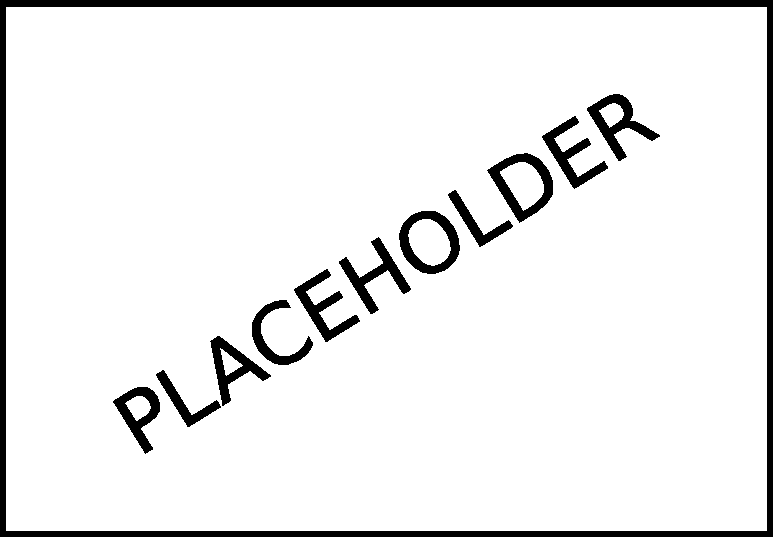
\includegraphics[width=0.8\textwidth]{gfx/placeholder}
    \caption{TODO}\label{fig:cnc-arch}
\end{figure}

\subsection{A basic example}
\label{sec:cnc-basic}
With the paradigm described in Section~\ref{sec:cnc} and the tool provided by AADL presented in Section~\ref{sec:aadl-cnc}, it is possible to define a basic architecture, not only the topology of the connections, but also the internal functioning of the components. As an example, let us take the architecture defined in Figure~\ref{fig:cnc-arch}; in this simple architecture we want to model a robot with two control functionalities: line following and teleoperation.

In the top branch of the architecture we have the line following subsystem: a sensor driver that generates measurements indicating the presence of a black line on the ground and a simple component that directly translate the sensor input in a velocity command. The former expresses a \textit{source} behaviour, it generates messages and circulates them in the system, it is modelled by a process containing a periodic thread, on the frontier there is a output data port. The latter has a \textit{filter} behaviour, it has two ports on its frontier: one input event data port, to queue the messages and trigger a functionality of the component, and one output data port, to send to the next component the velocity commands. In this example, the line following component is very simple and can estimate a set-point directly from the sensor measurements, this means that it does not need to store any information: it is a filter without memory. The internal model of the components is a single thread with an input and an output port, both directly connected to their corresponding ports on the process frontier.

On the bottom branch there is the teleoperation subsystem: a joypad driver providing readings of the input and a teleoperation component to convert the joypad input in set-points. Similarly as the other branch, the driver expresses a \textit{source} behaviour, it converts the input coming from the joypad in messages compatible with the architecture. The teleoperation component, however, does not have the same \textit{filter} behaviour of the line follower, since it stores the incoming messages to smooth the set-point: it is a filter with memory. To model it, it is necessary to define on the frontier of the process two ports: one input event data port and one output data port. Internally, these two ports are connected to two different threads, one is triggered by the event data port, it receive the messages and store them locally. The output data port is connected to a periodic thread, on fixed intervals it reads the two most recent messages and estimate a single set-point compatible with the robot acceleration. Each thread has its own data access to write or read on the shared memory area, modelled as a data component.

In the middle of the architecture, to mediate between the two different control systems, there is a multiplexer component. This is an example of multiple behaviours coexisting in the same component. There are two filters, one for each input, their functionality is to relay the correct message to the output and only one of them is active at a given time, additionally there a \textit{reactive} behaviour. One of the two inputs (\ie, line following or teleoperation) can be selected by triggering a remote function call on the component, which changes a local variable specifying the active input. To model this component it is necessary to define four different features on the frontier: two input event data port, they are the receiving side of the two filters, one output data port, it selectively relays the selected input, and one subprogram access, to trigger the reactive behaviour. Internally, each input port is connected to an independent thread, triggered by the port itself, this threads receive the inputs and store them in a shared memory area. The output port is connected to a periodic thread, which reads the content of the inputs from the shared memory and publish the correct one. The subprogram access interfaces with a thread which has the corresponding subprogram as a subcomponent, this thread is triggered by an external call on the access and changes the current selected input. All the threads have a data access to the same data component representing the shared memory area.

The last element of the architecture is the control component. It is directly connected to the hardware of the robot and consume the set-point provided by the multiplexer to operate the motors, in summary, it expresses a \textit{sink} behaviour. It is modelled by a process containing a single thread, which is connected and activated by the event data port defined on the frontier of the component.

\begin{figure}[t]
    \centering
    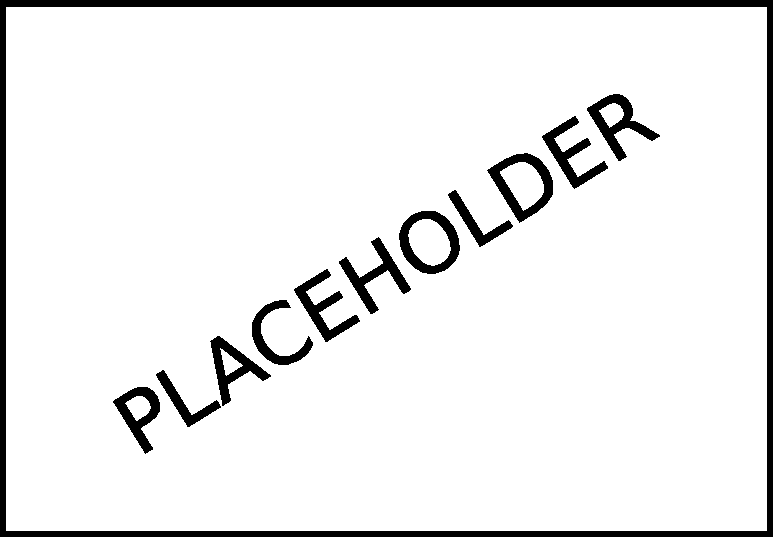
\includegraphics[width=0.8\textwidth]{gfx/placeholder}
    \caption{TODO}\label{fig:connections}
\end{figure}

\section{From C/C to ROS}
\label{sec:cnc-ros}
In Section~\ref{sec:cnc} we already highlighted parallels between the \textit{component-and-connector} paradigm and ROS. At first, it may seem the architectural model of ROS is more complex than a simple component-based approach, since, together with the nodes, there is the extra element of topics, an apparently independent and additional factor. However, topics are nothing more than an agreed name to establish a connection between nodes, they are defined and treated as existing entities in the computational graph, but they do not mediate any communication. After two nodes agree, through mediation of the ROS master, on a communication channel (\ie, a topic), any consequential exchange of messages happens on a direct connection between the two nodes. This means a topics is an aggregation of point-to-point connections and not a independent component mediating the communications. 

Given the actual nature of nodes and topics, it is possible to say that ROS completely follows a \textit{component-and-connector} paradigm, where the nodes are the components and the topics are an aggregation of one or multiple connectors sharing the same characteristics. Figure~\ref{fig:connections} illustrates how all the possible topic configurations (\ie, \textit{1-1}, \textit{n-1}, \textit{1-n} and \textit{n-n}) can be translated in an AADL-based representation, assuming that all the output ports are data ports and all input ports are event data port. The reason of this choice is to model the behaviour of ROS publishers and subscribers. The former does not produce an event notification when it creates a message, it just circulates them in the graph, therefore it is a simple data port, the latter is triggered by the arrival of new messages and supports queue, for this reasons it needs to be modelled as an event data port. As shown in the figure, the substitution process from a topic representation to a connection-based one is quite straightforward. First we select a topic, then we list all the publisher interacting with it, after removing the topic, we directly connect each publisher to all subscribers of the original topic. 

However, by doing this substitution process one piece of fundamental information is lost. In AADL, each connection and each port requires an unique name, this means that it is impossible to maintain the information that a specific connection is part of the aggregation defining the topic. An easy solution is to give the connections a recognisable name, for example each connection for the topic \texttt{/chatter} can have a name starting with \texttt{chatter\_}, however, easy does not translate to good, since this approach is completely unacceptable, it breaks the model by encoding information in variable names. A more elegant solution compatible with the features of AADL is to declare a new \textit{property set}, in this set, called \texttt{topic\_properties}, it is possible to defined two new properties for connections and features. One property is the \textit{Default\_name}, it applies to ports and subprogram accesses, it is used to specify the name of the topic (or service, for subprogram accesses) defined during the implementation of publishers and subscribers. The other property is \textit{Name}, it applies to connections and, at system level, it can be used characterise connections between processes as part of the same topic. The utility of this property is twofold, not only it capture the information of a connection belonging to a topic, but it can be used to include in the model dynamic renaming of topics typical of ROS.

When introducing the concept of component behaviours, we showed how each behaviour can be represented with a specific ROS functionality, however this does not mean that the relationship is bidirectional. ROS imposes very few restriction to the developer, therefore, while the external interface of a node follows the same behaviours presented in Section~\ref{sec:cnc}, the internal implementation may follow an arbitrary pattern. The basic implementation style of a ROS node is to have a main execution loop that periodically polls subscribers and services and pass them the execution every time a new request arrives, similarly to the \textit{component-and-connector} paradigm we presented, this execution happens in a separate environment, however, it is not independent and parallel, but sequential. Practically, this difference it is not meaningful, the conceptual structure presented by the model is the same and this is just an implementation detail. Nevertheless, it is worth to explore an implementation where the actual execution matches completely the description of the model; this will be discussed more in details in Section~TODO. In summary, \textit{sink} and \textit{reactive} behaviours are related to their counterpart in ROS by a bidirectional relationship. It is not possible to say the same when we consider \textit{source} and \textit{filter} behaviours. For reference, let us take the simplest ROS node with publisher functionalities presented in one of the basic ROS tutorial\footnote{http://wiki.ros.org/ROS/Tutorials/WritingPublisherSubscriber(c++)}. In this example, it is possible to see how it is common practice to define a single execution path where everything (\eg, initialisation, polling, publishing, \etc) happens, while this approach is sustainable for small implementations and node with simple behaviours,  it is not suitable for more complex components. This is especially true when implementing components that express multiple \textit{filter} with memory behaviours, in this cases to ensure maintainability, flexibility and understandability of the design it is necessary to follow an approach more in line with the \textit{component-and-connector} paradigm, where each different input and output is managed by an independent execution path. In summary, given the flexibility of the ROS middleware, it is not possible to guarantee that all the implemented node will follow, internally, the design of the \textit{component-and-connector} paradigm. However, the aim of this work is to provide a general modelling approach that can be used to enhance the existing design practices for robotic software, therefore, we will present a way to model (see Section~\ref{sec:ros-in-aadl}) and implement (see Section~TODO) ROS nodes following a simpler, more flexible, easier to maintain and more robust design aligned with the \textit{component-and-connector} paradigm.

While describing the relationship between component behaviours and ROS node implementations, we introduced a key element of any robotic component: the main execution loop. It is in charge of multiple critical tasks of the component; some examples are initialisation, management of incoming requests, dynamic reconfiguration (when supported), error management, shutdown and clean-up procedures. Its role is very important but it is often left out in the modelling phase because of its implicit nature (often hidden by the framework) as the backbone of the component. Nevertheless, it is very important to include it in the modelling process, because some of its tasks may need to be specialised by the developer (\eg, initialisation, error management, \etc). In ROS, in particular, given the freedom left to the developer, it is critical to model the main execution loop to highlight the different functionalities of the nodes, since, as described before, they are often merged in a single execution path. This is another case where for the sake of creating a more general approach and to enhance the ROS design of nodes we, with our modelling approach, overrode the flexibility of ROS to make the main loop an independent execution path disconnected for any other functionality-related path. In summary, in our model, each ROS node, independently from its behaviour, has an additional thread that manages the core functionalities of the component.

\begin{figure}[t]
    \centering
    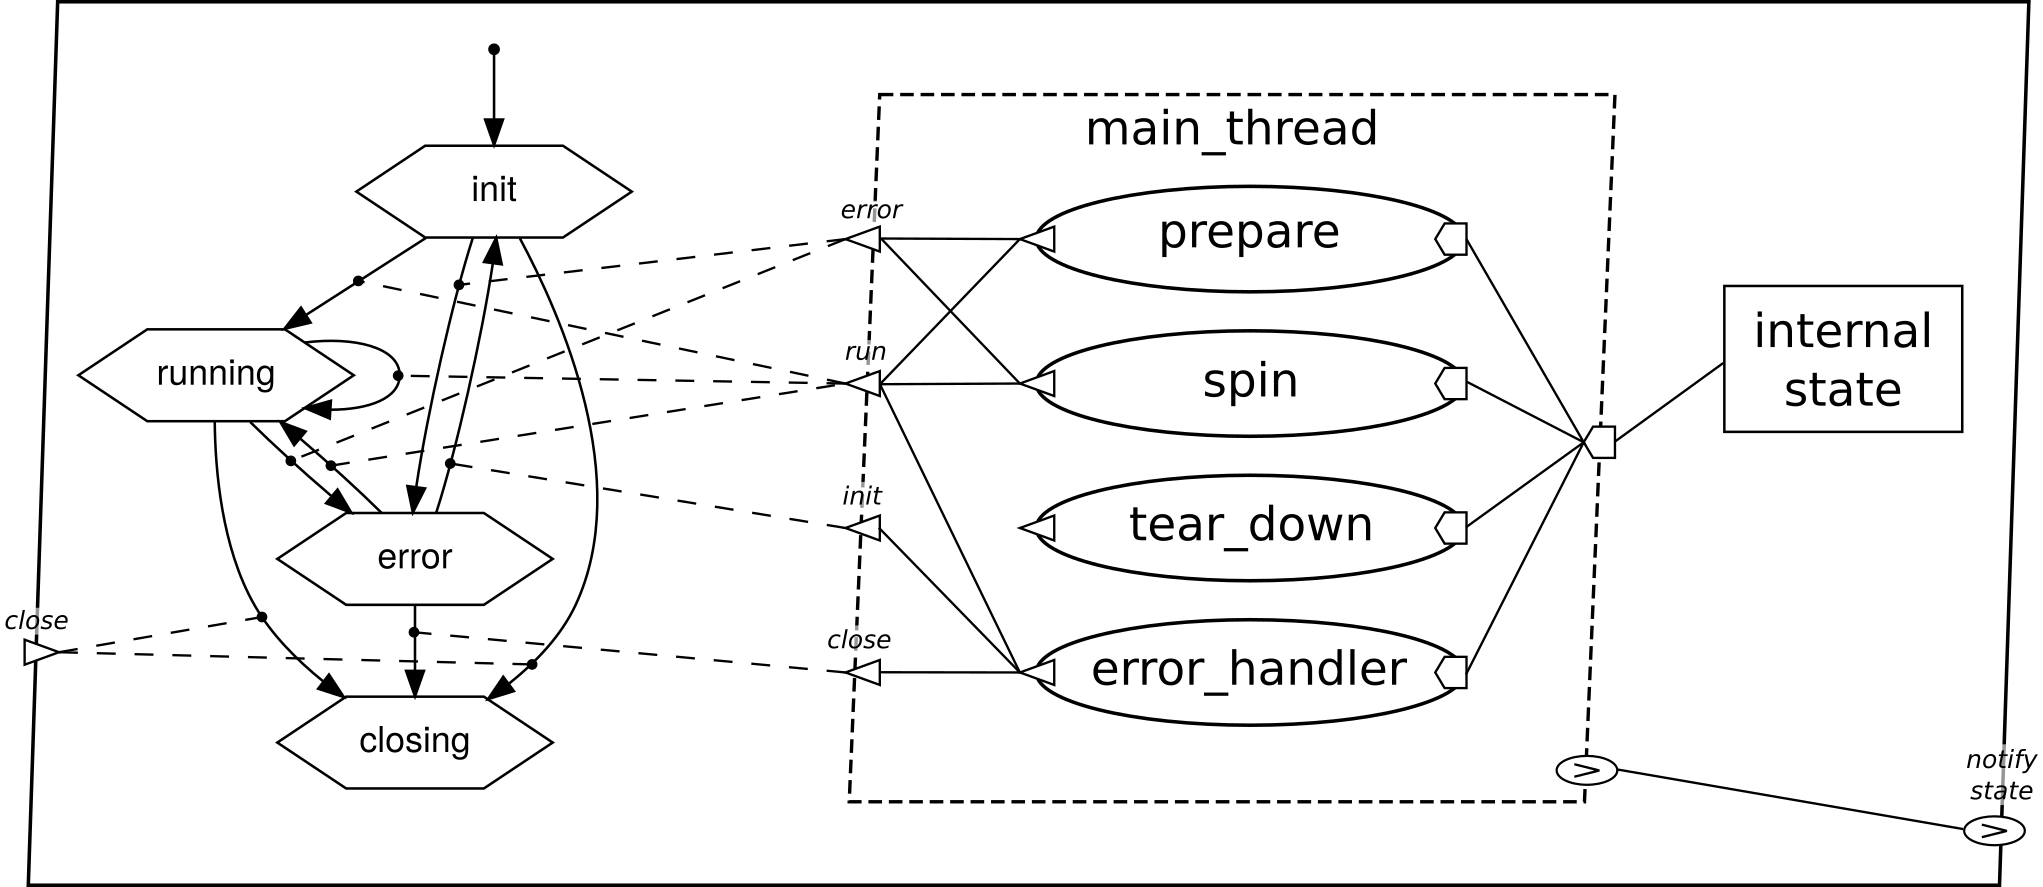
\includegraphics[width=0.95\textwidth]{gfx/essential}
    \caption{TODO}\label{fig:essential}
\end{figure}

\subsection{Modelling a ROS node in AADL}
\label{sec:ros-in-aadl}
In the previous sections, we introduced all the elements we need to model a ROS node: the \textit{component-and-connector} paradigm, how it applies to ROS and the missing elements to bridge from a conceptual model to technological design, and the corresponding AADL description. In this section, we provide a full description of a ROS node, providing first a model of an essential (\ie, no component behaviours) component and then modelling additional functionalities.

Figure~\ref{fig:essential} provides a graphical representation of an essential ROS node. At first glance, it is clear that the model captures more information than what we described until now: the component contain a state machine that is triggered by multiple event ports, the main execution path is detailed by various internal functionalities, there is a permanent internal state and two new features appears on the frontier of the component. Let us analyse the model in order by starting from the state machine: it is used to model the internal life cycle of the component. In ROS there is no defined evolution of the status of a node, usually it can be in only two different states: not executing and active, and the only way to check the current status is to trigger one of the functionalities of the node (\eg, read a topic). However, it is common in component-based approaches to define a clear life cycle of the component, moreover, other robotic middleware and frameworks have an established evolution of the status of their components (\eg, SmartSoft and Orocos), therefore, modelling the internal state machine is a requirement to guarantee the generality of our approach. Our life cycle follows a quite standard structure with four different states.

\paragraph{Init} Initial state of the the life cycle, all the initialisation procedures happen here. After leaving this state it is guarantee the component is ready to execute all its functionalities. From \textit{init}  the component can transition to \textit{running}, when all the initialisation procedure are completed successfully, \textit{error}, or \textit{closing}.
\paragraph{Running} Normal operational state of the component. In this state all the main functionalities are active and the component is working with no issues. The possible transition are: to \textit{running}, the state machine periodically triggers a self loop to ensure that the component is alive and functional, to \textit{error},  or to \textit{closing}.
\paragraph{Error} The component transitions in this state when it captures known errors. While in this state the component is not in execution and recovery procedure can be activate to correct the errors and transition back to an active state (\ie, \textit{init} and \textit{running}), or if the error is unmanageable or catastrophic, to transition to the \textit{closing} state.
\paragraph{Closing} Final state of the life cycle, all the clean up and shut down procedure happens in this state. The transition to this state is triggered by any shutdown signal (internal or external), or when the nodes encounters a catastrophic error that cannot be recovered and requires the node to shut down.
\medskip

Transitions in the state machine are triggered by event ports on the main execution path of the component and on the external frontier. The event port on the frontier is used to model any external signal used to force the shutdown of the node (\eg, SIGINT signal), it triggers the transition to the \textit{closing} state from all active states. All the ports on the main execution thread represents the normal evolution of the system and are activated every time one of the execution phases of the component finishes or when it encounters an error.

The main execution path of the component is modelled using a periodic thread called \textit{main\_thread}. The thread has four subprograms as subcomponents and they represent the active functionalities during each phase of the life cycle. This relationship can be enforced by AADL, since for each state it is possible to specify exactly which subcomponent is active, therefore, while the \textit{main\_thread} is always enabled, only one of its subprograms is active at any given time. Since each subprogram is in charge of a specific state, they are all connected to their corresponding event port to trigger a transition to the next state. Each subprogram has a specific functionality.

\paragraph{Prepare} It is active in the \textit{init} state. This subprogram is in charge of managing node initialisation; it sets parameters, initialise variables, set up publishers and subscribers, and any other node specific initialisation activity. It is connected to the \textit{run} and \textit{error} event ports, to trigger the two possible transitions related with a successful or unsuccessful initialisation.
\paragraph{Spin} It is active in the \textit{running} state, and here the ROS spinner is implemented. When this subprogram is active the \textit{main\_thread} acts as a coordinator of node behaviours, it checks for incoming events and handles potential errors. Two event ports are controlled by this subprograms: \textit{run}, to trigger the self-transition and keep the component active, \textit{error}, to transition to the \textit{error} state when necessary.
\paragraph{Error\_handler} It is active in the \textit{error} state. Here are implemented all the functionalities to deal with known errors of the component, for example an incorrect initialisation or a malformed message. From the \textit{error} state it is possible to transition to any other state, as a result this subprogram is connected to the \textit{run}, \textit{error}, and \textit{init} ports.
\paragraph{Tear\_down} It is active in the \textit{closing} state. This subprogram implements all the procedures related to node shut down. For example, in some cases a node may need to notify another before shutting down, or it need to gracefully disconnect from a physical device. Since this is the final state of the life cycle, this subprogram is connected to no event port on the thread frontier, even so the corresponding port on the subprogram is still modelled for flexibility and potential future extensions.
\medskip

As a final note on the node life cycle, we have included in the model of this essential node a \textit{requires subprogram access} on the frontier of the \textit{main\_thread} which is connected to its counterpart on the process. This access models a remote function call to notify an external supervisor about the current state of the node and any transition. In this way, not only the component has a clear life cycle that defines the execution phases, but it is possible to monitor the evolution of the status through time and keep track of any unexpected behaviour.

Last element to cover is the \textit{internal\_state}, it is a data component used to model the execution memory of the component. In Section~\ref{sec:cnc}, we described how not all the component behaviours requires a shared memory area, therefore, it should not be necessary to include a data component in an essential node. However, in practice, only the simplest component does not require a persistent internal state, because this shared memory area does not exist only as a way for different thread to exchange information. It stores configuration parameters, error mappings, information for shutdown procedures, \etc, for this reasons, not only it is present in this minimal node, but it directly accessible by all subprograms in the \textit{main\_thread}. Since AADL is not a data modelling language (see Chapter~\ref{ch:AADL}), we will not detail here the inner structure of the \textit{internal\_state}, this topic will be covered in Section~\ref{sec:data}.

After modelling an essential node, and by using it as a starting point, we can now add behaviours and functionalities. Figure~\ref{fig:sample-node} shows a graphical representation of a more complex node expressing two coexisting behaviours: a \textit{filter} with memory, modelled with a combination of a \textit{callback} and a \textit{publisher}, and a \textit{filter} with no memory, defined with a subscriber and a publisher in the same thread and identified by the name \textit{callback\_pub}. As introduced in Section~\ref{sec:cnc-ros}, behaviours are modelled using a combination of thread and corresponding ports. In the figure it possible to see how each thread is characterised by a specific port that evokes its functionality: the \textit{callback} has an input event data port, to receive messages and manage queues, the \textit{publisher} has an output data port, to circulate messages to the rest of the architecture, and the \textit{callback\_pub} is a combination of both and has input and output ports. Each port on the thread frontier is then connected to its counterpart on the process to relay from the inside of the component environment to the outside, or vice versa. What is not visible from the figure is the data components associated to each port. In AADL, it is possible to specify the data type exchanged on a connection, and the model will automatically verify that the ports are compatible. Listing~TODO shows a fragment of AADL code where data components associated to ROS messages are declared and used to specify the data type of an hypothetical publisher and subscriber. More details about ROS messages and their definition in the model will be discussed in Section~\ref{sec:data}.

\begin{figure}[t]
    \centering
    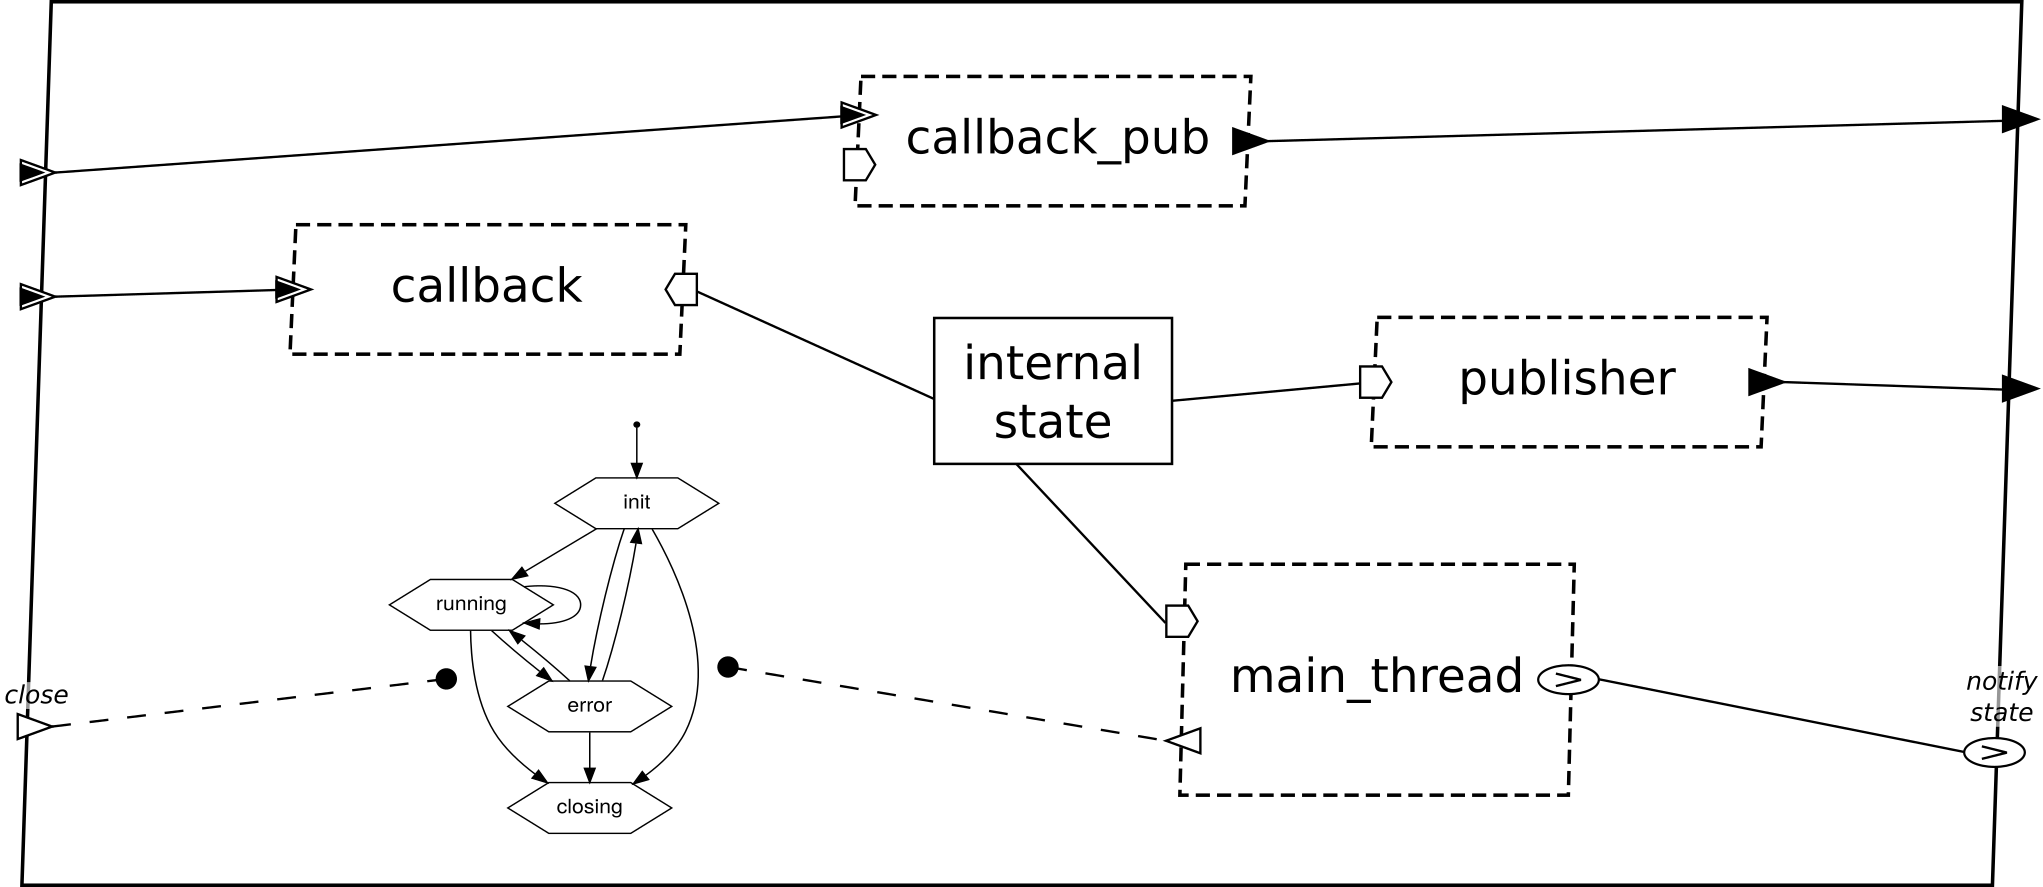
\includegraphics[width=0.95\textwidth]{gfx/sample_node}
    \caption{TODO}\label{fig:sample-node}
\end{figure}

\subsection{Modelling a ROS architecture in AADL}
\label{sec:ros-arch}
In Section~\ref{sec:aadl-robot}, we presented multiple reasons why AADL is a suitable language for robotics, one of them was the capability of the language to model both software and hardware components, however, in our descriptions on how to model ROS nodes we never mentioned any physical interface. The reason for this is that we followed a top down approach to describe a robotic architecture, at higher level of abstraction (\ie, in the \textit{component-and-connector} paradigm) there is no need to make a distinction between a software component and an hardware component, but now that we are moving closer to the actual implementation, this characteristics of AADL will be integrated in our model. We will specify how hardware components can be integrated in the architecture and how to differentiate between communications happening on ROS topic and other physical communication channels. When describing models closer to the implementation level, we also encounter design solutions that are not captured at a more abstract and general level, in ROS there are three key design features that we decided to specifically model in our approach. First of all, existing packages and nodes, the greatest resource of ROS is its repository of already available components, it is imperative to be able to model them correctly in an architecture. Second is \textit{tf}, the coordinates frame manager, it is a backbone of various ROS nodes, therefore it is necessary to include it in the model. Last, it the \textit{actionlib}, an interface to start, monitor, pre-empt and cancel remote tasks, while it is not a commonly used design approach, it is a very useful and elegant way to delegate and coordinate complex task between components.

\paragraph{Physical devices} AADL offers multiple hardware categories to model the physical aspects of a system. For elements like processors or memories we will not go in details, since they work for robotic architectures in the same way of any other, it is possible to bound a software component (\eg, processes or data) to its physical counterpart (\eg, processor and memory) to specify the hardware implementation of the system. In ROS this feature of AADL can be used to model distributed architectures, by binding components to different physical platforms, the designer can specify where each node will be executed at runtime. This creates a deployment view of the system without the need of defining a different model, moreover, AADL analysis capabilities can be used to determine if a specific platform is suitable for a specific subset of the components (\eg, does the target computer has enough RAM to run the system?).

\begin{figure}[t]
    \centering
    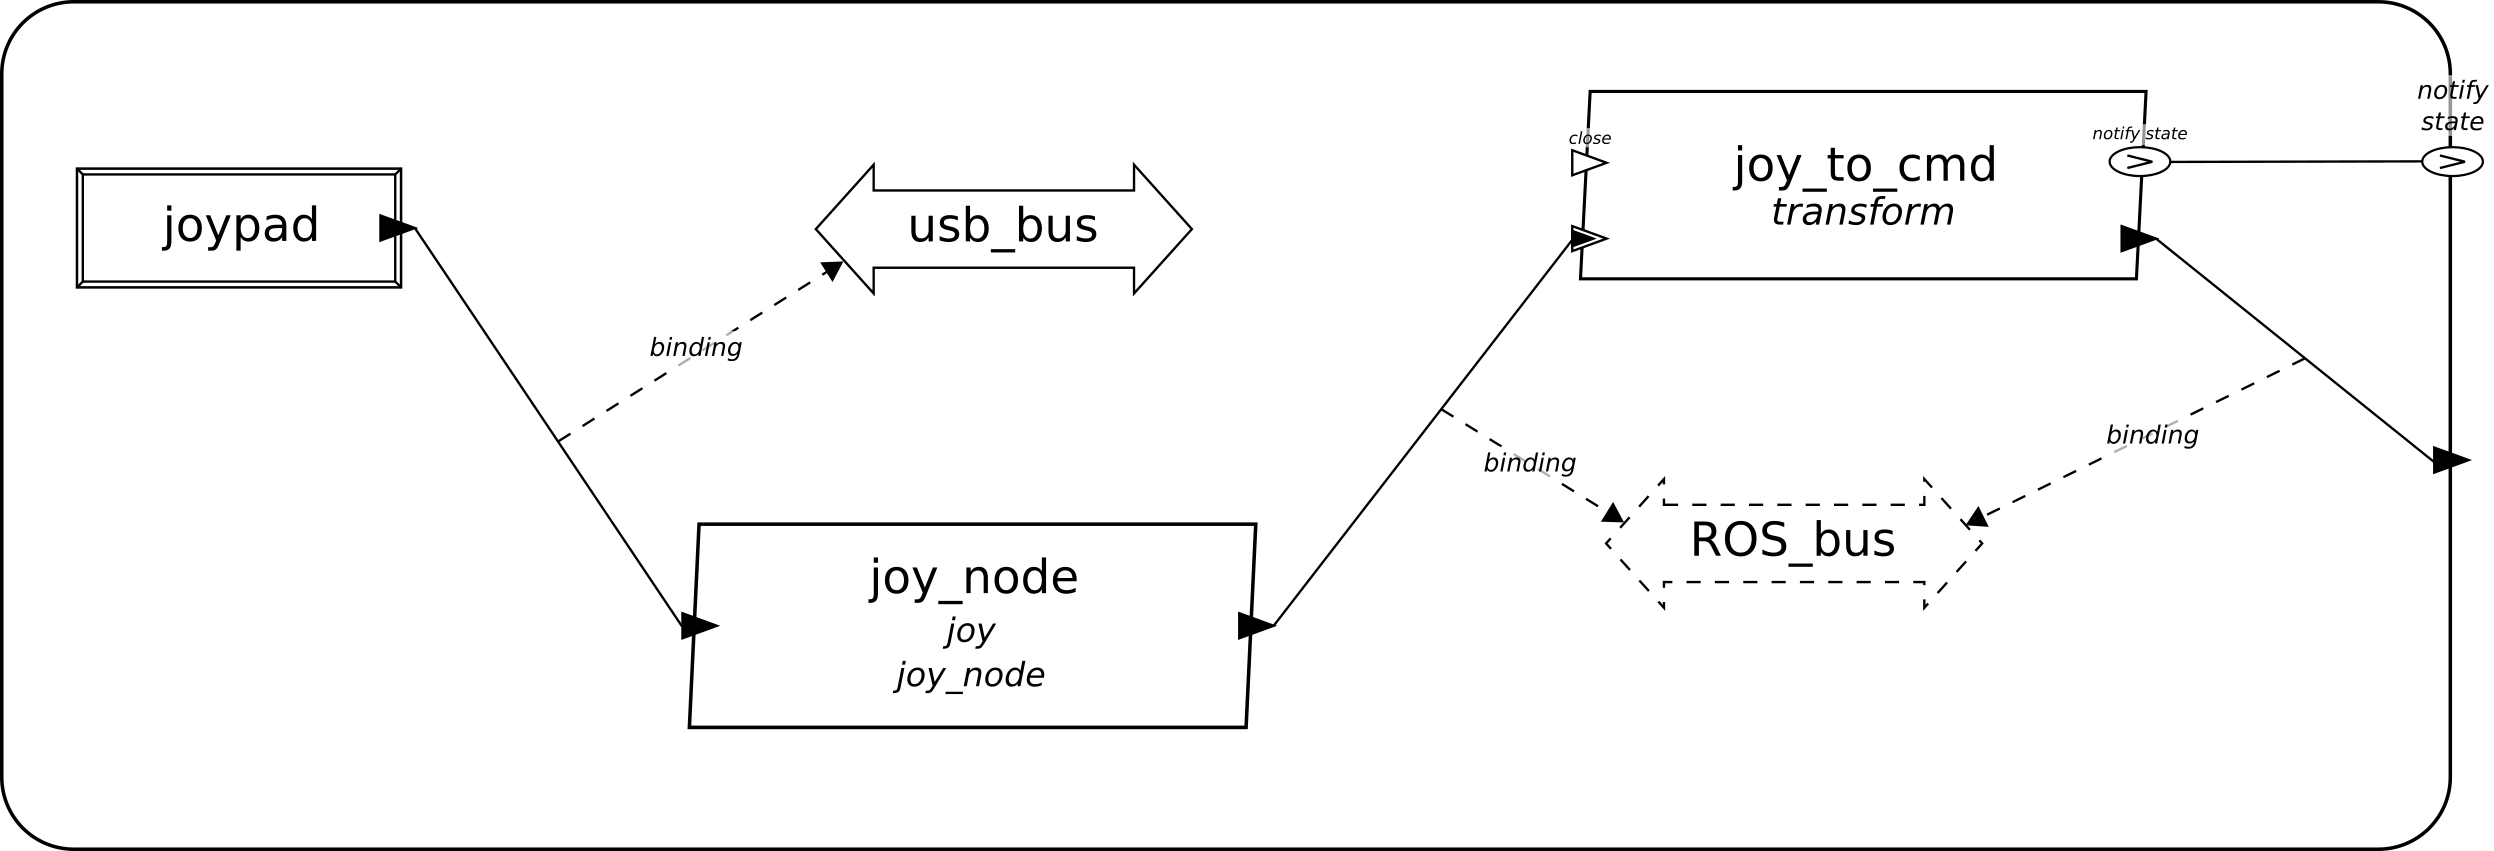
\includegraphics[width=0.95\textwidth]{gfx/mini_arch}
    \caption{TODO}\label{fig:mini-arch}
\end{figure}

What is different in a robotic system is that sensors and actuators are integral part of it, to model them it is possible to use AADL devices. A \textit{device} represents an interface between the physical world and the architecture, it can be modelled as a simple interface or to include the inner functionalities and characteristics of the physical component (\eg, type of communication, computational power, data type).  Devices can connect to processes using ports or accesses, in the same way as processes connect to each other. When modelling a ROS architecture, the fact that physical devices and software components communicate using the same interface rises the issue of differentiate between a topic-based connection and other types of connections; the solution comes in the shape of AADL physical and virtual buses. A \textit{virtual bus} can be used to model abstract communication channels, like ROS topics, while a \textit{bus} can be used for physical connections, like Ethernet and USB. Figure~\ref{fig:mini-arch} shows how this two categories, together with a device, can be used to model a simple joypad-based teleoperation subsystem where a physical bus called \textit{usb\_bus} is bound to the physical connection between the device modelling the joypad and its driver, and a virtual bus called \textit{ROS\_bus} is bound to all the connections representing topics.

\paragraph{Existing ROS nodes} ROS is currently the most popular and widespread robotic middleware, this creates a very prolific and active community, which becomes one of its greatest resources. Given ROS component-based structure and popularity,  a multitude of already existing packages and nodes exist that a developer can simply download and include in his architecture. When creating a modelling approach for ROS it is mandatory to include the possibility to model existing node, to do so we can exploit the dual representation based on component type and implementation provided by AADL.  Existing ROS packages are modelled directly as AADL packages, while existing nodes are modelled using the component type only, basically we provide an interface that appears and behave in the same way as the already existing component, but we do not model in any way the internal functioning. In Figure~\ref{fig:mini-arch}, \textit{joy\_to\_cmd} is a custom made node, completely modelled as visible from the \textit{close} port and the \textit{notify\_state} subprogram access, on the contrary, \textit{joy\_node} is an existing node from the package \textit{joy}, here only topic related ports are modelled to provide an interface to the rest of the system. Listing~TODO shows the textual AADL used to model a ROS packages and node interfaces and how it is then used in an architecture, moreover, it is possible to see how the model descriptions follow the same naming conventions of the original package, while the node name used in the architecture description corresponds to the runtime identifier.

The only potential issue is to create all the models for the existing components, there are few possible solutions that combined can almost automatically generate them. First, analyse the existing nodes at runtime to detect which topics and which messages they use, additionally it is possible to do code inspection to list all the publisher and subscribers, lastly, most packages are documented on the ROS wiki\footnote{http://wiki.ros.org/joy} with, at least, the list and type of topics. Unfortunately, sometimes this is not enough, the joypad driver is one of those example, to detect automatically the connection with the physical device is extremely difficult, at this point the only solution is the human intervention.

\paragraph{tf} This package is one of the core functionalities of ROS and it exists to help manage multiple coordinate frames and transformations over time. Differently from other ROS features, from the point of view of the developer the access to \textit{tf} does not go through any established communication channel (\ie, topics or services), but by using a set of APIs that directly access the distributed coordinate system, additionally, there is no need to start a node to enable it. Therefore, disregarding how \textit{tf} is practically implemented in the system, we can describe it as a centralised resource where all the coordinate frames of the robot and their evolution in time is stored, and it is possible to read or update the content of this shared resource by using specialised APIs. With these assumptions, the best way to model \textit{tf} is to use a single data component at system level that all the nodes can access through data accesses when necessary. The single data component stores the description of the coordinate frames and their evolution in time, while the data accesses represent the bidirectional APIs.

\begin{figure}[t]
    \centering
    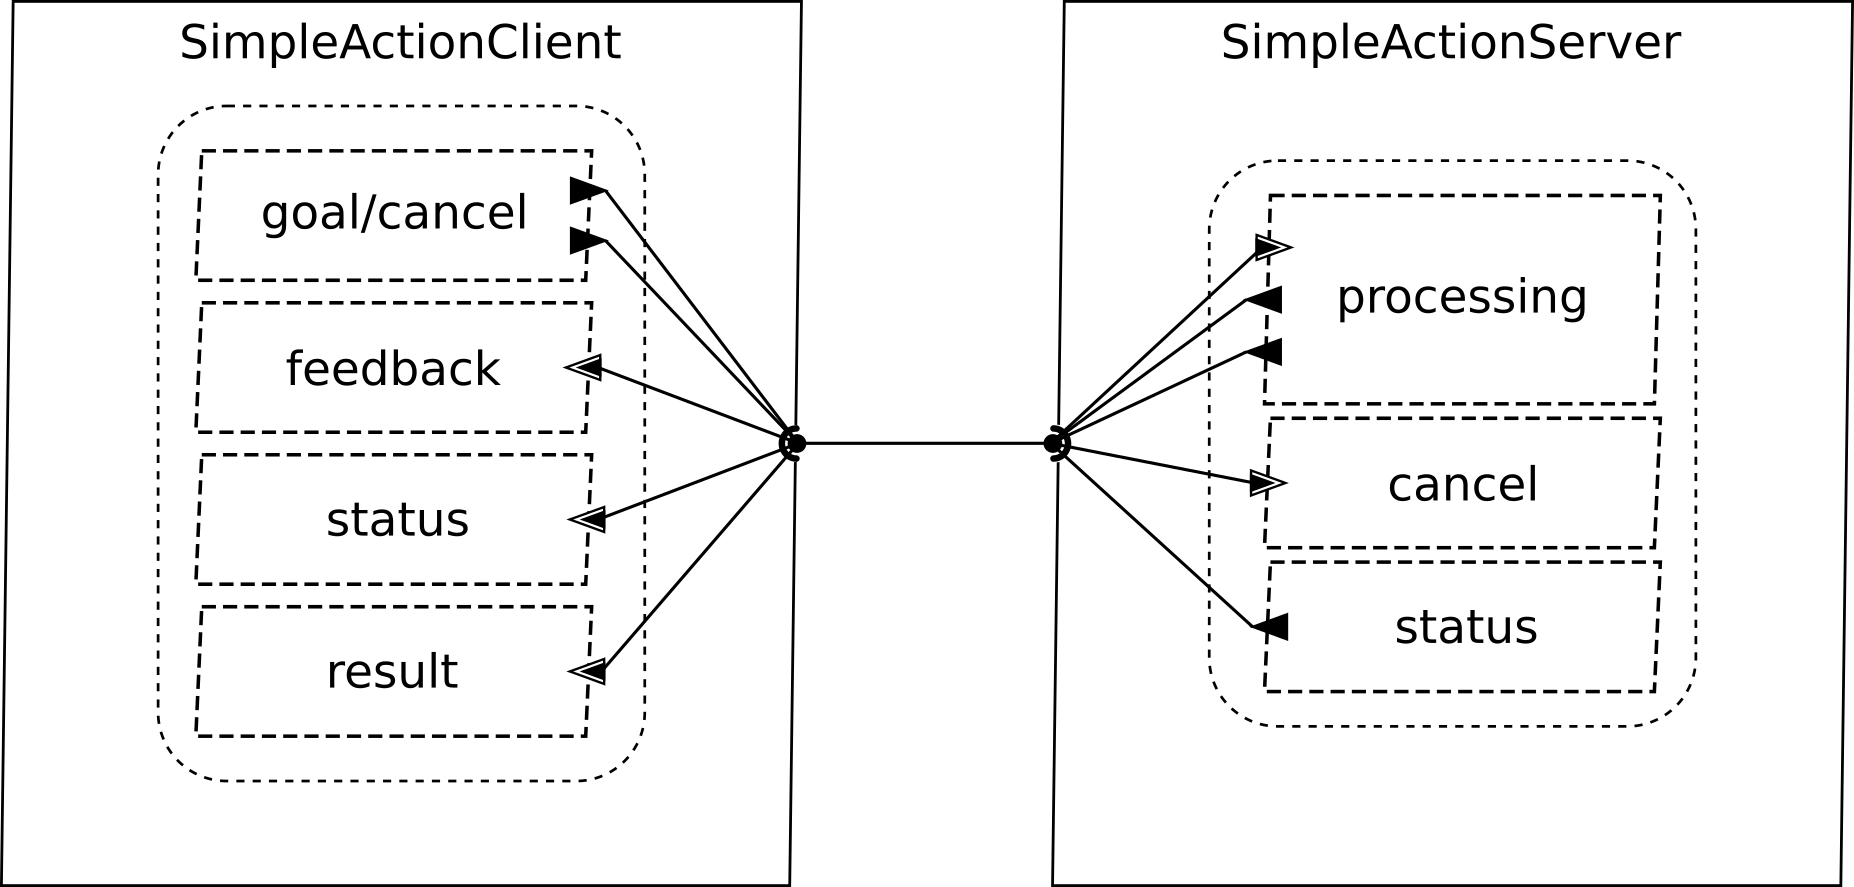
\includegraphics[width=0.95\textwidth]{gfx/action}
    \caption{TODO}\label{fig:action}
\end{figure}

\paragraph{actionlib} Actions are an extension of ROS services, created to manage requests that are too computationally heavy for a traditional client/server approach. An action client can trigger a remote execution on an action server, then resume normal functioning while waiting for a response, if needed. While an action is under execution it sends periodic updates of its status and the original caller can terminate it before it finishes. The actual implementation of ROS actions is based on topics that are used to trigger or cancel the execution, provide the result, and get updates on the status.
% To be able to model correctly an action, it is also necessary to be able to model custom messages, since actions are defined using a \textit{.action} file, which has the same structure of ROS messages, with the difference of being divided in three parts: goal definition, result description and periodic feedback. In our model we use ASN.1 in combination with AADL to do so; the type of the message is defined using a \textit{data} component, in this way AADL syntax will automatically verify the compatibility between the topics, while the actual description of the type it is done using ASN.1, which match the expressive power of the ROS message description language, and, additionally, it provides specification for extra constraints. 
When implementing the action client and server in a ROS node, a developer has to use two already provided classes: \textit{SimpleActionServer} and \textit{SimpleActionClient}. These two classes act as an interface hiding the underlying topic-based system. In AADL it is possible to do the same using a \textit{thread group}; as the name suggest, it is a subcomponent used to group threads together and organize them. Fig.~\ref{fig:action} shows a graphical representation of how an action can be modelled. The client thread group has two outbound ports representing the \textit{goal} topic, used to activate the action, and the \textit{cancel} topic, used to cancel the action; these two ports have their corresponding version on the server group as inbound ports, this time used to trigger the callbacks. The group modelling the \textit{SimpleActionServer} has three outbound ports used to communicate with the client, these ports have their equivalent on the client group. Modelling is about abstracting the underling implementation and representing concepts, therefore at process level the ports of the thread group are aggregated in a \textit{port group}; this maintain the conceptual representation of the action acting as a single communication channel.

\begin{figure}[t]
    \centering
    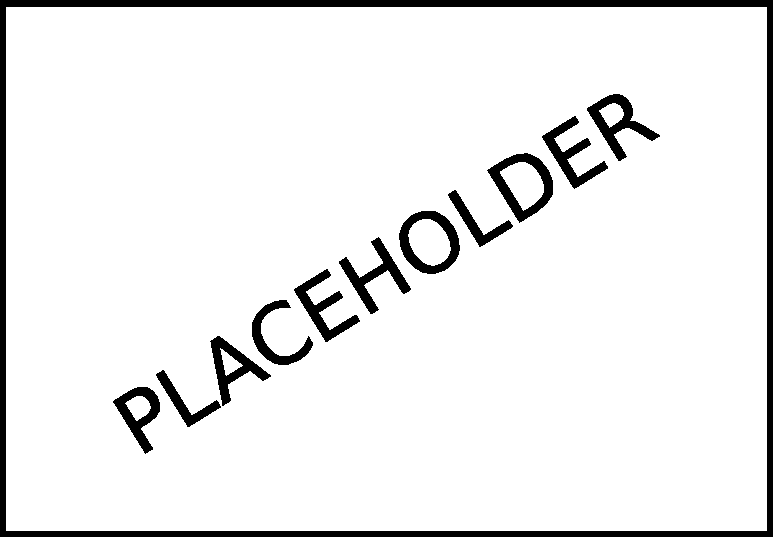
\includegraphics[width=0.8\textwidth]{gfx/placeholder}
    \caption{TODO}\label{fig:ros-arch}
\end{figure}

\subsection{A ROS basic example}
In Section~\ref{sec:cnc-basic}, we presented how to model a simple architecture using AADL and following the \textit{component-and-connector} paradigm. In this section, we describe how that architecture can be updated to represent a complete ROS-based system. As visible for Figure~\ref{fig:ros-arch}, the functionalities of the architecture are the same: line following and teleoperation. However, in this updated version, we include ROS specific elements and we model physical components of the system.

Let us start again from the top branch of the architecture: the line following subsystem. From a pure software point of view, the architecture is unchanged, it consists in two components, one expressing a \textit{source} behaviour and the other a \textit{filter} behaviour with no memory. The difference is in the internal representation of the components, now nodes, which is based on the essential node defined in Section~\ref{sec:ros-in-aadl}; it includes the main execution loop, the internal life cycle and the internal state. Both these nodes are assumed to have application specific functionalities, therefore are fully modelled as custom nodes. From an hardware point of view, this subsystem now includes a physical device: the line detection sensor. It is modelled using an AADL device and it has a physical connection with the driver component. The connection is modelled using an output data port on the device and the corresponding input data port on the process, to specify that it does not represent a ROS topic, it is bound to a physical bus that models an USB connection.

The bottom branch is similar to the example presented in Figure~\ref{fig:mini-arch}. On the software side, the teleoperation component is unchanged, but now it is modelled as a ROS node instead of a generic \textit{filter} with memory component, the driver component is replaced by the already existing \textit{joy\_node}, therefore it is modelled only using the external interface. As for the line following subsystem, now the teleoperation subsystem includes the physical device; it models an USB joypad and it is connected to the driver through a data port. Since this connection is a physical UBS connection, too, it is bound to the same physical bus as the connection between the line detector and its driver.

The multiplexer component is now a ROS node. The original \textit{filter} behaviour is now replaced by a set of two subscribers, they collect the messages coming from the two different subsystems, and one publisher, it relays the correct message to the control component. The \textit{reactive} behaviour is implemented using a ROS service, its functionality is the same, an external client can call this service to change the selected input from line following to teleoperation and vice versa.

The control component is now a control subsystem. In the previous version of the architecture, there was a single component expressing a \textit{sink} behaviour, now, the component is replaced by a custom ROS node with a subscriber to receive the set-points and a device modelling the electrical motor. In this case the interaction between the driver and the motor goes through an Ethernet connection, therefore we modelled a second bus component representing this type of connection.

The architecture includes a virtual bus representing ROS topics, all virtual connections (\ie, topics and services) are bound to this bus. While not visible in the figure, the architecture includes data components for message types. Each type is represented by a data component in same package as defined by the existing ROS hierarchy. The data  type of a port is specified in the process definition and port connected together must have the same data type.

\begin{figure}[t]
    \centering
    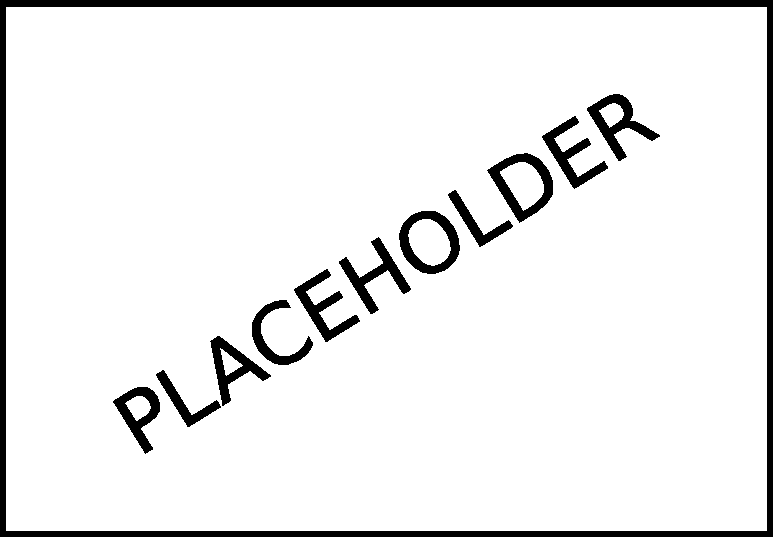
\includegraphics[width=0.8\textwidth]{gfx/placeholder}
    \caption{TODO}\label{fig:template}
\end{figure}

\section{Modelling templates}
\label{sec:template}
With the model definition presented in the previous sections and the ROS-specific models introduced in Section~\ref{sec:ros-arch}, a designer has all the necessary tools to model a functional complete ROS architecture. However, this result does not come without complications, assuming a person is already familiar with AADL, the process of modelling a single architecture is quite tedious and prone to errors, especially replicate the same basic design for all ROS nodes. Moreover, this model aims to be a stepping stone for automatic code generation, for this reason it is necessary the structure of the model is consistent. In summary, there are few issues that need to be addressed:
\begin{enumerate*}[label={\alph*)}]
\item make the modelling approach more accessible, so it can be a reasonable alternative to the current development process for ROS,
\item enforce the presented structure, without it being a burden to the design process,
\item make the underlying structure self-explanatory, without the need of a lengthy accompanied documentation.
\end{enumerate*}

Solving completely all these issue is a very difficult task. In small size project, the process of modelling will always be more complex and time consuming than direct development, until we achieve perfect code generators.  Moreover, there is a limit on how much it is possible to enforce a specific structure, because there is a trade off between the flexibility of an approach and the number of functionality that is possible to model or implement. Nevertheless, in an effort to solve these issues, we developed a series of modelling templates that a designer can use to simplify the modelling process, to do so, we exploited the inheritance capabilities of AADL.

Figure~\ref{fig:template} shows the hierarchy of packages and components when modelling a ROS architecture, and the frontier between the existing templates and the user-created model. At the top of the hierarchy there is the \textit{component-and-connector} paradigm. Here, the main elements of the paradigm are modelled: the component and its implementation, the shared memory area and the inner functionality of behaviours.To model the threads of the behaviours, we used again a hierarchical approach: all behaviour interfaces inherit from the same parent thread which implements the access to the shared memory area as the only common characteristic, then they specify independently their own port to characterise the type of behaviour, only the implementation of the common parent exists since the internal description is always the same (\ie, a single subprogram).

The ROS AADL package extends the \textit{component-and-connector} packages. Here all the necessary elements to model ROS nodes and architectures are defined. The ROS specific elements are modelled directly with no inheritance required, these are: the data component representing \textit{tf}, the virtual bus bound to ROS communications, the main execution loop of the node, and the subprogram associated with the life cycle notification. All the other elements are inherited from the description of the \textit{component-and-connector} package: the node and its implementation extend the component definition, each thread interface extends the corresponding high level behaviour interface (\eg, \textit{service\_provider} extends \textit{reactive}, \textit{callback} extends \textit{sink}, \etc) while the thread implementation extends directly the behaviour implementation. One exception is the ROS timer, since it does not have a corresponding behaviour (it does not interact with the external environment) but it can be used to describe internal functionalities of the node or to give flexibility to the designer, it inherits directly from the general \textit{component\_behaviour} thread. This create the equivalent of a ``ROS node behaviour library''. One element that is necessary to enforce when developing a ROS node is the data type associated with a specific topic, unfortunately the data type of a port is not a mandatory property in AADL. Our solution is to use AADL prototypes; they can be used to create a placeholder for any component or subcomponent. In the thread definition for ROS behaviours, we specified data prototypes associated with the input or output ports, the designer is then forced to specialise them before instantiating the model. Listing~TODO shows how prototypes are defined for the \textit{callback} thread and Listing~TODO shows how they are used in a node definition.

At the lower level of the inheritance there is the specific package to be designed. Other than including the ROS AADL package, it includes all the packages associated with existing ROS nodes and messages. When creating a new node the designer can extend the existing base node provided by the ROS packages, and then add all the necessary functionalities directly from the ROS node behaviour library. This makes the process of modelling a node follow the defined structure, while at the same time, it creates a more compact and easier to design model. Listing~TODO shows how a pair of nodes implementing a publisher and a subscriber can be modelled using this approach.

\section{Data Modelling}
\label{sec:data}
So far, in this chapter, we described in details how it is possible to model component-based architectures together with their interactions, and how to transition from them to fully modelled ROS architectures. However, we only mentioned a crucial part of the description: data; this is mostly because, while AADL provides some tools for data modelling (\eg, data components), it is not a fully fledged data description language. In a robotic system, since they are based on a  \textit{component-and-connector} paradigm, data play a key role to support the communication between components that happens, most of the time, through the exchange of messages or parametrised function calls. This role is so important, that most of the robotic frameworks and middleware develop their own language to describe data supporting communications, for example, ROS uses a simple message definition language to put the focus on the creation of custom messages when needed, the same happens for SmartSoft where the communication object are defined using a fully fledged Xtext-based DSL. There approaches exist so the designer of the middleware or framework can have full control on the shape and style of the message definition to correctly implement the low-level communication between components, however, this fragmentation makes the definition of a general purpose data modelling language quite challenging. Since AADL supports data components but it lacks tools for data description, the simplest solution would be to use data component as type identifier and adopt the target message description language as type descriptor. Considering that data components are already software specific, this solution could work for everything related to communication, but it has two important limitations. First, while it works well for already existing messages that can be simply imported in the model, it removes any possibility of generality in the newly defined messages; an ideal solution would use a general description for custom messages that can be associated with different data type depending on the target platform. Second, communication-related data type are not the only type of data present in a system, a general data definition languages could be used to model all data in the architectures.

Beside of communications, there is another situation where data definitions play a key role: parametrisation of the component. When implementing a component there is a series of values that are calibrated for a specific configuration of the robot (\eg, maximum acceleration, camera resolution, wheel diameter, \etc), additionally, some of these parameters may need to change at runtime, both for on-line calibration (\eg, measurement weight during sensor fusion, obstacle avoidance threshold, \etc) and for dynamic functionality change (\eg, indoor vs outdoor operation, high vs low performance, \etc). In practice, different technological solution are used to implement parametrisation. ROS relies on a centralised component where all node parameters are stored and categorised using node-specific namespaces, at any time during execution a node can query the parameter server and retrieve a copy of the value. There is no strict differentiation between initialisation and runtime parameters, although ROS provides a separate system\footnote{http://wiki.ros.org/dynamic\_reconfigure} to perform dynamic reconfiguration. Values in the parameters server are set or via command line before running the node or by loading a YAML file. SmartSoft uses a more complex structure for parameters, there are configuration parameters that are set at deployment time and cannot be changed after the component initialisation, and there are runtime parameters that can be used to configure the component at runtime. Definition of parameters is divided in two categories, too, they can be internal, therefore defined together with and specifically for the component, and external, thus defined as separate parameter sets that can be reused in multiple component. The description itself of the structure of the data is done using a DLS similar to the message definition DLS. In this case there is no simple cohesive approach that can be used to easily import the existing definitions, because parameters, as a concept, are less standardised than communication protocols.

There is one last use of data in a component that is interesting to analyse under the lens of a data modelling approach: internal variables. Components are, in the end, computer programs, thus they may have tens of variables storing any type of value necessary for a successful execution. Of course it is pointless to try to model beforehand all the variables involved in the execution of a component, however, as we described in Section~\ref{sec:cnc}, there is a specific component behaviour, the \textit{filter} with memory, where the type of information stored in the shared memory is defined ad design time, because it is part of the description of the functionalities of the component. For example, let us take a component in charge of obstacle avoidance, the designer knows in advance that the component will store the map of the environment, or a multiplexer component needs to store locally the inputs before relaying them. This design approach is similar to the object-oriented programming paradigm where before starting the implementation the developer design the class with all the necessary attributes and methods. By describing ports and components behaviours, we already defined the component-equivalent of methods, thus it is but a short step to fully embrace this consolidated design approach by defining the component-equivalent of attributes, too. Currently, no middleware or framework, not even those leaning more towards a model-driven development approach (\ie, SmartSoft and Orocos/RoCK) support the definition, at design time, of internal variables of the component. The reason of this lack of support with respect of parameters lies in the difference of complexity between the two; usually parameters are basic types (\eg, string, integer, boolean, \etc) or basic data structures (\eg, record, array, list, \etc), while internal variables can be any kind of object or data structure coming from internal or external libraries, moreover, often they require special initialisations. Unfortunately, given this complexity, we found no reasonable way to preserve the semantic of the internal variables in the same way as we could do for parameters. Nevertheless, we designed a compromise that maintains the semantic for simpler variables (\ie, basic types), but, at the same time, it allows for more complex types to be defined at design time.

These are all the situations in which data modelling is integral part of the design of a robotic application: communication objects, parameters, and internal variables. In the reminder of this section we will cover the two options we explored to be able to model all these features, their specific advantages and their limitations.

\begin{lstlisting}[float,frame=tb,caption={ROS message, service and action definition using ASN.1},label=lst:asn1-ros]
CustomPackage DEFINITIONS AUTOMATIC TAGS ::= BEGIN
	IMPORTS Pose FROM Geometry_msgs;
	CustomMessage ::= SEQUENCE {
		x	INTEGER(1 .. 10),
		y	REAL,
		pose	Pose
	}
	CustomService ::= SEQUENCE {
		request SEQUENCE {
			a  INTEGER(-10 .. 200),
			b  SEQUENCE (SIZE (1..10)) OF INTEGER
		},
		response SEQUENCE { sum INTEGER }
	}
	CustomAction ::= SEQUENCE {
		goal SEQUENCE { },
		result SEQUENCE { },
		feedback SEQUENCE { }
	}
END
\end{lstlisting}

\subsection{Option 1: ASN.1}
Abstract Syntax Notation One (ASN.1) is an interface description language, it is a broadly used standard in telecommunication and computer networking. The language put a lot of focus on encoding and decoding and it is designed to be completely independent from any computer or programming language. For these reasons, we considered it as our first option when trying to model the data exchanged in a robotic architecture.

In ASN.1 a communication protocol is defined in a module, inside, each element of the protocol (\eg, requests, responses, errors, \etc) is defined using a type. Normally, types are instantiated by a protocol data unit (PDU), however, when describing communication patterns, we use only defines modules (\ie, protocol descriptions) since the actual low-level communication is then left to the communication layer of the target middleware or framework. Nevertheless, this general description based on ASN.1, could be used to create a corresponding PDU and, eventually, an inter-protocol communication between different platforms. Listing~\ref{lst:asn1-ros} shows an example on how to model a ROS package containing all the possible user-defined communication objects, in particular a message, a service and an action. In this description, an ASN.1 module correspond to a ROS packages, this binding exists for multiple reasons: first, when importing an existing definition (Pose in Listing~\ref{lst:asn1-ros}), the finest granularity available is the type defined in a specific module, this mirror the behaviour of messages defined in packages, second, modules are the only aggregator of ASN.1, therefore they have the same conceptual functionality of packages, lastly, types are the definition referenced by PDU, in the same way as message instances reference to a message definition in a package.

Messages are the most straightforward to define, since they do not have any internal structure other than the message itself. The are defined directly using a ANS.1 type and the fields uses the same basic types expected in a normal ROS messages, value ranges (\eg, \texttt{INTEGER(1 .. 10)} and \texttt{INTEGER(-10 .. 200)}) can be used to automatically identify the correct size of the target type (\eg, \texttt{uint8} and \texttt{int16}). Arrays can be defined using the keyword \texttt{SEQUENCE OF}, eventually specifying a minimum and maximum size. One of the characteristics of ROS messages is their hierarchical definition, they can always include other messages defined in the workspace, one typical example is the header used to timestamp messages. This is possible in ANS.1 using the \texttt{IMPORTS} keyword at the beginning of the module definition, and then declare a field of a type to be of the imported definition. Of course this raises the problem of creating all the ANS.1 definitions for ROS messages, however, given the simplicity of the message definition language used in ROS, it is a task that can be easily automated to generate all the necessary files for the entire workspace. Internally, service definition is identical to message definition, the same rules are used to define basic types, arrays an to include existing types. The difference is in the structure of the ANS.1 type, for service it is necessary to differentiate between \textit{request} and \textit{response}, in the former, the developer describes the content of the request message sent by the client to the server, the latter contains the expected answer. The description of actions is similar, in this case the type is divided in three subsections: \textit{goal}, \textit{result}, and \textit{feedback}. Each subsection can have an arbitrary number of field defined as basic types or existing types from other packages. For both services and actions, it is possible, in ROS, to send empty messages, for example a service used to trigger a functionality has an empty request, but the result of the functionality as a response. Empty sequences are supported by ASN.1, therefore, the correct way to model a service or an action with empty interactions is to define the subsection but leave it empty, as seen in Listing~\ref{lst:asn1-ros} for the feedback of the action.

\begin{lstlisting}[float,frame=tb,caption={Internal state of a node modelled using ASN.1},label=lst:asn1-ros-is]
InternalState DEFINITIONS AUTOMATIC TAGS ::= BEGIN
	Complex ::= SEQUENCE {
		type	UTF8String,
		include	UTF8String
	}
	Parameters ::= SEQUENCE {
		size	INTEGER DEFAULT 1,
		dimensions	SEQUENCE {
			height	REAL DEFAULT 1.0,
			width	REAL DEFAULT 2.0
		}
	}
	Variables ::= SEQUENCE {
		counter	INTEGER,
		map	Complex
	}
END
\end{lstlisting}

\begin{lstlisting}[float,frame=tb,caption={TODO},label=lst:asn1-ros-is1]
params Parameters ::= {
	size 2, 
	dimensions { height 2.0, width 3.0 }
}

value Variables ::= { 
	counter 0,
	map {type "test", include "test"}
}
\end{lstlisting}

To model the internal state of the node we have to follow a different approach. In this case, it is necessary to define both the module (\ie, the structure of the internal state) and the PDU (\ie, the specific configuration of the internal state), however these two specifications will be used at different times in the design, development and deployment cycle of the architecture. As for the communication objects, everything resides in the same ASN.1 module, but in this case, each module represent a specific node, although, if two nodes share the same parameters and variables configuration, they can share the same module (\eg, different implementation of the same functionality). Listing~\ref{lst:asn1-ros-is} shows how an hypothetical internal state of a node could be modelled using ASN.1, while Listing~\ref{lst:asn1-ros-is1} represent a possible instance. The list of parameters and variables are defined each in their own type. For parameters, the description is quite simple, since they only use basic types and, potentially, nested records. Basic types are matched directly with their ASN.1 counterparts, again the range can be used to automatically specialise type during implementation or to define boundaries for the parameters. Often, parameters related to the same functionality (\eg, configuration values of a planner) are grouped together in a record data structure (\eg, C struct), to achieve the same result it is possible to declare the parameters as nested \texttt{SEQUENCE}. For most of variable definitions the process is the same as parameters, it is possible to use basic types and nested data structure to define and organise basic variables. The difference between the two lays in what we call ``complex'' variables, here the developer is not forced to use only basic types, but can use data structure of unpredictable complexity (\eg, ROS messages for storage, maps, point clouds, behavioural trees, \etc). It is unreasonable to try to capture this complexity in an high level design specification, therefore we defined an extra ASN.1 type called \texttt{Complex}. This type has two fields: \texttt{type}, the actual type of the variable in the target programming language (\eg, \texttt{costmap\_2d::Costmap2D} for a ROS costmap in C++), and \texttt{include}, the resource to be included to use the specific data type (\eg, \texttt{costmap\_2d.h}). The example and the structure presented here is specifically targeted for a C++ implementation of a ROS node, but the concept of the complex variable, can be easily translated to different programming languages. From a design point of view, the variable act as a conceptual placeholder for a more complex implementation, while during code generation the complex description can be used to automatically create the internal state of the component. For the description of the internal state, we can combine the module with the PDU to create a complete definition of the node. While in the module we can define default values for both parameters and variables, their actual values are going to change significantly depending on the particular deployment. To capture this, we can use the PDU to specify the current instance of the internal state, and automatically generate a specific initialisation for parameters and variables; complex variables, of course, are the exception, since the information contained in the PDU are used to define them during code generation.

\begin{lstlisting}[float,frame=tb,caption={ROS message definition using JSON schema},label=lst:json-ros-msg]
{
  "$id": "custom_package/CustomMessage.schema.json",
  "type": "object",
  "properties": {
    "x": { "type": "integer",
      "minimum": 1, "maximum": 10 },
    "y": { "type": "number" },
    "pose": { "$ref": "geometry_msgs/Pose.schema.json" }
  }
}
\end{lstlisting}

\begin{lstlisting}[float,frame=tb,caption={ROS service definition using JSON schema},label=lst:json-ros-srv]
{
  "$id": "custom_package/CustomService.schema.json",
  "type": "object",
  "properties": {
    "request": {
      "type": "object",
      "properties": {
        "a": { "type": "integer",
          "minimum": 1, "maximum": 10 },
        "b": { "type": "array",
          "minItems": 1, "maxItems": 10,
          "items": { "type": "number" } }
      }
    },
    "response": {
      "type": "object",
      "properties": { "sum": { "type": "integer" } }
    }
  }
}
\end{lstlisting}

\begin{lstlisting}[float,frame=tb,caption={ROS action definition using JSON schema},label=lst:json-ros-act]
{
  "$id": "custom_package/CustomAction.schema.json",
  "type": "object",
  "properties": {
    "goal": { },
    "result": { },
    "feedback": { }
  }
}
\end{lstlisting}
 
\subsection{Option 2: JSON with schema}
 JavaScript Object Notation (JSON) is an open-standard file format, it is human readable text where objects are codified in attribute-value pairs and array data types. While it was originally derived for JavaScript, hence the name, it is a language-independent data format, it is very common and massively used for asynchronous browser-server communication. While JSON is excellent to describe object instances (\ie, the actual data content), it is normally used with the assumption that the data structure is codified somewhere else (\eg, in the source code defining the object). However, there are various initiatives to define the structure and the content of the data using JSON, the one we are using in our approach is called JSON Schema; it is a vocabulary to annotate and validate JSON documents. The capability offered by the schema definition, combined with the extreme popularity of JSON made it our second option for data modelling.
 
A complete description based on JSON schema is composed by the schema, created following the vocabulary, and an instance of the data. Following a similar approach to ASN.1, for the description of messages, services and actions, we are going to define only the schema, and leave the instance to the underlying communication protocol. As before, the general description defined using JSON schema, can be used to create JSON documents with the same semantic value of the messages exchanges by the underlying middleware or framework, this is extremely useful since JSON is one of the most common standard for the web, therefore, through this description, it is possible to create a web-compatible interface for the robot. Differently from ASN.1, each schema is not a complete package, but a single message, service or action definition, the same as it happens in ROS. To model the concept of packages it is possible to follow various routes, for example, locate the schema in the same folder, in the same way as ROS does, or exploit the unique id (\texttt{\$id}) to categorise the schema, in our approach we use both. Listing~\ref{lst:json-ros-msg}, \ref{lst:json-ros-srv} and \ref{lst:json-ros-act} show three different schemas representing a message, a service and an action, all of them defined in the same ROS package; physically, these three description are defined in three separate files and are stored in the same folder, exactly as it would happen for ROS definitions in the same package, moreover the \texttt{\$id} is structured to specify both the package and the name of the definition.

As before, messages are the simplest to model, since they do not have any nested structure, and if they do, it is based on a different type. With JSON schema it is possible to directly define the list of field of the message and specify their type. The available basic types are: \texttt{string}, for a string of character of a specified length eventually matching a pattern, \texttt{number}, any type of real number where it is possible to specify the boundaries, \texttt{integer}, a subset of integer numbers, \texttt{boolean}, for a filed that can either be true or false, and \texttt{null}, for empty fields. Additionally a field can be of type \texttt{array} when it represent an array, in JSON there is no restriction on the type of the elements of an array, therefore JSON schema supports multiple options ranging from all the elements having the same type to each element has a different type. In ROS, only same-type array are admitted, in Listing~\ref{lst:json-ros-srv} we modelled an example of a 10-elements integer array. JSON schema supports referencing external schemas, this can be used to model how in ROS message field can be of the type of a previously defined message. Additionally, most JSON schema validators support the use of URL as \texttt{\$id} and \texttt{\$ref}, this means it is possible to use the online location of a schema definition as the id and then use the same location during validation. In summary, only the custom message schema has to be parsed directly, everything else can be remotely checked only when necessary. As always, this raise the problem of generating the schema of all the existing messages, but not only this can be done automatically, they can be collected in a single online library (\eg, ROSWiki) or hosted in the same repository together with the ROS source code. Regarding the description of types, services are defined in the same way as messages. They can use basic types, arrays or reference existing messages. However, their schema is divided in two section defined as two different objects: \textit{request} and \textit{response}. As before, the former describe the message sent to the server to trigger the service and the latter models the answer received by the client. The same structure based on sub-objects is followed by the action description, this time divided in three different parts: \textit{goal}, \textit{result} and \textit{feedback}. Each subsection follows the same rules of the message, can have multiple field as basic types, arrays or reference existing definitions. One significant difference between JSON schema and ASN.1 is how they describe empty messages. In JSON schema empty brackets (\ie, \textit{\{ \}}) represent the wildcard (\ie, it matches every sequence), the correct way to specify an existing, yet empty, field is to declare it as type \texttt{null}, as seen in Listing~\ref{lst:json-ros-act} for the feedback of the action.

\begin{lstlisting}[float,frame=tb,caption={Base schema of the internal state defined using JSON schema},label=lst:json-is-base]
{
  "$ref": "#/InternalStateBase",
  "InternalState": {
    "additionalProperties": false,
    "type": "object",
    "properties": {
      "Parameters": {
        "type": "object",
        "additionalProperties": true
      },
      "Variables": {
        "type": "object",
        "additionalProperties": true
      }
    }
  }
}
\end{lstlisting}

\begin{lstlisting}[float,frame=tb,caption={Internal state defined using JSON schema},label=lst:json-is]
{
  "$ref": "#/CustomInternalState",
  "InternalState": { "type": "object",
    "properties": {
      "Parameters": { "type": "object",
        "properties": {
          "dimensions": { "type": "object",
            "properties": {
              "height": { "type": "number", "default": 1.0 },
              "width": { "type": "number", "default": 2.0 }
            }
          },
          "size": { "type": "integer", "default": 1 }
        }
      },
      "Variables": { "type": "object",
        "properties": {
          "counter": { "type": "integer" },
          "map": { "$ref": "#/complex" }
        }
      }
    }
  },
  "complex": { "type": "object",
    "additionalProperties": false,
    "properties": {
      "type": { "type": "string" },
      "include": { "type": "string" }
    }
  }
}
\end{lstlisting}

\begin{lstlisting}[float,frame=tb,caption={Internal state instance defined in JSON},label=lst:json-inst]
{
  "Parameters": {
    "dimensions": { "height": 2.0, "width": 3.0 },
    "size": 2
  },
  "Variables": {
    "counter": 0,
    "map": { "type": "test", "include": "test" }
  }
}
\end{lstlisting}

As mentioned before, when describing the internal state we have to use both the instance, representing the actual values of the parameters and variables, and the schema, the model that validates the structure of the instance to ensure its compatibility with the component. When using JSON schema we opted for a hierarchical approach based on a double validation. First, we validate the instance to verify the general structure, and then we use the component-specific schema to validate the content. Listing~\ref{lst:json-is-base} shows the schema used for the first step of the validation. The designer has to follow this model, but he does not have to implement or provide it, since it is embedded in the validation and code generation process. The base schema is used to verify that the instance follows the structure where the internal state is divided in two, and no more (see \texttt{additionalProperties} set to false), subsections: parameters, values that are initialised at the beginning of the life cycle of the node and are not subject to changes, and variables, values used to capture the evolution of the internal state of the component. Listing~\ref{lst:json-is} represent the schema of an hypothetical internal state of a component, and it is the definition used in the second step of the validation process. Following the structure enforced by the base schema, parameters and variables are defined each in their own object. Since parameters are defined using basic types and nested records, their description is quite straightforward. JSON schema types are used to define their implementation-specific counterparts, while the \texttt{object} type can be used to define nested records. For variables definition, the process is mostly the same, basic types variables are defined directly using JSON schema types, and it is possible to create nested structures to organise them. Similarly to ASN.1, we defined an new object to capture ``complex'' variables. This object has exactly (enforced by setting \texttt{additionalProperties} to false) two values: type, defines the actual complex type of the variable, and include, in a C/C++ specific implementation it provides the resource to be included to correctly use the complex type. The \textit{complex} object can be redefined to match the requirements of different programming languages, for example, Python does not require a type but may need to specify which resource to import. The schema presented in Listing~\ref{lst:json-is} represents only half of the necessary description to completely model the internal state of a node; it is the static design and it is completed by the JSON instance. An example of an instance compatible with the two schemas presented is in Listing~\ref{lst:json-inst}. 

\subsection{Comparison}
Both ASN.1 and JSON schema are powerful enough to completely capture the description of communication objects and the internal state of the components, therefore they are almost interchangeable as data description language. Additionally, ASN.1 supports JSON encoding rules (JER), so, in theory, it would be possible to create a direct conversion between the two different representations. All considered, it may not be necessary to pick a specific option to model the data in the architecture, however, there are some reasons that make one approach more suitable than the other. ASN.1 is a widely used protocol description language that supports multiple encodings and can deal automatically with various low-level communication issues (\eg, endianness, payload size, \etc), this is extremely useful when modelling communication with physical devices, therefore it can be used when dealing with sensors and actuators. However, ANS.1 can be too low-level for most applications and while widely used it is not a widely known language. JSON, on the contrary, was created to encode JavaScript objects, thus it does not capture low-level details, but it is a de facto standard for web communications and NoSQL databases. This means it can be used to create communication bridges between different technologies (\eg, ROS and SmartSoft), web APIs for robots or advanced logging systems.

In summary, both approaches are suitable for modelling all the data exchanged in robotic systems, but the specific characteristics of the languages make them more or less useful when facing specific problems. 
%*****************************************

%************************************************
\chapter{Automatic programming}\label{ch:code-gen}
%************************************************

\begin{flushright}{\slshape Writing machine code involved several tedious steps—breaking down a process into discrete instructions, assigning specific memory locations to all the commands, and managing the I/O buffers. [...] We needed to understand how we might reuse tested code and have the machine help in programming. [...] This led to the development of interpreters, assemblers, compilers, and generators—programs designed to operate on or produce other programs, that is, automatic programming.} \\ \medskip
    --- Mildred ``Milly'' Kross
\end{flushright}

Creating a computer program is a challenging and engaging experience, it requires expertise, brilliance and ingenuity. At the same time, writing code is a mundane and dull activity, it requires to complete repetitive tasks, to manage multiple small issues and to deal with problems unrelated with the main project.

Thankfully, today, we are not dealing with the same difficulties that Mildred Kross faced when working on the UNIVAC I. Multiple technological advancements and progresses in Computer Science gave us compilers, high-level programming languages, design paradigms, frameworks, middleware, integrated development environments, and more. All these tools exist to make computer programming more about designing and developing a program than writing code. 

During Computer Science history, the concept of automatic programming changed to adapt to the expectation of the time. Originally, it was the automation of the process of punching paper tape, later it became the transformation of high-level programming languages (\eg, Fortran and ALGOL) to machine code, a task that, nowadays, is integral part of the build process. Today, automatic programming mostly refers to the automatic generation of executable code from representations that are not programming languages. These representation may have different level of abstraction, from the closest to the target (\eg, domain specific languages, flowcharts, \etc) to the furthest (\eg, graphical representations, models, \etc).

%TODO complete after the end of the chapter
This chapter presents our approach to automatically generate ROS code from the AADL model.

\minitoc
\newpage

\begin{figure}[t]
    \centering
    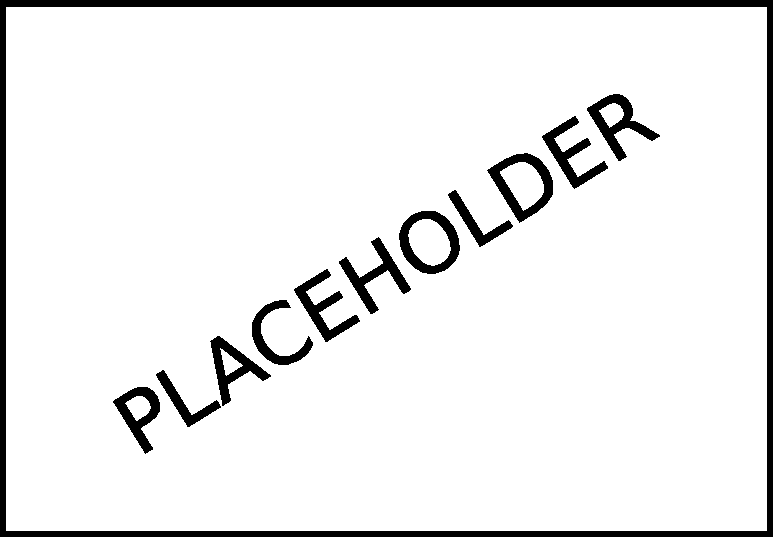
\includegraphics[width=0.8\textwidth]{gfx/placeholder}
    \caption{TODO}\label{fig:code-gen}
\end{figure}

\section{Generating ROS artefacts}
An automatic programming approach is a collection of rules and methods to transform an initial description to a different, more complex output. Therefore, even before the definition of the transformation itself it is necessary to define the input and the output of the process. In Chapter~\ref{ch:Modelling} we described in details a collection of meta-models that can be used to define ROS architectures using AADL in combination with a data modelling language (\ie, ANS.1 or JSON schema). A model compatible with this meta-models is the starting point of our automatic code generation process. Since the expected output of the entire process is a complete working architecture, the model alone is not enough as an input. To have a functioning architecture, the designer needs to pair the model definition with the implementation of the node inner functionalities; this can be done by using AADL properties. A ROS complete architecture is composed by multiple elements: existing nodes run as external resources, new nodes and messages created by the developers, launch files to organize the architecture, parameter profiles to configure the system. All these elements are  captured by the model, and can be automatically generated by our process. First, the automatic programming system creates the source code for the new custom nodes, the target language is C++. ROS supports multiple languages, mainly C++ and Python, Lisp is officially in the list but rarely used, and there are experimental libraries for Java and Lua. From the ROSwiki, \textit{rospy} (\ie, the Python implementation of ROS) is suggested as the approach that promotes implementation speed (\ie, reduced development time) over runtime performance, and it is designed specifically for fast prototyping, testing and lightweight implementations (\eg, configurations and initialisations), while \textit{roscpp} (\ie, the C++ implementation of ROS) is considered the main library, and it is designed with a focus on high performances and runtime speed. Since the output of the automatic programming is at the end of a long process involving a model-based design and carefully development components, we decided to use \textit{roscpp}, and therefore C++, as the target library to achieve the most efficient and robust implementation. Since C++ is a compiled language, the system will automatically generate all the necessary files to build the node executables; if the designer specify all the necessary information in the model (\ie, source code of the functionalities), the final output of the automatic programming process will be ready to compile with no intervention required. The automatically generated code will be placed in the correct package structure expected by ROS, together with any custom message, service or action file. This covers everything necessary for the execution of single nodes, to put them together in an architecture it is necessary to create launch files. In launch files, the designer specifies the instances of the nodes and how they are connected, by renaming all the necessary topics, and configured, by including configuration files. The topology of the architecture can be automatically extracted from the model and converted in a launch files, and the parametrisation defined using a data modelling language (\ie, ANS.1 or JSON schema) can be converted in the YAML description used by ROS. Moreover, in launch files existing nodes are included in the architecture and connected to the rest of the topology.

Figure~\ref{fig:code-gen} summarises the complete process. Our automatic programming approach requires as input a model defined in AADL, completed by a data description using ASN.1 or JSON schema, and specialised via properties to include functionality-specific source code. When all these conditions are met, the process provides as an output a collection of automatically generated and compilation-ready ROS nodes, their associated communication files (\ie, messages, service and action files) and the necessary launch files to run the architecture. A fully complete model creates an architecture that only needs to be compiled and run.

\begin{figure}[t]
    \centering
    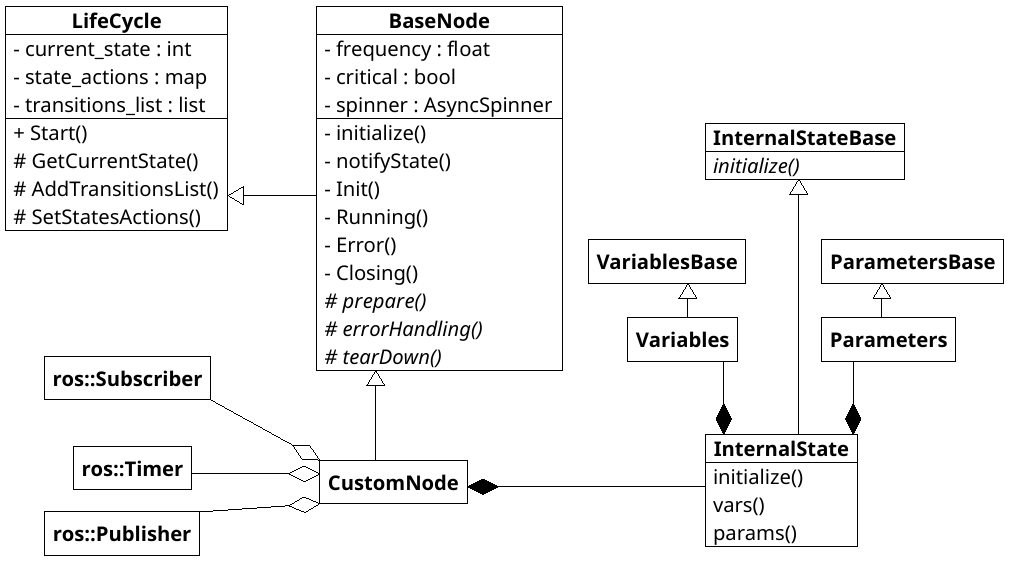
\includegraphics[width=\textwidth]{gfx/class}
    \caption{TODO}\label{fig:node-class}
\end{figure}

\section{Engineered ROS node}
\label{sec:ros-node}
Differently from other middleware or frameworks, ROS does not constrain the developer on the structure of the components; it was designed to be maximally flexible following the mantra: ``\textit{we don't wrap your main()}''. While this approach certainly contributed to the popularity and growth of ROS as a middleware and de facto standard for robotics, at the same time it created a very heterogeneous landscape for ROS nodes. Some of them are well designed, rich in functionalities, robust and configurable, others are cobbled together for a prototype and then used as legacy code for one single core functionality. Often this second category is created by experts in a specific field (\eg, vision, control, manipulation, \etc) that lack the necessary programming and software engineering skills and knowledge to develop a well-designed and robust node. With our approach we are targeting specifically this category of developers, that posses the expertise to contribute to the robotic community, but are discouraged by the programming required.

Since ROS does not impose any structure for the node, the simplest approach for automatic code generation would be to target an essential node, covering the minimum functionalities required to run it. There are few advantages in this approach: easier to implement code generator, simpler and more readable output, an implementation closer to what the developer knows. However, such a direct approach would have significant downsides: a lax relationship between the node and its model, lack of advanced functionalities that can be hidden in the automatic programming approach, less flexibility of the implemented node, more work left to the developer (\eg, testing, debugging, performance evaluation, \etc), more tampering by the developer with the basic structure of the node, no real benefit between a handcrafted and an automatically generated node. For all these reasons we decided to created an engineered base node that can be used as a reference and starting point for automatic code generation.

%TODO may not be simplified in the final version
Figure~\ref{fig:node-class} shows a simplified UML diagram of a custom node based on the engineered ROS node. Immediately, it is possible to recognise three main components: \textit{LifeCycle}, \textit{ROSNode}, and \textit{InternalState}. Each of them represent one of the main characteristics captured by the engineered node. The \textit{LifeCycle} implements an internal state machine that controls the evolution of the node. The \textit{ROSNode} is the core implementation of the node, capture all the ROS-related functionalities and management procedures. The \textit{InternalState} capture all the developer-defined parameters and variables necessary for the correct execution of the node.

\subsection{Life cycle}
When working with component-based approaches, it is important to define a recurring and consistent behaviour of the component, in the case of robotic components it is even more important, since they often operate with strict timing constraints and implement critical functionalities. In Section~\ref{sec:ros-in-aadl}, we presented how a life cycle of a node can be modelled in AADL, and how it can be used to guide the initialisation, configuration and execution of a component. To capture the same behaviour in the engineered node, we developed the \textit{LifeCycle} class to define the evolution of the node. While various implementations of state machines in C++ already exists, a very popular one has been around for almost 20 years\footnote{https://www.codeproject.com/Articles/1087619/State-Machine-Design-in-Cplusplus-2}, we opted to create a stripped down version that trades some functionalities for simplicity, understandability, and modern development approaches. The result is a very lightweight state machine, that supports dynamically defined states and transitions and it is completely ROS-independent.

To maintain the generality of the implementation, the class itself does not specify any state or transition. It only defines an empty enumeration that the subsequent classes can extend to define their own states. The valid transitions are defined as a list of pairs, going from one state to another, as for the states, the list is created by classes extending or using the state machine. The last initialisation step before running the state machine is to bind each state to a function. In practice, the binding is done by creating a map with the state as the key and a \texttt{std::fuction} as the value. Class template \texttt{std::function} is a general-purpose polymorphic function wrapper, it can be assigned to any callable target (\eg, functions, lambda expressions, pointers to member functions, \etc), this makes this approach particularly flexible and not bound to any specific implementation. When the initialisation is complete, the state machine can be started, the initial state is the one defined in the constructor, but there is no specific definition for a termination state. At each execution loop, first, the state machine execute the function bound to the specific state, then, it checks if there is a valid transition waiting to be performed, if there is one, the loop repeats and a new state-bound function is executed, otherwise the state machine has reached a final state and the execution terminates. While the list of all possible transitions is defined during the initialisation phase, each specific change of state is defined at runtime in all the state-bound functions. This is necessary, for example, to distinguish between a successful component initialisation that goes from an initial to a running state, to an unsuccessful one that would take the component to an error state. In practise, at the end of each state-bound function, the developer needs to specify the next state depending on the current outcome of the execution, then the state machine will check if the transition is valid (\ie, it is in the transitions list) and execute it. Mirroring the model presented in Section~\ref{sec:ros-in-aadl}, the engineered node supports five different states: initialisation, running, error report and closing. How they are implemented, what is their role and which ROS functionalities they evoke will be detailed in the next section.

\begin{figure}[t]
    \centering
    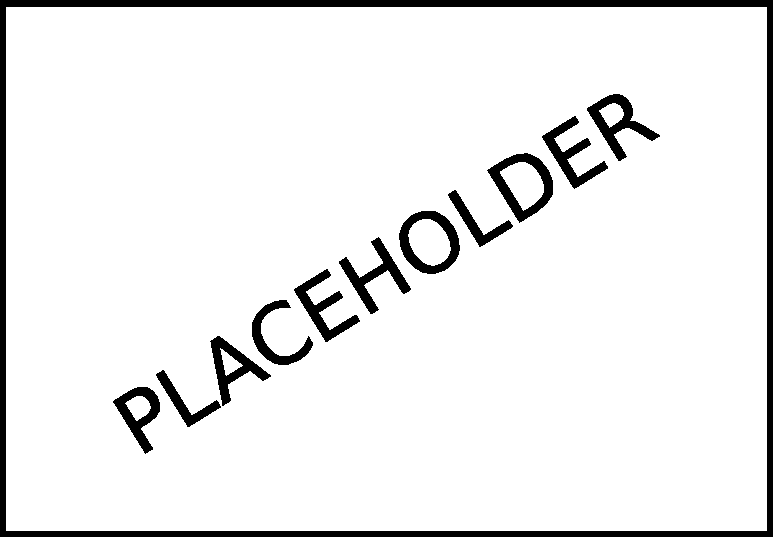
\includegraphics[width=0.8\textwidth]{gfx/placeholder}
    \caption{TODO}\label{fig:state-machine}
\end{figure}

\subsection{ROS node}
The core implementation of the engineered ROS node is in the \textit{ROSNode} class, here the life cycle is defined and materialised, and all the basic ROS-related functionalities are implemented. By defining this class, we can streamline the development process of a component by hiding the base initialisation procedure of a ROS node, create a well defined structure the developer can follow, and enhance the base implementation by adding additional functionalities (\eg, error detection and state report). The \textit{ROSNode} class extends directly the \textit{LifeCycle} class, therefore, the first implementation step is to define the states, the valid transitions and method bound to each state. Figure~\ref{fig:state-machine} presents the complete definition of the internal state machine, this mirrors the description provided in Section~\ref{sec:ros-in-aadl}. Each state is bound to a specific method of the class, and it implements a core functionality of the node.

\paragraph{Init} This method is bound to the initial state of the node (\ie, \texttt{ST\_INIT}). It is defined as a two-steps process and all the initialisation procedures of the component are implemented here.

The first step is a common initialisation that applies to every node, it sets up the ROS environment and defines the asynchronous spinner\footnote{http://wiki.ros.org/roscpp/Overview/Callbacks and Spinning}. In Section~\ref{sec:ros-in-aadl}, we modelled the ROS node with a external port to communicate the current state of the node after every transition, in this phase of the initialisation, the base node create the connection with the ROS service in charge of receiving this notifications. In ROS, a client can register to a service even if the server is not active, all the communications are lost until the service is finally started. This behaviour is not a problem for a status notification system, since it is meant to exist only to supervise the general evolution of the internal life cycle of the node. Nevertheless, our aim is to create a flexible base node that can adapt to different situations, thus, we defined an extra configuration property for the node, the developer can initialise the node as \textit{critical}. When a node is critical, instead of just starting the status notification service, the initialisation procedure will wait until the service is up, and then registers to it. In this way, an external supervisor node in charge of monitoring all the critical nodes can trace the entire evolution of their life cycles and act accordingly if something does not behave as expected. After the general initialisation procedure, the first action is to externally notify the state of the node, again the notification method itself behave in a different way for critical and non-critical nodes. To save bandwidth and reduce the number of requests, non-critical nodes notify their new state after a transition only if it is different from the previous one, in other words, they do not notify transitions on self-loops. Critical nodes are meant to be constantly monitored by the supervisor, therefore they notify their state after every transition, basically, in this case, self-loops are used as a way to measure the liveness of the node.

If the basic initialisation is completed successfully, the second step of the set up of the node is activated. An unsuccessful outcome is considered a critical failure and the node is instantly shut down. The second part of the initialisation is an abstract method not implemented in the \textit{ROSNode} class (\ie, the \textit{prepare} method) and it is meant to be used by the child class to define any node-specific initialization procedures. The developer can use this method to fill parameters and variables with their initial values, set up publishers and subscribers, or perform any other special initialisation (\eg, activate hardware connections, pre-fill data structures, \etc). If this preparation phase is completed successfully the method will trigger the transition to the main execution state. Differently from the base initialisation, an unsuccessful preparation phase will trigger a transition in error state. This is because we cannot anticipate what kind of procedure the developer will implement in this second part of the initialisation, therefore issues in this phase may be resolved in a specific error management procedure and lead to a successful initialisation.

\paragraph{Running} A complete and successful initialisation will transition the state machine in the \texttt{ST\_RUNNING} state, and this is the method bound to it. Since the engineered ROS node is built around an asynchronous spinner, most of the ROS-related functionalities (\ie, checking subscribers, services and timers) are executed in a separate thread, hence this method only needs to check for errors or node termination. When the node is working with no issues, the \textit{Running} method is just a low-frequency (\ie, 1 Hz) repeating self loop, two things can change this condition: first, one of the asynchronous activities (\eg, a subscriber callback) sets an error flag, or second, an external signal triggers the shutdown procedure. In the former case, this method interrupts its self loop and trigger a transition to the error state, in the latter, it receives the signal and changes the current state of the life cycle to shutdown. When the node is initialised as \textit{critical}, the behaviour of the \textit{Running} method does not change, however, the state notification happens at every self loop instead of only after the first transition. Given the fundamental functionalities implemented in this method, the developer cannot directly modify it, however it is possible to change the frequency of the self loop. Given the structure based on the asynchronous spinner, changing the frequency will not influence the behaviour of any ROS-related functionality, but it can change how fast the node reacts to errors or terminations; specifically, the higher the frequency the shortest will be the time between the generation of errors and interrupts and their detection. Changing the frequency of the self loop it is also useful to monitor the liveness of critical nodes. 

\paragraph{Closing} As any other process, ROS nodes can be closed by sending a termination signal (\ie, SIGINT). Normally, they already implement a handle to capture the signal and force a shutdown of the node, in the engineered node we replace it with our own version. Our handle does not perform any shutdown procedure, it just capture the signal and sets a flag; this flag will cause the \textit{Running} method to trigger a transition to the \texttt{ST\_CLOSING} state.  In this method bound to the state is where the actual shutdown procedure happens: first, it triggers a final state notification, so a potential supervisor knows that the node is shutting down, then it execute a custom \textit{tearDown} method, and finally it shuts down any ROS-related functionality. The \textit{tearDown} method is the shutdown counterpart of the \textit{prepare} method of the initialisation. It is abstract and not implemented in the base class, any child class extending \textit{ROSNode} will implement it with their own specific shutdown procedure. This is done to let the developers gracefully close existing connections (\eg, device drivers), propagate the shutdown to other nodes (\eg, critically dependant components), or provide additional shutdown notifications (\eg, specific logging systems). Since this is the terminal state of the life cycle, this method does not implement any transition.

\paragraph{Error} Natively, ROS does not provides any system to manage errors during the execution of the node. In our engineered node, we created an extensible structure to identify, detect and react to errors. The \textit{ROSNode} class defines an enumeration with few predefined error codes, they cover some common issue that may happen during the normal functioning of a node. They are:
\begin{itemize}
\item \texttt{PARAM\_ERROR}: this is a typical initialisation error, when a necessary parameter is not found in the parameter server. The node cannot run correctly when partially initialised, a way to handle this error is to wait until the parameter is available and then restart the initialisation procedure.
\item \texttt{SUB\_FAILED}: one of the subscribers of the node fails. This may compromise the entire node (\eg, set-point subscriber for a control node) or just disable one of its functionalities (\eg, a multiplexer missing one of the inputs). Depending on the situation this may or may not require the shutdown of the node. 
\item \texttt{PUB\_FAILED}: one of the publishers of the node fails. As for the subscribers, this may be very impactful (\eg, a planner that cannot publish the result) or a minor inconvenience (\eg, a visualisation topic not initialised), and therefore could prompt a shutdown of the node.
\item \texttt{INVALID\_MESSAGE}: This is an error that can be triggered during a subscriber callback or before publishing a message. A message has an unexpected value (\eg, negative distance, out of bound acceleration, empty path). Sometimes malformed messages are inconsequential, and the error handler will just record them, in other cases they can be hazardous and require to halt the node execution. 
\end{itemize}

These error codes are mostly related to the correct execution of ROS functionalities, on top of these, the developer can extend the enumeration and define his own error codes, to cover problem-related corner cases. 

At any moment during the normal execution of the node, the developer can use the \textit{faultDetected} method to notify one of the possible error codes. After the initialisation process or during the \textit{Running} self loop, if any error code is set, the system will transition to the  \texttt{ST\_ERROR} state. The \textit{Error} method is bound to this state, during its execution, first it notifies the state transition, to let any potential supervisor know that the node is in an error state, then it calls a method to handle the error, finally, after \textit{errorHandling} returns, if the error code is still set, the error is unsolvable and the node transition to the \texttt{ST\_CLOSING} state, otherwise, the node can go back to normal execution. The \textit{errorHandling} method is similar to the abstract method used during the initialisation and closing phases, as before, it is an abstract method that the developer can extend in the child class to manage any specifically defined error codes. Differently from the previous two, it is not a pure abstract method, since we provide a basic implementation in the \textit{ROSNode} class to manage the four already defined error codes. The developer can decide to reimplement completely the method (\eg, complex nodes with articulated initialisation procedures), run it alongside the existing one (\eg, few problem-related corner cases), or skip error management and leave only the already defined implementation (\eg, simple node requiring minimal definitions).

\subsection{Internal state}
Components are meant to be reusable through composition and parametrisation. The computation graph of ROS combined with our model-based approach ensure the composability, by providing deployment-time rewiring and decomposing components functionalities. On the contrary, parametrisation is not embedded in the design of the nodes. ROS provides various system-level tools to manage parameters: a centralised system to store and collect parameters (\ie, the parameter server), the corresponding APIs to fetch and set them, and a system to dynamically change parameters in real time. However, how to integrate them in the component is left to the developer. The result is parametrisation is often ignored or misused. Parameters are uncategorised and mixed between functionalities, modified during execution creating inconsistencies, defined conceptually but then hard-coded as constants in the implementation. This issues prompted us, originally, to exploit data modelling languages to capture the parametrisation of the component, and, in the engineered node, to design a separate class to encapsulate the parameters of the node.

Parameters are the external-facing part of the internal state of the component, they codify a specific configuration defined before execution; variables, on the opposite, are internal-facing, they evolve with the node and exist only in the time frame of its execution. As mentioned at the beginning of this section, ROS does not provide any structure to support the internal state of the node, in the case of the variables, it means there is no predefined way to safely store and share between callbacks the information extracted and derived from messages. Normally, there are two approaches used when developing ROS nodes, one is for traditional imperative implementations, where variables are declared as global and shared between callbacks, the other wrap the entire node in a class, it uses methods as callbacks and attributes for variables. While this approaches are not inherently wrong, they have significant downsides. They reduce the portability of the node design by removing the distinction between ROS-specific (\eg, declaration of publishers and subscribers) and problem-specific (\ie, the necessary logic to implement the functionalities of the node) implementations, they are harder to debug since they are not encapsulated and may have unpredictable side effects, they are more difficult to extend and modify since they do not present a common interface. Our solution is to create an overarching class encapsulating both parameters and variables, and present a single interface that the developer can use to access, modify, share and store the internal state of the component.

As visible from Figure~\ref{fig:node-class}, the internal state of the node is built using a hierarchical approach. The superclass is called \textit{InternalStateBase}, it has two members: a structure for variables of type \textit{VariablesBase} and a constant structure for parameters of type  \textit{ParametersBase}. Parameters are defined as constant, this means that after setting their values during the initialisation phase, it is guaranteed they will not change. An exception to this is when the node implements a dynamic reconfigure system, in this case there is a special callback in charge of managing the parameters and changing them according to an external control panel. In general, by defining the structure as constant it is possible to limit any modification of the parameters to specific procedures, and avoid unintentional modifications using compile-time checks. Both the parameters and variables structures are defined as shared pointers, this pointer-based declaration gives us the ability to treat each structure as a single entity, while, at the same time, avoiding useless and memory-consuming copies when accessing them in external procedures. The superclass has only one method, a pure abstract initialisation method that the developer has to implement in the child class; this is designed to force the developer to initialise all the parameters in the same location and to set an initial value to all the variables. To increase the flexibility of the base node, the internal state is not declared directly in the \textit{ROSNode} superclass, the developer can extend \textit{InternalStateBase} to create his own internal state class and declare it in the custom node. To better exploit the structure provided by the superclass, the developer can extend the parameters and variables structures, to define all the problem-specific details.

\section{Custom ROS node}
In Section~\ref{sec:ros-node}, we presented the engineered node as the starting point for the automatic programming process, however, the classes defined are perfectly suitable to be used directly by a developer to create their own node. In this section, we will present how a custom node can be implemented using the engineered node as a starting point, using the same approaches and structures the automatic code generator would create.

Since it is an independent class used by the rest of the node, the first step should be the definition of the internal state, and in that, the developer has to start from the definition of his own variables and parameters structures. Although the two base structures do not provide any functionality, it is ideal to extend them and exploit a polymorphic approach to define the internal state. The automatic code generator extends them and adds constructors to initialise the instances to their default, for parameters, and initial, for variables, values. The \textit{InitialStateBase} class exists to provide an unified interface between the node and its internal state, therefore, following the concepts of information hiding used in object-oriented programming, it is necessary to implement accessors for both parameters and variables. Since we are working with pure data structures declared as shared pointers, the most elegant approach is to define accessors for the entire structures and let the developer use directly the fields. To complete the definition of the internal state, it is necessary to implement the abstract initialisation method. A developer can create any complex initialisation, but in our automatic programming approach, we delegate the parameters set up to the core node functionality and use a copy constructor, while for the variables we invoke the constructor with no parameters defined in the structure.

After completing the definition of the internal state, a developer can move to the implementation of the node itself. The engineered node wraps all the main ROS-related functionalities in a single class, to implement the custom node the developer has to extend the \textit{ROSNode} base class. In the custom node class declaration three abstract methods are overridden from the superclass: \textit{prepare}, \textit{tearDown} and \textit{errorHandling}. Additionally, all the callbacks related to subscribers, services, timers and actions are defined as class methods. Since the class is the container of all the ROS-related code, the timer, publisher, subscriber, client, server and action objects are all declared as class members. Lastly, to complete the class definition, it is necessary to declare the internal state instance. These are all the methods and attributes that are necessary to implement the child class as an extension of the \textit{ROSNode} base class, and to cover all the fundamental ROS functionalities. When using the code generator only these methods and attributes will be automatically created, however, there is no restriction on the complexity of the class and a developer can declare all the additional helper methods and attributes necessary to ensure the proper functioning of the node.

As introduced in Section~\ref{sec:ros-node}, the \textit{prepare} method is meant to contain all the node-specific initialisation procedures. Here the code generator will create all the necessary calls to collect the parameters from the ROS parameter server and initialise the internal state of the node by setting the initial values of the variables. Moreover, callbacks of subscribers are initialised, publishers and services are advertised, and timers are set. At the end of this method, the node is ready and fully functional. Since it is abstract, the developer needs to implement the \textit{tearDown} method, here, all the necessary procedures to gracefully shutdown the node are executed. ROS manages all the connections transparently with respect to the end user, therefore, in a generic node there is no need for any particular shutdown procedure. If not specified otherwise in the model, the automatic code generator fills this method only with an output message to notify the system that the node is shutting down.  The last method that is necessary to implement to complete the definition of the child node as an extension of the base class is \textit{errorHandling}. All the structure to manage errors is not ROS-related and it is defined by us in the base class, since this is an extra functionality not necessary for the basic operation of the node, we already provide a simple handler that can be called directly and manages basic initialisation errors. However, if the developer wants to exploit the error management system, he can define his own error codes in the class by extending the enumeration defined in the \textit{ROSNode} superclass, and implements his own version of the \textit{errorHandling} method. Potentially, a developer could implements an extension of the internal life cycle of the node, where instead of a single error state there are multiple error states, each for a different category of problems. This can be done by extending state enumerator, binding new methods to the new states, and add all the necessary transition in the state machine. This is possible because by overriding the \textit{errorHandling} method, not only the developer can develop his own error management procedures, but he can change how the internal state machine evolves from the \texttt{ST\_ERROR} state. Without any specification in the model, the code generator will not override this method and use the implementation provided in the base class. While it is possible to specify in the model an implementation for the method itself, if the developer wants to change the life cycle of the node, he needs to do that by modify directly the source code, since the modifications are too radical and in depth to be managed by an automatic programming system.

The last step to complete the implementation of a custom node is to define the logic related to the subscribers, timers, or actions callbacks. As mentioned at the beginning of this section, all the callbacks are defined as methods of the child class; ROS already defines the signature for all the callbacks, hence the developer only needs to implement them. He can read parameters from the internal state and store the output of processing in the variables structure. Practically, there is no issue in implementing the logic directly in the callbacks, however, with our automatic programming approach we try to push as much as possible the separation between the problem-specific and the ROS-related implementation. The automatic code generator creates a function call for each callback using the structure defined in the model as a reference. The functions have access to the parameters and variables structures and to the message, but their entire implementation is completely independent from the node. This function can be used as a bridge between ROS and a domain-specific library and can be easily tested and debugged without the need of running the node. With the addition of the logic the implementation of the custom node is complete. Of course, since this is a C++ implementation, the developer needs to create all the necessary configuration files to build the executable. With the automatic programming approach, all the necessary file are generated, and the developer only needs to add additional sources that were not specified in the model.

\section{Two-steps code generation}
Now that we have completely defined the input, a complete model description defined in AADL following the meta-model presented in Chapter~\ref{ch:Modelling} combined with data modelled using ASN.1 or JSON schema, and the output, the engineered ROS component implementing advanced functionalities and a list of approaches to implement a custom node, we can describe all the necessary transformations to convert the collection of model to a working architecture. In our toolchain, we adopted a two-steps approach, first a model-to-model transformation that converts the  input AADL model to an intermediate XML-based representation, then a model-to-text transformation to automatically generate ROS-compatible C++ code.

While AADL is popular in some specific fields (\eg, space applications, automotive and embedded hardware), it is a niche language, therefore there are only few options in terms of tools and support. In particular, there is only one maintained and open-source AADL model processor that supports model checking, parsing and code generation: Ocarina. As presented in Section~TODO, Ocarina is written in Ada and provides multiple functionalities (\eg, parsing, model analysis, schedulability analysis, \etc), but mainly it is a parser and code generator. With its frontend/backend structure it separates the parsing and syntax analysis of the AALD model (\ie, frontend) from the code generation of a specific target (\ie, backend). This means that a developer could implement its own backend to exploit the parsing capability of Ocarina to create his own code generator. In theory, we could have used this approach to create directly a code generator completely implemented as a backend, but we decided to use Ocarina only to create an intermediate representation.

There are multiple reasons behind this choice. First of all, not only Ocarina is implemented in Ada, but is follows the Ravenscar profile, this is necessary because some of the code generation targets are certified for safety-critical hard real-time applications, therefore the toolchain itself needs the same certification. The Ravenscar profile imposes some restrictions on the already challenging Ada language, making the development and maintenance of a new backend a difficult and time-consuming task. By using an intermediate representation we can implement the most challenging part of the code generation (\ie, ROS source code) with our preferred approach. Additionally, using an XML-based language, that we called AAXML, creates an intermediate artefact that can be used as a starting point for code generation, but also as the output of a different AADL parser. Ocarina is an independent project that we do not control directly, therefore we cannot base our entire toolchain on a technological solution that could disappear or change drastically. Lastly, a two-steps approach makes the entire toolchain more flexible, for example to extend the code generator to support ROS2 or a different framework, or to include additional models (\eg, a specific language to describe the component behaviour). There is one final, more practical reason, to adopt a two-steps approach and instead of generating directly ROS/C++ code, Ocarina already implements a backend that uses XML as a target. Unfortunately, the existing XML backend is currently non functional and not maintained, it was developed as a low-priority approach in an effort to create a bridge between AADL and a possible XML-based representation. Nevertheless, we used it as a guideline to create our own backend from scratch.

\subsection{From AADL to AAXML}
This is the first step of the code generation approach, it is a model-to-model transformation, since the original structure of the AADL model is preserved but converted in an XML-based representation called AAXML. The Ocarina frontend provides two output that can be used by the backend: an abstract semantic tree, this guarantee correctness of the syntax and semantic of the model, and an instance tree, this is the result of the instantiation process; both of them are used by the backend. To implement the \textit{aaxml\_ros} backend, we followed the structure already established by Ocarina, with few modification to make the toolchain more suitable to the needs of a robotic system. First the backend needs to be registered to the frontend, so it can be called by the toolchain, after this simple initialisation phase, the automatic code generation process can start; it is a recursive approach that  analysing the root system of the model and goes through subcomponents, features, connections, and properties. In the default Ocarina implementation of a backend, only a single system can be parsed by the toolchain per call, but since in our model the hierarchy of AADL systems represents the deployment configuration of the architecture (\ie, launch files in ROS), we decided to modify the backend to parse all the root system component (\ie, system that are not subcomponents of other systems) to be able to generate all the necessary launch files at the same time.

\paragraph{components} As mentioned before, the code generation process is recursive, it always starts from a component. A component is mostly characterised by its subcomponents, ports and connection, however, few details can be extracted directly from it and converted to AAXML. The \textit{name}, an unique identifier of the actual instance of the component, necessary when there are duplicates coexisting in the same architecture. The \textit{type}, the reference to the specification of the component, depending on the level of specification it can be an interface or a complete definition. The \textit{category}, this attribute specify the AADL type (\eg, process, thread, system, \etc) associated with the component, it is guarantee to be compatible with the container component by the syntactic and semantic analysis done by the frontend. The \textit{namespace}, it specifies the package containing the component, while this seems a superfluous information, it is extremely important when referencing component not defined in the same package of the system. The subcomponents list, AADL has a hierarchical structure and Ocarina manages it using a recursive approach, this list is used to perform all the recursive call and complete the traversal of the tree.

Listing~\ref{lst:comp-aadl} shows a small example of a system containing a single process as subcomponent, this is the minimal AADL architecture that we can model and instantiate. In Listing~\ref{lst:comp-aaxml} presents the AAXML counterpart of the model, where the properties described are encoded in an XML-based format. In this minimal structure, no information is lost when converting the model from AADL to AAXML.

\begin{lstlisting}[frame=tb,caption={TODO caption},label=lst:comp-aadl]
system root_system
end root_system;

system implementation root_system.impl
  subcomponents
  main_process: process custom_process.impl;
end root_system.impl;
\end{lstlisting}

\begin{lstlisting}[frame=tb,caption={TODO caption},label=lst:comp-aaxml]
<system>
	<type>root_system.impl</type>
	<category>system</category>
	<namespace>aadl_xml</namespace>
	<subcomponents>
		<component>
			<name>main_process</name>
			<type>custom_process.impl</type>
			<category>process</category>
			<namespace>aadl_xml</namespace>
		</component>
	</subcomponents>
</system>
\end{lstlisting}

\paragraph{Features} The subcomponents list is one of the defining characteristics of a component, the other is the set of features. They define the frontier between the component and the external environment, moreover, when working with interface-only definitions (\eg, existing ROS nodes), they are the only element characterising the component. For these reasons it is important to capture all the necessary information when converting the model from AADL to AAXML. Features have a list of characteristics that are mandatory and are necessary to specify them, and others that optional. First of all, it is necessary to identify the type of feature, AADL categorises them in two main groups: accesses (\ie, subprogram, data and bus) and ports (\ie, data, event and event data); this is captured by the \textit{category} tag. By defining the \textit{type} it is possible to specify the specific subcategory of a port (\eg, \textit{event\_data}), for accesses there is no need for specialisation since the component they are connected to determinates their  specific subcategory. Another attribute that is unique to ports and not necessary for accesses is the \textit{direction}, since ports can define a specific ingoing, outgoing or bidirectional communication. While in the model it is necessary to specify if a feature provides or requires access, this specification can be dropped in this conversion since it is important only to define the topology of the architecture, which is already checked by the frontend. This covers all the mandatory definitions for a feature, additionally, it is possible to specify the data type of the feature. Since the data is a component, we need two information to identify it: the package and the type. While subprogram and bus accesses target a subprogram or bus instead of a data component, the procedure is the same since they are identified by their type and package.

Listing~\ref{lst:feature-aadl} show the interface model of the component included in the system presented in Listing~\ref{lst:comp-aadl}. It defines a single event data port exchanging messages with a specific data type. Given this definition the AAXML file can be extended as shown in Listing~\ref{lst:feature-aaxml}, the \textit{features} tag is a child of the \textit{component} tag, while this replicates the feature information in multiple places in the file, it also streamlines the code generation process in the next phase.

\begin{lstlisting}[frame=tb,caption={TODO caption},label=lst:feature-aadl]
process custom_process
	features
		a_port: out event data port pkg::some_data;
end custom_process;
\end{lstlisting}

\begin{lstlisting}[frame=tb,caption={TODO caption},label=lst:feature-aaxml]
<component>
	[...]
	<features>
		<feature>
			<name>a_port</name>
			<direction>out</direction>
			<type>event_data</type>
			<datatype>some_data</datatype>
			<datatype_namespace>pkg</datatype_namespace>
			<category>K_PORT_SPEC_INSTANCE</category>
		<feature>
	<features>
</component>
\end{lstlisting}

\paragraph{connections} When dealing with connections we move outside the scope of a single component and we have to consider the interaction of multiple objects. For this reason, connections are defined, both in AADL and in AAXML, in the container, and they can connect two components in the same subcomponents set or a component and a frontier feature (\ie, a feature defined on the frontier of the container component). First, there is a list of characteristics referring directly to the connection itself. The \textit{name}, an unique identifier of the connection. The \textit{kind}, a mapping in AAXML of the original Ada node kind, currently the only possible value is \texttt{K\_CONNECTION\_INSTANCE}, however, we decided to include it in the AAXML file to support future extensions. The \textit{category}, as for features, connections may involve ports or accesses, this property specifies the type of the connection, it can be: \texttt{CT\_PORT\_CONNECTION}, for connection between two ports, \texttt{CT\_ACCESS\_DATA}, when connecting an access to a data component, or \texttt{CT\_ACCESS\_SUBPROGRAM}, when modelling a connection representing a remote subprogram call. Since connections are meant to describe the interaction between component, they carry information related to both components at the limits of the connection. Each description has a subsection called \textit{port\_info}, it includes the name of the source and the destination features, and the name and the type of the parent components.

Listing~\ref{lst:con-aadl} shows the modelling of the implementation of a system where two processes are connected, one with an output port and the other with an input port. Listing~\ref{lst:con-aaxml} presents how this connection is mapped on the AAXML file, since the system is the root of the hierarchy, the \textit{connections} tag is defined directly as a child of the root \textit{system} tag.

\begin{lstlisting}[frame=tb,caption={TODO caption},label=lst:con-aadl]
system implementation root_system.impl
	subcomponents
		cmpA: process pkg::processA;
		cmpB: process processB.impl;
	connections
		con1: port cmpA.out -> cmpB.in;
end root_system.impl;
\end{lstlisting}

\begin{lstlisting}[frame=tb,caption={TODO caption},label=lst:con-aaxml]
<system>
	[...]
	<connections>
	<connection>
		<name>con1</name>
		<kind>K_CONNECTION_INSTANCE</kind>
		<category>CT_PORT_CONNECTION</category>
		<port_info>
			<source>out</source>
			<dest>in</dest>
			<parent_source>processA</parent_source>
			<parent_source_name>cmpA</parent_source_name>
			<parent_dest>processB.impl</parent_dest>
			<parent_dest_name>cmpB</parent_dest_name>
		</port_info>
	</connection>
	</connections>
</system>
\end{lstlisting}

\paragraph{properties} In AADL, properties can be applied to every element in the model, moreover, in the definition of our meta-model, we introduced their importance in specifying components. Properties are such an important element of the languages, that additionally to all the already existing definitions, the designer can define his own set of new properties. Given their ubiquitousness, each AADL category has a set of general properties, plus specific ones, plus all the custom defined, the process of adding them to the AAXML file can happen at every point during the parsing of the tree. All properties defined in the model have at least two fields: the \textit{name}, the unique identifier of the property as defined in the language definition or in the property set, and the \textit{value}, the actual value of the property assigned by the designer in the specific instance of the model. Each property has a type (\eg, number, string, \etc), that is checked by the frontend for consistency but not replicated in the AAXML file, additionally, in AADL it is possible to define the measurement unit of a specific property, if present, it is included in the translated model using the \textit{unit} tag. Default (\eg, \textit{Period}) and custom (\eg, the \textit{Default\_name} of a topic) properties are managed in the same way, with the exception of the name of the property set containing the custom defined properties; it is included in the AAXML file using the \textit{namespace} tag. In AADL it is possible to set properties at any point in the model, this means that in the property section of a component it is possible to reference every property of its internal parts (\eg, features, connection, subcomponents,\etc) or, through dot notation, all the properties of the subcomponents. However, in AAXML, properties are defined in as direct children of the element owning them.

Listing~\ref{lst:pro-aadl} shows a definition of the implementation of a process component, it has a thread as a subcomponent and this thread has an output port on his frontier. As said before, it is possible, in the properties section of the process to specify both the properties of the subcomponent (\ie, \textit{Period}) and of the feature (\ie, \textit{Queue\_size}). Listing~\ref{lst:pro-aaxml} presents a portion of the AAXML file modelling the properties, while they were defined in the property section of the process, the \textit{component} tag in the listing references the thread, since it is the owner of both the feature and the \textit{Period} property. 

\begin{lstlisting}[frame=tb,caption={TODO caption},label=lst:pro-aadl]
process implementation componentA.impl
	[...]
	properties
		Queue_size => 1 applies to threadA.out;
		Period => 50 ms applies to threadA;
end componentA.impl;
\end{lstlisting}

\begin{lstlisting}[frame=tb,caption={TODO caption},label=lst:pro-aaxml]
<component>
	[...]
	<features><feature>
	<properties><property>
		<name>Queue_size</name>
		<value>1</value>
	</property></properties>
	</feature></features>
	<properties><property>
		<name>Period</name>
		<value>50</value>
		<unit>ms</unit>
	</property></properties>
</component>
\end{lstlisting}

\subsection{From AAXML to ROS/C++}
\label{sec:xml-cpp}
The second step of the code generation is a model-to-text transformation. Differently from the first step where the original AADL model was converted in a different format, here multiple models (\ie, AADL and ANS.1 or JSON schema) are combined to create code artefacts. In particular, the output of the code generation after this step will be a single ROS package that contains all the custom messages, services and actions (if they exists), the source code of all the nodes modelled combined with any already existing problem-specific implementation, all the necessary build and configuration files, and the launch files matching the deployment configuration specified in the model.





\textcolor{red}{
The code generator discussed in this work, takes the AAXML model produced by the customised back-end as input and translates it into a working ROS C++ environment, i.e., a set of one or more ROS packages equipped with all the necessary configuration files for compiling (e.g., the \textit{CMakeLists.txt} and \textit{package.xml} files, the custom messages and services, launch files, etc.). Each one of these packages also includes a programmatic list of all method interfaces declared by the developer within the model, making the output code application-specific.}

%We introduced two steps in our toolchain to exploit the already available XML parsers. 
The code generation module was developed entirely in Python 3, hence exploiting the \textit{lxml}~\cite{lxml} pythonic binding for the C libraries \textit{libxml2} and \textit{libxslt} (also integrating the XPath syntax~\cite{websiteXPath}), as XML Manipulation Toolkit.

For designing this code generator, we followed a Russian doll pattern, where elements call each others in chain until the final code is generated, as shown in Figure~\ref{fig:codegenerator-russiandollpattern}.

Each element in C++ to be generated has its own managing class in Python. For example, a variable in C++ is managed by a Python class which contains all the elements and the methods to represent the functionalities and properties of that C++ variable. The same goes for a C++ method, where a specific Python class manages it. Since a method can have variables as input, the corresponding managing Python class can contain an instance of the Python class dedicated to variables. Each of these variables has a specific type, which is managed by the \textit{type} class. When generating the C++ method code, the input parameter objects are triggered to generate their own code and together they cooperate to produce the complete method code.  Figure~\ref{fig:codegenerator-russiandollpattern} shows this exact example.

The entire code generation workflow is detailed throughout the remainder of this Section, accompanying each description with graph visuals.
%We will now go through the entire structure of the code generator detailing the code generator normal flow, summarizing with graphs the entire procedure.

\paragraph{Initialisation} The initialisation phase consists of some basic set-up instructions and the top-down reading of the AAXML tree. We used the \textit{XMLTags} module in Python for reading the tree, exposing all the AAXML tags produced by the Ocarina backend \textit{aadl\_aaxml} as a result. %Any change to the used tags in the first step of the toolchain is automatically reflected to the second step.
To accommodate for the main structure of AADL models being a \textit{system}, we also incorporated a \textit{SystemsManager} class in our code generator, to manage all the AADL \textit{system-level} components, represented instances of the Python \textit{System} class.

\paragraph{The System Loop} In AADL it is possible to define additional systems as system subcomponents. As a result, the code inspection and generation routine had to keep this factor into account. After the main system root (i.e., the outermost container) is retrieved, subsystems are lined up in a loop queue of type FIFO (i.e., First In First Out). Figure~\ref{fig:codegenerator-systemsloop} demonstrates how a \textbf{system loop} is formed: each highlighted block is the main actor of the following phases, where each system is analyzed and its code generated.
%This has to be treated accordingly by running the full code inspection and generation also over it; this chain can be as deep as one wants. 
%After gathering the main system root, namely the outer system, a loop queue is instantiated where new systems are added at the end, the already queued are popped one by one and examined. 
%This \textbf{system loop}. is shown visually in Fig.: the block highlighted is the main actor of the following phases, where each system is analyzed and its code generated.

\paragraph{Code Generation} The code generation process summarised in Figure \ref{fig:codegenerator-systemsloop} is quite straightforward. First, a new \textit{System} object is created, with all information relative to the current analyzed system (i.e., also including the launch file and the \textit{CMakeLists.txt} file ultimately required to compile and run the generated nodes). Both files are consistently updated by the code generator as the process goes on, this is necessary, since crucial information to be inserted these files (e.g., adding library dependency to ROS \textit{tf}) may only appear later in the code generation process.

Then, all the AADL processes in the \textit{system} are visited one at a time, in search for specific thread components that trigger the start of code generation. As thread components are identified by their type and, in this phase, a RegEx check is used to look for the target Python class matching the detected thread type. If a thread type is not recognised, it will simply be ignored and skipped by the code generator. In fact, in an AADL \textit{process}, threads can be associated to known types or marked as 'unknown'. This implementation strategy allows for the code generator to only look for supported parts, without limiting the completeness and expressive power of the input model. This may happen, for example, when modelling a sensor driver, which does not use publishers or subscribers to communicate with the hardware, but unique approaches, not identifiable by the code generator.

The currently supported thread types are six, reflecting the custom functionalities introduced in Section \ref{sec:transformation-rules}:
\begin{itemize}
\item{ \textbf{main\_loop.impl} identifies the main thread behind every single node. A node without this thread cannot work and it is skipped by the code generator.}
\item {\textbf{publisher.impl} identifies a thread with publishing capabilities. It is a generalised description, that needs some configuration parameters (e.g., message type, rate, topic name) to work properly and also a connection to specify where to send the published message.}
\item \textbf{callback.impl} is related to subscriber threads. As for its counterpart that publishes messages, a \textit{callback.impl} thread needs configuration parameters (e.g., message type, topic name) to be functional.
\item the \textbf{call\_pub.impl} thread receives a message in input and re-publishes it with some modifications. In a sense, it merges subscriber and publisher functionalities in one place.
\item \textbf{service\_provider.impl} indicates that the considered thread provides a service functionality
\item \textbf{timer.impl}, is the identifier used for threads that implement only timers and their callbacks.
\end{itemize}

%At this stage, the code generator starts looking for the known thread types and generates the relative code. 
The main thread is a required component for the process not to be ignored by the code generator. After the main thread is detected, the module analyses all the remaining threads. As flexibility is a requirement for future extension to new thread types, the thread libraries (i.e. the python classes \textit{Publisher}, \textit{MainThread}, \textit{Timer}) are imported at runtime only if used. This was achieved through the Python module \textit{importlib}. Defining and supporting a new thread type becomes then extremely easy and is done by simply extending the base class \textit{AADLThread} (which implements all said functionalities) and by adding an additional regular expression to map the newly-created class to its related thread type.

After all systems have been parsed and the queue is empty, the saving routine starts. In this phase, the launch file created at the very beginning is finally populated. Then, each node is saved and its executable name added to the \textit{CMakeLists.txt}, calling the instance of class \textit{CMakeLists} that manages it. Since the same node design can be reused inside the model, nodes sharing the same design, but with different functionalities, are generated. To overcome the problem of linking the correct node source to the node name in the launch file, after the node source is actually generated and saved, the equivalent entry in the launch file is updated if necessary. After the nodes and all their universe have been generated, it is the turn of custom messages and services.

\paragraph{Custom Messages And Services} In ROS it is possible to define a new custom message that relies on basic datatypes or on already existing ROS messages, and the same applies to services. To take advantage of these functionalities, we used a data modelling language called ASN.1. ASN.1 is an interface description language used to define data structures which can be easily serialised and deserialized. The code generator, is thus able to read and parse an ASN.1 description and to produce a working representation of a custom message or service, ensuring it is ROS-compatible. In ROS, message-only packages may exist, the code generator cover this case by creating the relative relative package with the \textit{CMakeLists.txt} during custom messages generation.

\subsection{Use Case: Publisher - Subscriber Example} \label{sec:use-case}

This section demonstrates a real use case of the customised Ocarina backend \textit{aadl\_aaxml} and code generator, when applied to a simple publisher-subscriber architecture. %The goal is to demonstrate that our toolchain is able to produce a good quality code.
We firstly introduce the publisher-subscriber model to then analyse its correspondence with the generated ROS package. To make the example more complete, we include the exchange of a custom message between the two nodes.

The AADL model represented in Listing~\ref{snippet:aadl_pub_sub_system}, shows a main system is called \textit{container} and its containing package \textit{pub\_sub}. Note that the latter package name will be reused as ROS package name. 
We refrain from reiterating all relevant definitions already introduced in Section~\ref{sec:background}, and discuss only the \textit{properties} associated to publisher-subscriber connection. Broadly, the publisher and the subscriber need to exchange messages on the same topic, where topics are identified by their name, e.g.,  \textit{``/pubsub"} in this case. The topic name is attached to the existing connection between the two, or, in other words, defined at the system level. In fact, placeholders for the topic should be specified within the process rather than as part of any other component of the system, in order to produce a functioning node.

% \begin{figure}[t]
% \centering
% 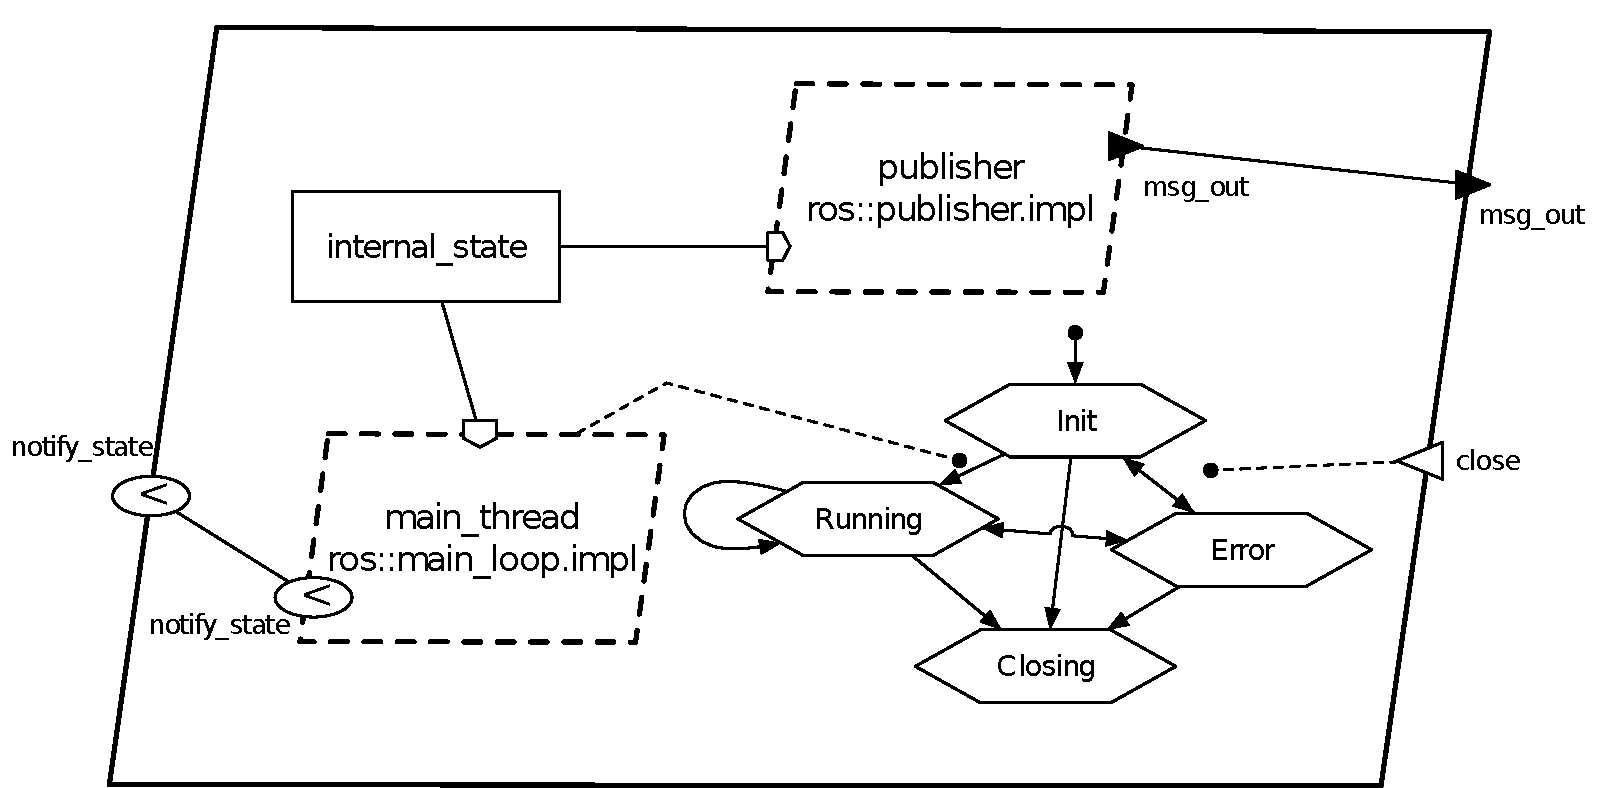
\includegraphics[width=0.95\hsize]{usecase-publisher}
% \caption{\label{fig:usecase-publisher}AADL graphical representation of a node including a publisher functionality (\textit{thread}).}
% \end{figure}

% \begin{figure}[t]
% \centering
% 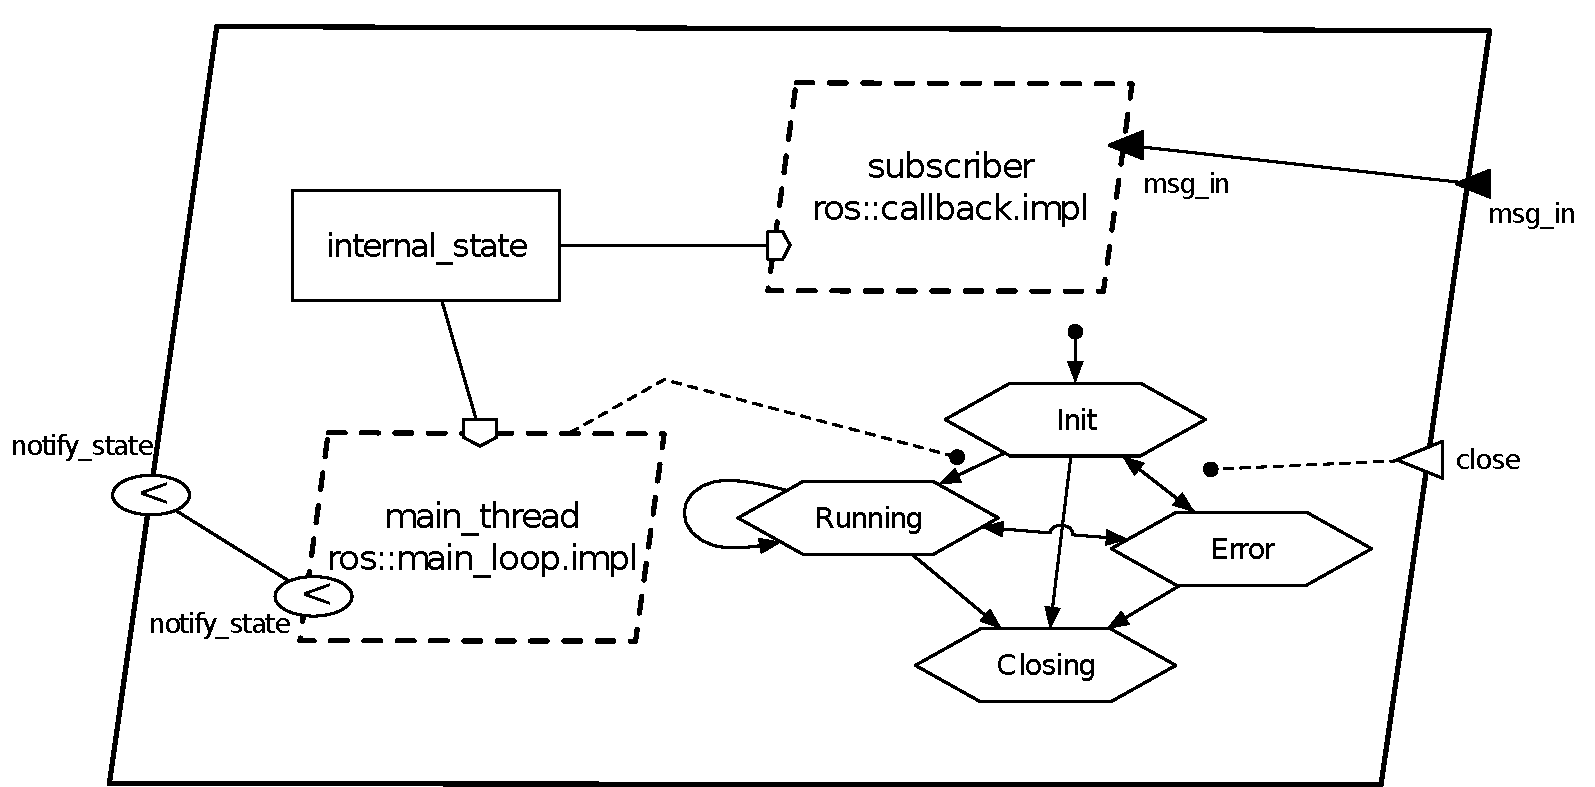
\includegraphics[width=0.9\hsize]{usecase-subscriber}
% \caption{\label{fig:usecase-subscriber}AADL graphical representation of how a \textit{process} (node) including a subscriber \textit{thread} (functionality) looks like.}
% \end{figure}

In Fig.~\ref{fig:usecase-publisher} and Fig.~\ref{fig:usecase-subscriber} are represented, respectively, the publisher and the subscriber models, except for their \textit{properties}. In both cases we have the following \textit{properties}:
\begin{itemize}
\item \textit{Source\_Text} and \textit{Source\_Name}: the first identifies the file where the application specific code will be placed, while the second represents the name of the function that will be called. In the publisher case, this function will return the message to be sent, while, for the subscriber, it will have as input the received message to be processed.
\item \textit{topic\_properties::Default\_Name}: it is the topic name placeholder in order to generate correctly the node. It can be different for the publisher and the subscriber, since the binding between them is done at system’s connections level and it is represent as a \textit{remap} in the ROS launch file.
\end{itemize}

Moreover, the publisher has a specific property, called \textit{Period}, where the frequency of the publisher is defined. The subscriber also has its own specific property called \textit{Queue\_size}, representing the maximum size of the subscriber message buffer.

Models in Fig.~\ref{fig:usecase-publisher} and Fig.~\ref{fig:usecase-subscriber} have the mandatory main thread implementation; it is important to see that the two threads inside the process, namely \textit{main\_thread} and \textit{publisher} or \textit{subscriber}, need to have their ports connected to the process’ ports, thus, at \textit{process} level, we have \textit{connections} and \textit{features} definitions.

In addition, the two figures show the common base model under each node. As stated in in~\cite{Bardaro2017}, the model of the base node contains a state machine, with four different states: \textit{init}, \textit{running}, \textit{closing} and \textit{error}. In AADL, each transition has to be triggered by an event; an event data port on the process models any external signal to force the shutdown of the node (i.e. SIGINT signal) and various ports on the main thread trigger the transition from a state to another. The current node state is saved \textit{data} element called \textit{internal\_state}. For each existing element of the model (i.e. threads, subprograms, connections, ports, etc.) it is possible to define in which state they are active, and this defines a specific workflow and a strict initialization procedure of the node.

In Listing~\ref{snippet:aadl_pub_sub_publisher} we present the code only for the publisher, but extending the same concepts can be easily extended the subscriber case:

\begin{lstlisting}[frame=tb,caption={AADL model for a simple process (node) implementing a publisher feature},label=snippet:aadl_pub_sub_publisher]
process talker extends ros::node
	features
 		msg_out: out data port custom_msgs::Complex;
end talker;

process implementation talker.impl extends ros::node.impl
 	subcomponents
 		publisher: thread ros::publisher.impl (message => data custom_msgs::Complex);
 	connections
 		chatter: port publisher.msg -> msg_out;
 	properties
 		Source_Text => ("Publisher.h") applies to publisher.function;
 		Source_Name => "publisher_function" applies to publisher.function;
 		topic_properties::Default_Name => "/out_topic" applies to msg_out;
 		Period => 10 ms applies to publisher;
 end talker.impl;
 \end{lstlisting}

The above example includes all the already cited components, as well as the thread output port, connected to the process port and the associated properties. It may be worth taking a closer look at how the datatype of the exchanged message is actually defined: the type is associated to the process output port and specified as a prototype of the thread. This ensures the thread type to match the process-level type.
In our example, the message is of \textit{Complex} type defined inside the package \textit{custom\_msgs}. Its definition is shown in Listing~\ref{lst:aadl_custom_msgs}. However, the actual implementation of said definition is enclosed in the \textit{``custom\_msg.asn''} linked file, in ASN.1 language.

\begin{lstlisting}[frame=tb,caption={AADL representation of a custom message},label=lst:aadl_custom_msgs]
data Complex
 	properties
 		Source_Text => ("custom_msg.asn");
end Complex;
\end{lstlisting}


Based on this model, the ROS packages generated by our toolchain have the following structure:
% \begin{itemize}

% \item[] 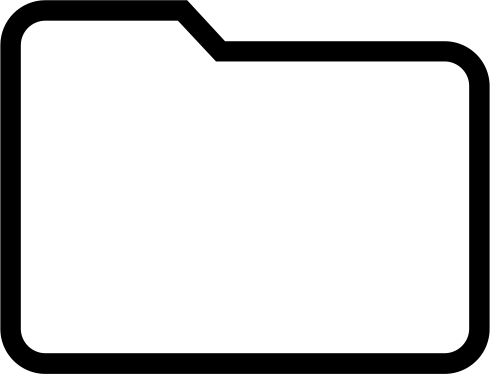
\includegraphics[width=0.3cm]{folder.png} pubsub
% \begin{itemize}
% \item[] 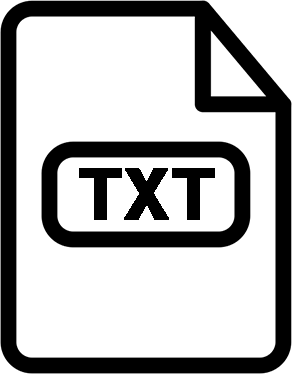
\includegraphics[width=0.3cm]{file_txt.png} CMakeLists.txt

% \item[] 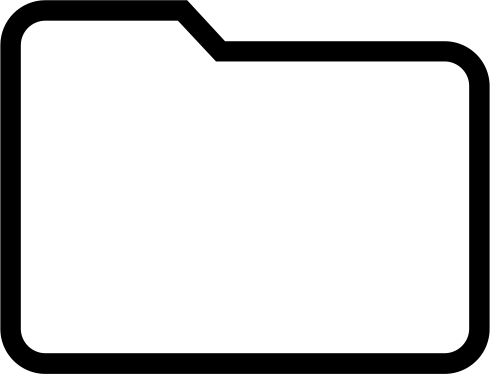
\includegraphics[width=0.3cm]{folder.png} include
% \begin{itemize}
% \item[] 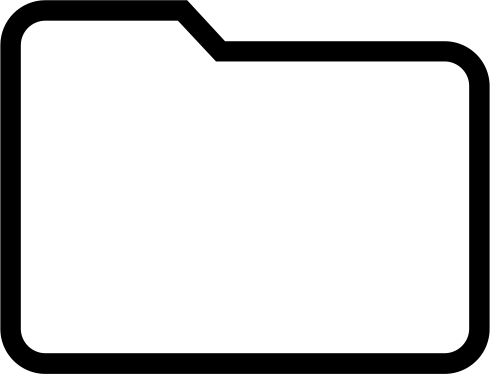
\includegraphics[width=0.3cm]{folder.png} pubsub
% \begin{itemize}
% \item[] 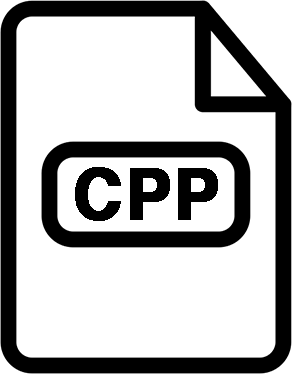
\includegraphics[width=0.3cm]{file_cpp.png} Publisher.h
% \item[] 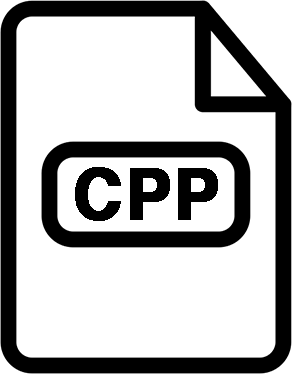
\includegraphics[width=0.3cm]{file_cpp.png} Subscriber.h
% \end{itemize}
% \end{itemize}

% \item[] 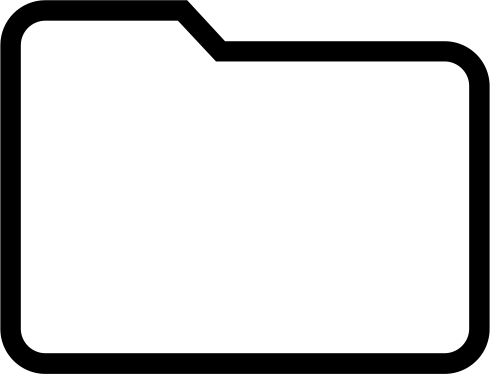
\includegraphics[width=0.3cm]{folder.png} launch
% \begin{itemize}
% \item[] 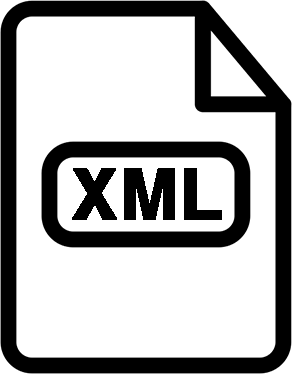
\includegraphics[width=0.3cm]{file_xml.png} container.impl.launch
% \end{itemize}

% \item[] 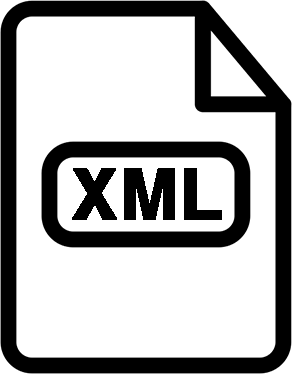
\includegraphics[width=0.3cm]{file_xml.png} package.xml

% \item[] 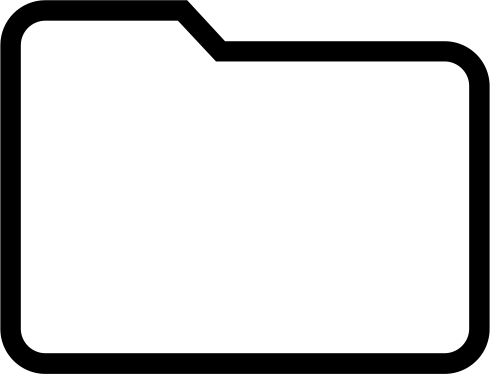
\includegraphics[width=0.3cm]{folder.png} src
% \begin{itemize}
% \item[] 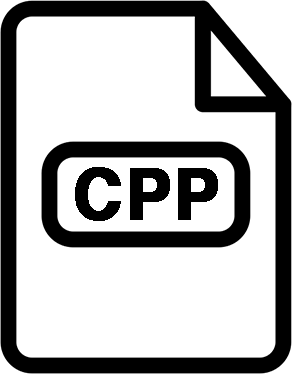
\includegraphics[width=0.3cm]{file_cpp.png} Publisher.cpp
% \item[] 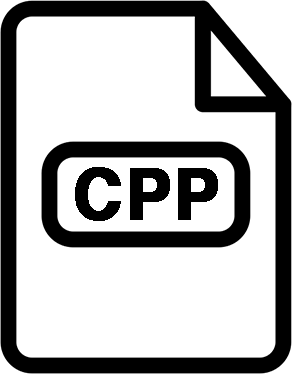
\includegraphics[width=0.3cm]{file_cpp.png} Subscriber.cpp
% \end{itemize}

% \end{itemize}

% \item[] 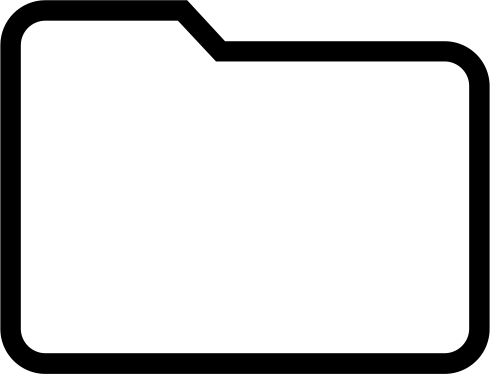
\includegraphics[width=0.3cm]{folder.png} custom\_msgs
% \begin{itemize}
% \item[] 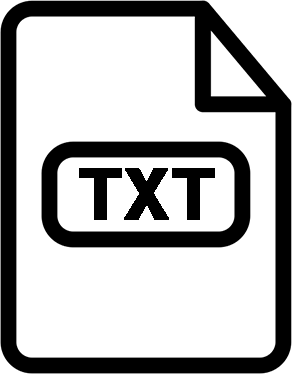
\includegraphics[width=0.3cm]{file_txt.png} CMakeLists.txt

% \item[] 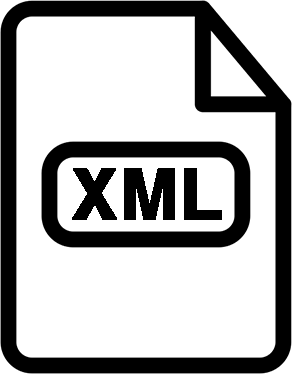
\includegraphics[width=0.3cm]{file_xml.png} package.xml

% \item[] 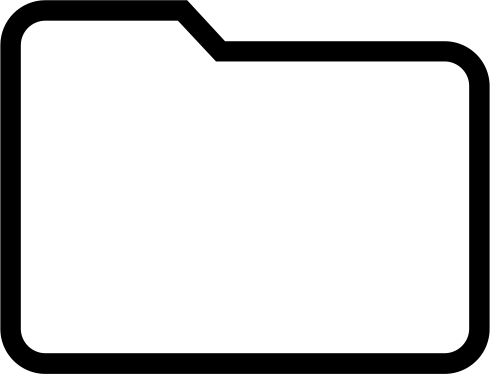
\includegraphics[width=0.3cm]{folder.png} msg
% \begin{itemize}
% \item[] 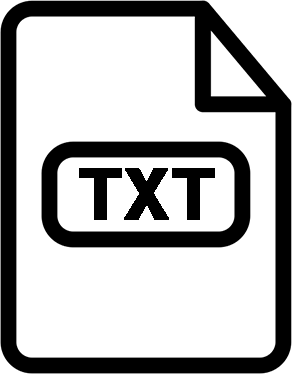
\includegraphics[width=0.3cm]{file_txt.png} Complex.msg
% \end{itemize}

% \end{itemize}
% \end{itemize}

\textit{Publisher.h} and \textit{subscriber.h} can be used as a guideline to implement the application-specific interface. The provided files, already import all the necessary libraries. Further, it is also important to note that decoupling these files from the rest of the ROS nodes, allows developers to test the implemented functions without launching the whole ROS environment at each iteration. This feature 
% simplifies both the developing and testing phases significantly, reducing the computational complexity of the underlying code.


%TODO update this figure to include the GSM
\begin{figure}[t]
\centering
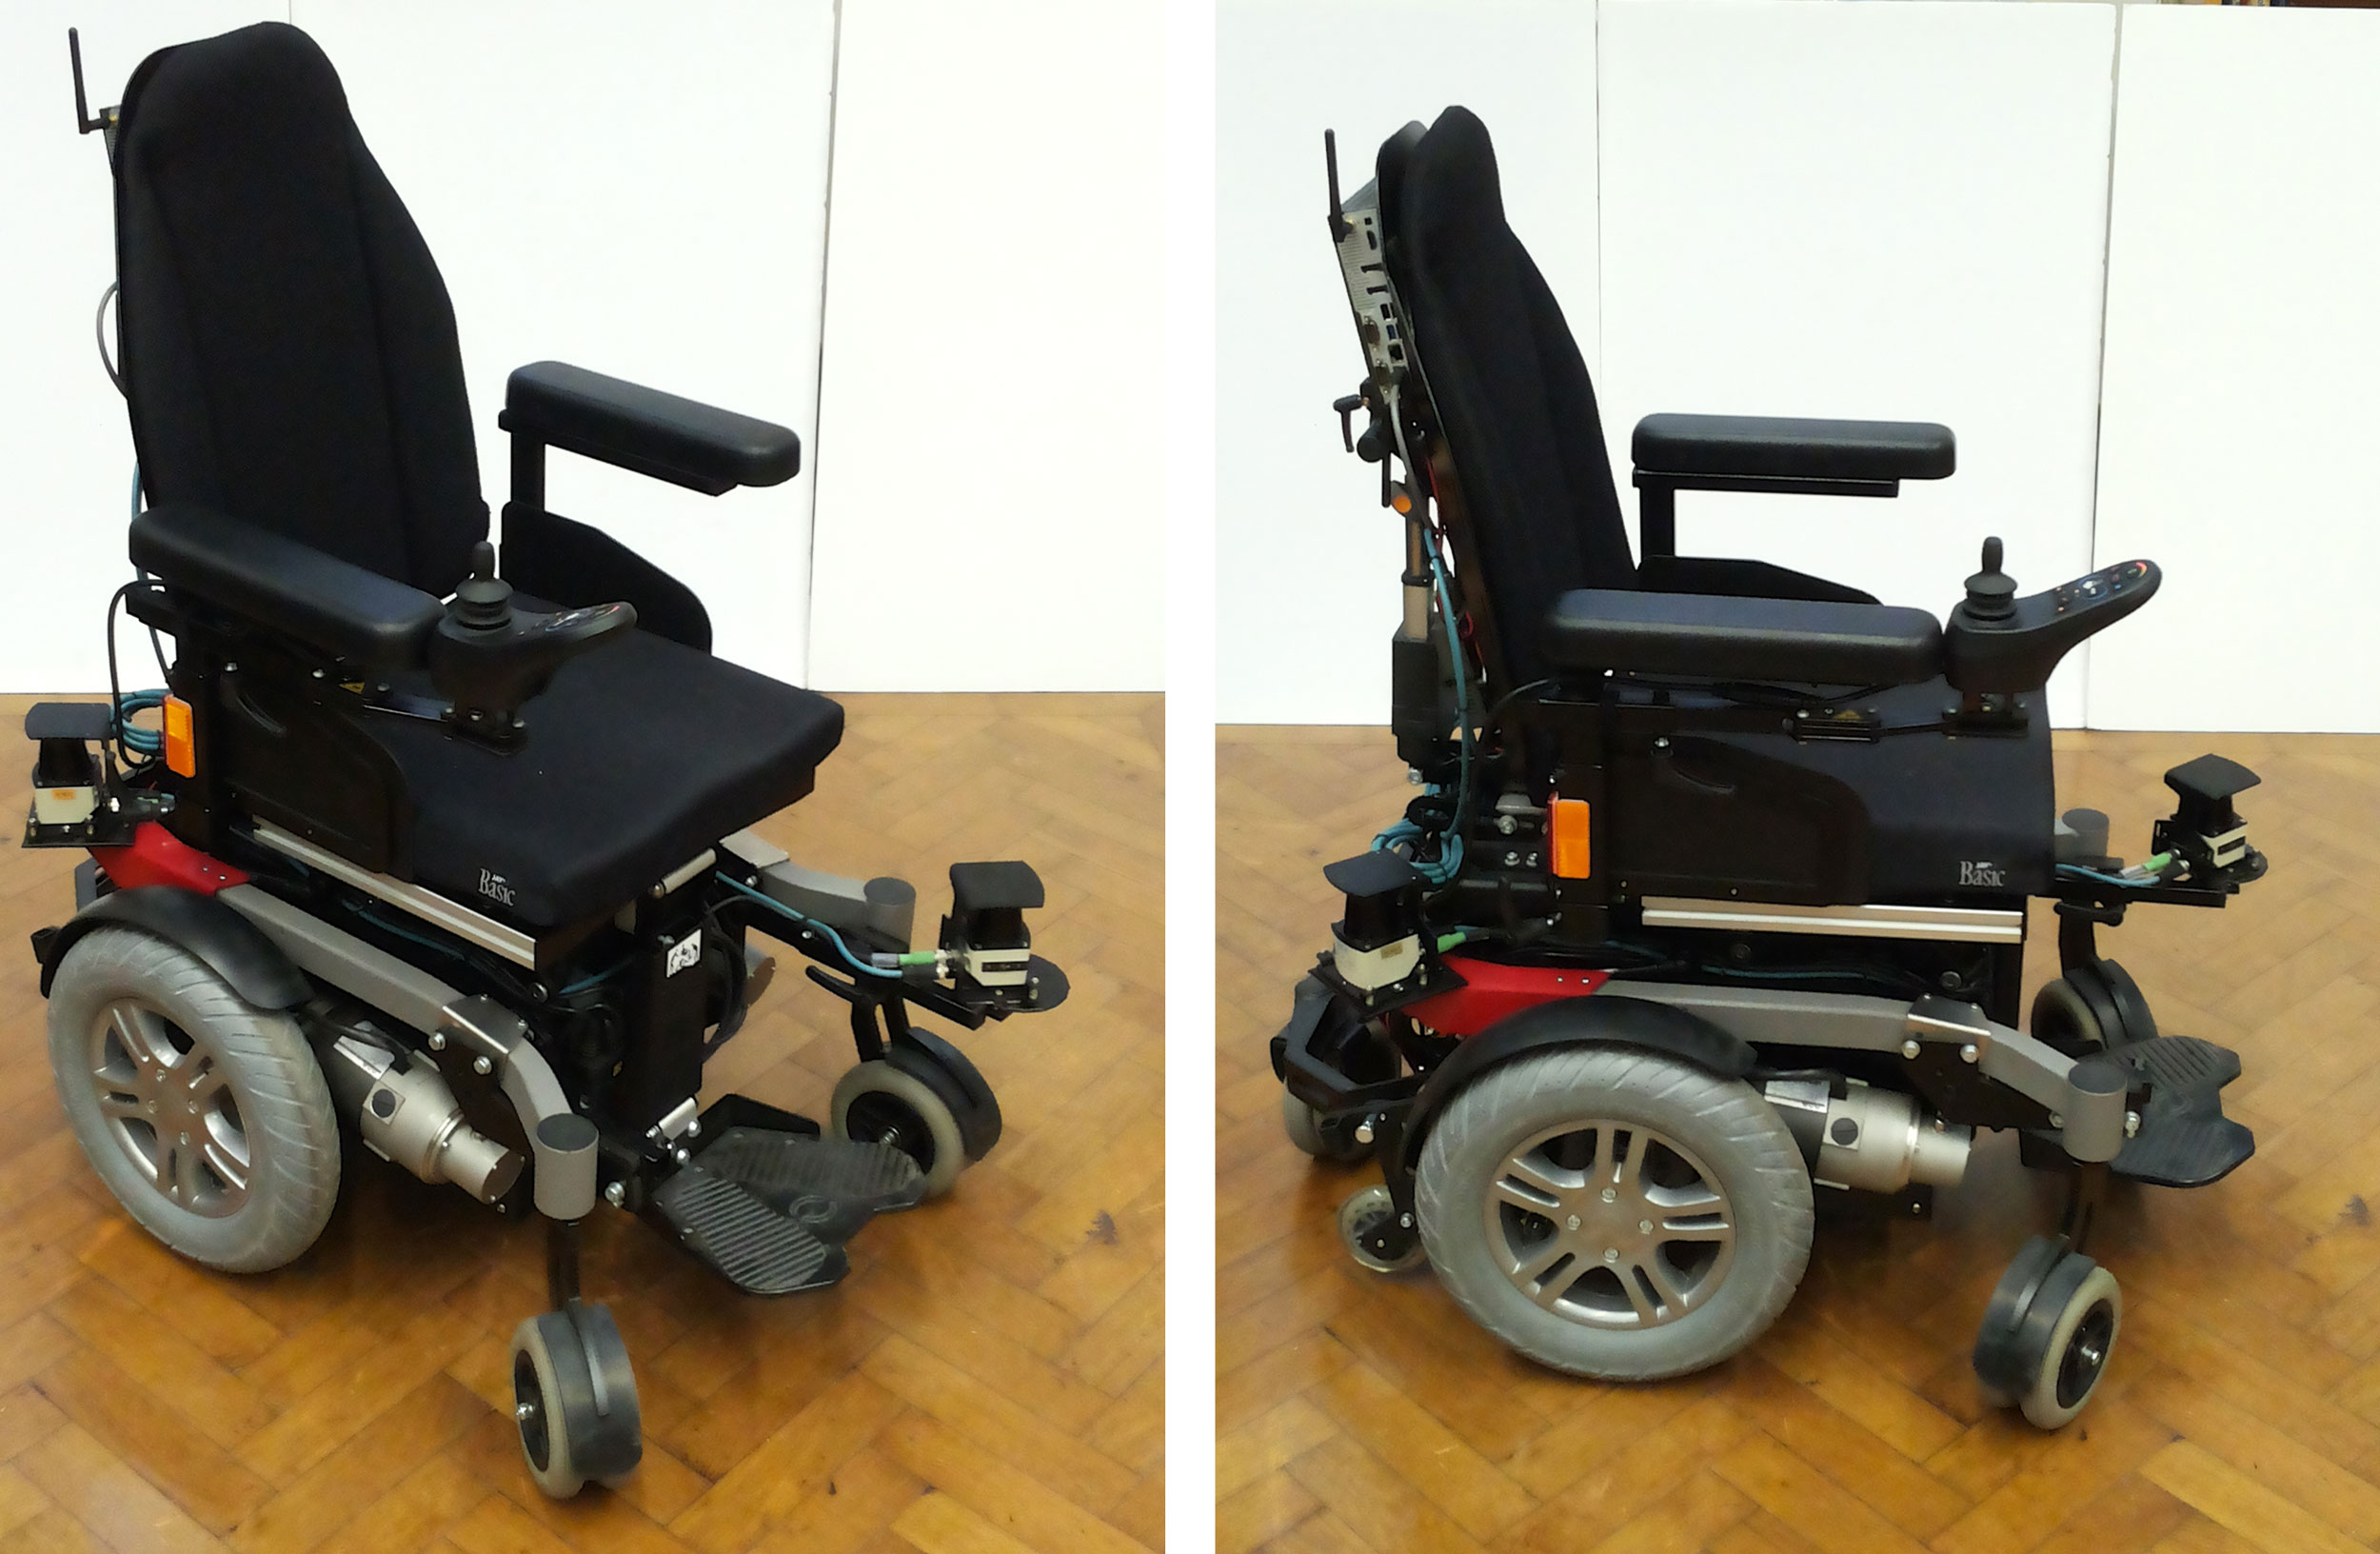
\includegraphics[width=0.95\textwidth]{gfx/pmk/pmk_plat}
\caption{TODO}
\label{fig:pmk}
\end{figure}


\section{The PMK use case}
\label{sec:pmk}
In this section we give a detailed description of a test use case where a model-based approach has been used to replicate and reimplement an existing architecture developed with traditional techniques. We decided to start from an already implemented and fully functional system, to show that is possible to achieve the same level of functionalities of the original application with a model-based design combined with automatic programming.

The target robot is an electric wheelchair modified to be controlled with a computer, and equipped with various sensors to achieve levels of autonomy and teleoperation. The wheelchair used as the starting platform is a commercial model (\textit{Twist T4 2x2}) produced by Degonda Rehab SA; it is suitable for both indoor and outdoor usage and it has high manoeuvrability thanks to the two-wheeled dynamics. The conversion from traditional electric wheelchair to autonomous robotic platform is achieved using the Personal Mobility Kit (PMK), which consists in four elements.
\begin{itemize}
\item Encoders connected to the electric motors controlling the wheels, they provide odometry information.
\item Two \textit{Sick TiM 561} laser scanner distance sensors, they provide a 360-degrees coverage around the wheelchair. They are used to map the environment, assist in the localisation of the robot and detect unexpected obstacles.
\item \textit{Shuttle DS81L}, an high-performance slim PC specifically designed for automotive and robotics applications. It is the on-board computer of the robot, it runs ROS and all the application code.
\item The software components necessary to achieve the assisted and autonomous functionalities.
\end{itemize}
The PMK is designed to be an add-on that is possible to mount over any existing electric wheelchair to convert it into an autonomous or semi-autonomous platform. Thus, of the architecture we will present, the only platform specific part is the interface used to interface with on-board electronics, everything else is a modular design that can be adapted to multiple physical platforms.

A commercial electric wheelchair supports manual control through a joystick placed on one of the armrest. While this is suitable for most of users, there are cases of severe disabilities where the patients can only partially or cannot operate the joystick. The objective of PMK is to extend the functionalities of an electric wheelchair to provide assisted and autonomous control. In particular, the implemented software supports four different drive modes.

\paragraph{Manual with PMK off} This is the native configuration of the wheelchair, the user controls the movements directly with the on-board joystick. It is important to maintain the original operational mode even after the modification introduced by the PMK, the electric wheelchair should remain completely functional and operative even if an hardware or software malfunction causes the PMK to stop working. This act as a fallback emergency configuration.
\paragraph{Manual with PMK on} In this configuration the PMK is active, but the user is still completely in control of the wheelchair. When mediated by the software system, the robotic platform can be controlled remotely by using a wireless joypad or directly with the on-board joystick, a priority system ensures that the input from the joystick always has precedence over teleoperation. This is the neutral configuration of PMK, when the system is active, but not performing any action. This mode is particularly useful during the set up phases of the autonomous wheelchair (\eg, environment mapping).
\paragraph{Assisted} In this mode the PMK is enabled and actively meditates the commands coming from any input device. The aim of this configuration is to help the user operate the wheelchair by avoiding obstacles. Set-points sent from the wireless joypad or on-board joystick are processed and, if necessary, modified to avoid obstacle perceived by the two on-board laser scanners. As for the previous mode, the commands coming from the joystick have the priority over the wireless joypad.
\paragraph{Autonomous} Here the wheelchair is fully autonomous, the PMK is in charge of controlling the movements. The user can request a specific goal (\eg, ``take me to the kitchen''), then the robotic platform will automatically reach the destination avoiding any obstacle along the way. For safety reasons, it is always possible to override the commands sent by the PMK in autonomous mode using the on-board joystick.

\medskip
These are all the main functionalities of the electric wheelchair when equipped with the Personal Mobility Kit. Our aim is to create a system designed and developed using a model-based approach combined with automatic programming that exploits all the problem-related implementations already created for the original architecture and combine them with automatically generated ROS nodes, while maintaining the same functionalities.

\begin{landscape}
	\begin{figure}[t]
	\centering
	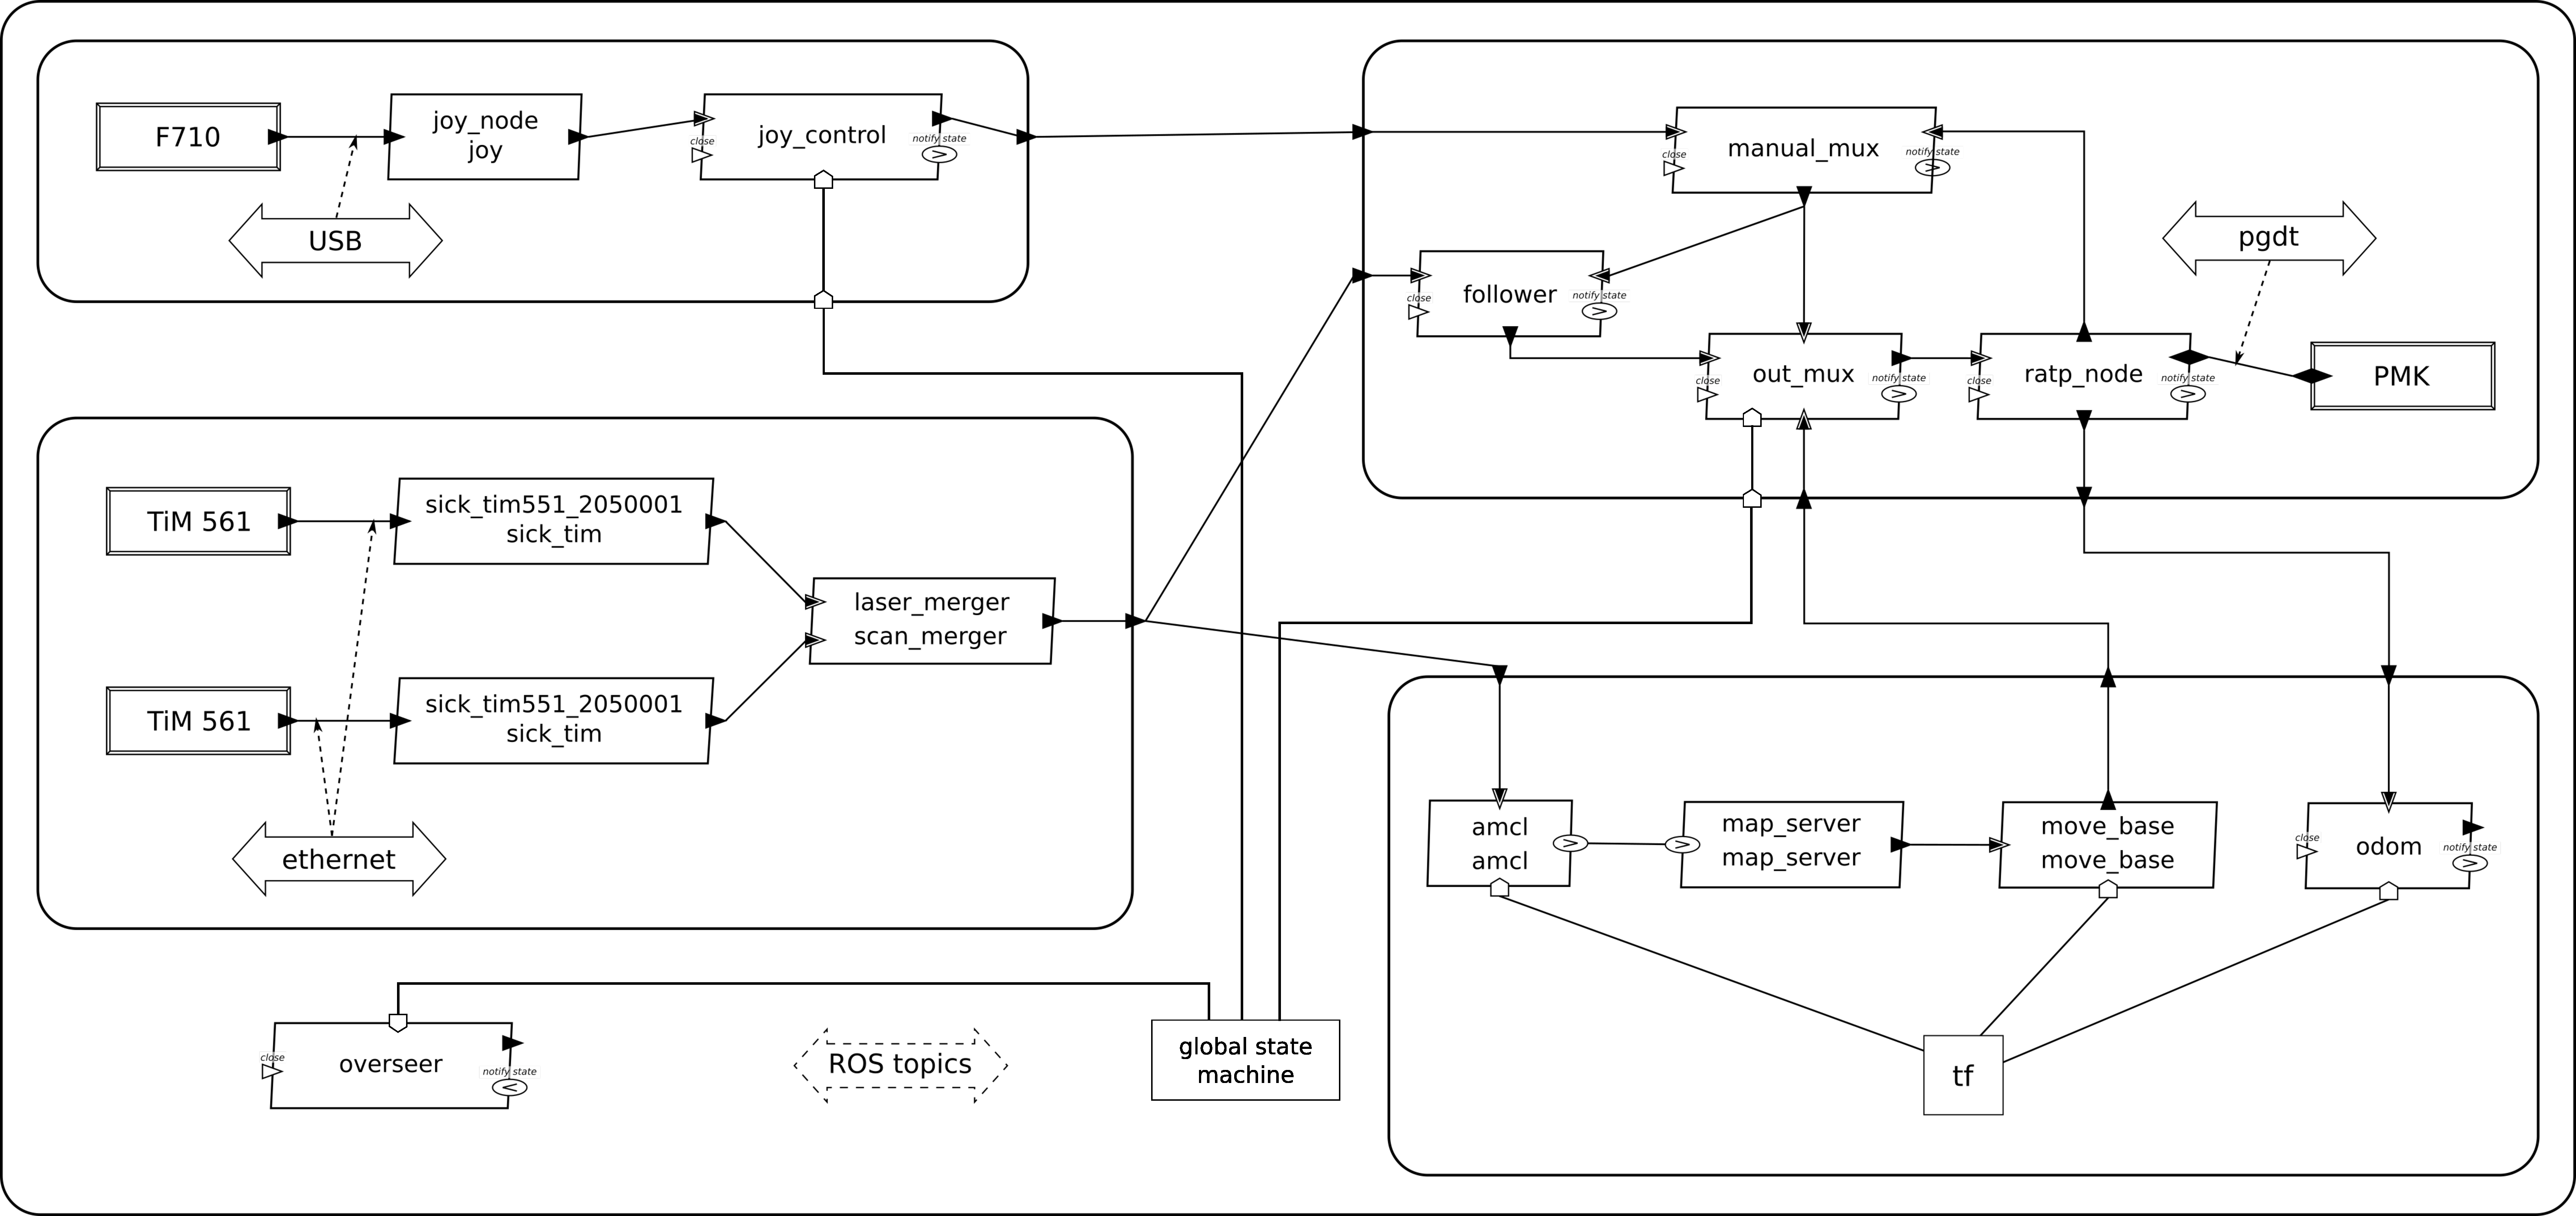
\includegraphics[width=0.95\textheight]{gfx/pmk/model}
	\caption{TODO}
	\label{fig:pmk-model}
	\end{figure}
\end{landscape}


\subsection{Model}
\label{sec:pmk-model}
The first step of the design of an architecture is to create the model. We did so by following the definitions and meta-models introduced in Chapter~\ref{ch:Modelling}. Figure~\ref{fig:pmk-model} shows a graphical representation of the complete model of the architecture of the robotic wheelchair. To organise and generalise the architecture we exploited the nesting capability of AADL by creating a hierarchical structure of system of systems. Each subsystem capture a specific functionality of the robot, and they are meant to be modular parts of the design that can be replaced when necessary. For example, going from laser scanner to cameras, or replacing the navigation system based on \textit{move\_base} with a custom one, or using a different electric wheelchair as platform.

\paragraph{Teleoperation} Similarly to the example presented in Section~\ref{sec:ros-arch}, this subsystem captures all the hardware and software components necessary to implement teleoperation. This specific models includes an AADL device modelling the wireless joypad used to control the wheelchair, a Logitech Gamepad F710. Directly connected to it, the device driver, the existing ROS node \textit{joy\_node} from the package \textit{joy}; it reads the input from the joypad and converts it to ROS messages. The connection between the device and the driver is bound to an AADL bus modelling the physical USB interface between the joypad and the computer. The last software component in the subsystem is a node specifically designed for this application, \textit{joy\_control} is in charge of converting the messages coming from the device driver to velocity set-points to directly control the wheelchair (\ie, from \textit{Joy} to \textit{Twist} messages). Additionally, this node controls the global state machine of the system that selects the current driving mode (\ie, one of the four presented in Section~\ref{sec:pmk}), given the criticality of this communication it does not happen through ROS topics or services, but by accessing directly a shared memory area. This behaviour is captured in the model using a require data access port on the process modelling \textit{joy\_control}. On its frontier, the system exposes an outgoing port associated with the velocity command to relay the set-points generated by the teleoperation subsystem to the rest of the architecture; moreover it has a data access to bridge the connection coming from the driving mode selection node (\ie, \textit{joy\_control}) to the shared memory area hosting the global state machine. Encapsulating the model in a system increases the modularity of the design, since it defines exactly the expected interfaces of the subsystem and makes it replaceable with a similar configuration (\eg, a different physical input) without altering the entire architecture.

\paragraph{Sensing} For the navigation and obstacle avoidance to work correctly, they need a single measurement from the laser rangefinder. Since the robotic platform is equipped with two sensors, the aim of the sensing subsystem is to unify their measurements in a single output; for this reason only one outgoing port is present on the system frontier representing the merged scan topic. Here there is a clear example on how multiple instances of same element can coexist as subcomponents. There are two occurrences of the same AADL device modelling the physical sensors mounted on the wheelchair, consequentially, the device driver component is duplicated too. As for the teleoperation subsystem, the connection between each laser scanner and the corresponding driver is bound to a model of a physical bus; but since the communication goes through an Ethernet connection it is a different component. All the connections converge in a single node in charge of merging the measurements coming from each laser rangefinder, that are then relayed outside the subsystem through the output port present on the frontier. In this system there is no custom node, since all of them come from existing packages or legacy implementations.

\paragraph{Navigation} This subsystem mostly contains legacy nodes from ROS Navigation. A node implementing adaptive Monte Carlo localisation to estimate the position of the robot in a known environment (\textit{amcl}), a node to store and share the current map of the environment (\textit{map\_server}), and the main navigation node (\textit{move\_base}) implementing global planning on the known map and local planning on the map generated in real time. To work, ROS Navigation requires laser measurements and odometry information, the former comes from the sensing subsystem, while the latter is generated by the custom \textit{odom} node included in the navigation subsystem; it receives the current speed from the wheelchair and uses it to estimate the position of the platform. The odometry node supports two types of output, as visible from the features of the AADL process, an \textit{Odometry} message, published on a topic and modelled using an output port, and shared using \textit{tf}, modelled thorough a data access directly connected to the data component representing the centralised collection of all the reference frames. Since it is the backbone of ROS Navigation, and it is used only by nodes in this subsystem, it was reasonable to model the data component representing \textit{tf} here. Differently from the two previous subsystems (\ie, teleoperation and sensing), here there is no need to model any physical bus since this is a pure software system. The frontier of the navigation subsystem is more complex, since it has an input port for the laser measurements, another input port for the speed of the wheelchair and  an output port for the set-point generated by \textit{move\_base}. Abstracting the structure and interface of the navigation subsystem is particularly important since it is the part of the architecture that is more subject to changes, it is common to use the same platform to test different algorithms and architectural solutions for navigation.

\paragraph{Platform} All the hardware and software components related to the physical platform are contained in this subsystem, since they are all platform-related, each node is a custom design created specifically for this architecture. There are two hardware components: a device to model the interface between the architecture and the on-board electronics manufactured by Penny\&Giles Drive Technologies Ltd. (PGDT), and the bus representing the special hardware connection used to exchange wheelchair-specific messages. This bus and the corresponding custom device driver (\textit{ratp\_node}) act as a bridge between platform-specific data streams and ROS messages. Given the multiple driving modes of the robot where two manual inputs, potentially mediated by the system and with different priorities, coexists, together with an autonomous mode, the architecture uses a combination of two multiplexers. One is used to select the specific manual input (\ie, \textit{manual\_mux}), while the other (\ie, \textit{out\_mux}) differentiate between the different driving modes (\ie, manual, assisted and autonomous). The two multiplexers have different behaviours, \textit{manual\_mux} is based on priorities, the input coming from the the on-board joystick will always override the wireless joypad, while \textit{out\_mux} changes the output depending on the current mode of the system, for this reason this component has a data access connected to the shared memory area hosting the global state machine. Finally, the last component is a node implementing local obstacle avoidance for assisted driving. Even with its peculiar configuration, the whole subsystem is designed with a general frontier, it exposes two inbound ports for the velocity commands (\ie, joypad and autonomous set-points) and one for scan messages (\ie, measurements for obstacle avoidance). The output port relays the current velocity of the wheelchair from the custom device driver node to the navigation subsystem. Additionally, as for the teleoperation subsystem, the platform system has a data access on its frontier to connect to the global state machine. By encapsulating the platform in a system, it is possible to replace it with a different wheelchair, or even with a completely different robotic platform.

\begin{figure}[t]
\centering
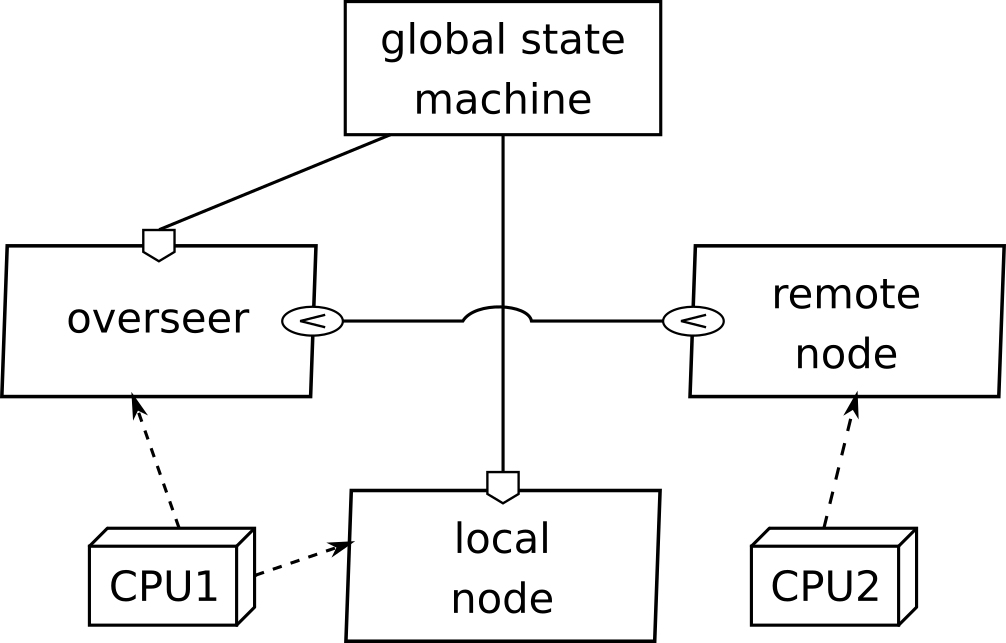
\includegraphics[width=0.7\textwidth]{gfx/pmk/overseer}
\caption{TODO}
\label{fig:pmk-gsm}
\end{figure}

\paragraph{Main system} To increase clarity and use the model to evoke the modularity of the architecture, we modelled it with different subsystems. However, in AADL it is necessary to define a root system to encapsulate everything, moreover, some part of the architecture are too general to be fitted in a specific subsystem. For this architecture, three components fall in this category: the \textit{ROS communication} virtual bus, the \textit{overseer} node and the global state machine. In the same way as physical buses are used in the teleoperation and platform subsystems, the \textit{ROS communication} virtual bus is necessary to identify which connections model ROS communication protocols (\ie, topics or services), this is done by binding them to it. As originally introduced in Section~\ref{sec:ros-in-aadl} and, later, detailed in Section~\ref{sec:ros-node}, the engineered nodes are designed with a strict life cycle, and they natively support a notification system to monitor the evolution of their state. The \textit{overseer} node is in charge of collecting all the notification coming from the custom nodes, moreover it has a list of all the critical nodes (\ie, nodes that are subject to a liveness check) and trigger a transition on the global state machine if one of them stops working. The last element is the data component representing the shared memory area containing the global state machine. In the implementation, the global state machine is instantiated by the \textit{overseer}, while all the nodes in the architecture can read or modify the current state by accessing the shared memory directly, it is also possible to interact with the global state machine through a ROS service interface mediated by the \textit{overseer} (see Figure~\ref{fig:pmk-gsm}). The different approach used can be encoded in the model (\ie, connected through a data access or a subprogram call) however, in the implementation, it is determined at deployment time. In practice if the node runs on the same physical machine of the global state machine, then a shared memory approach is used, otherwise the interaction happens using ROS. 

\subsection{Automatic code generation}
In the previous section, we gave an overview of the model of the architecture by describing in details the subsystems and which functionalities they evoke. While the graphical representation of Figure~\ref{fig:pmk-model} provides a general understanding of the topology of the architecture and gives some insights on the nature of the components, it does not capture all the details necessary to correctly perform automatic code generation. First of all, nodes belongs to three main categories: already implemented nodes, they are legacy nodes previously developed, they may come from the standard ROS repositories (\eg, \textit{move\_base}) or be part of the original architecture (\eg, \textit{laser\_merger}), custom nodes, they are completely modelled and will be automatically generated (\eg, \textit{odom}), special custom nodes, they are modelled correctly, but they contain unique implementation patterns that are not supported by the code generator (\eg, \textit{ratp\_node}). This last category will be covered in details in Section~\ref{sec:special-node}. 

As discussed in Section~\ref{sec:ros-arch}, managing existing nodes in the architecture model is extremely important, since they are an invaluable resource provided by the ROS community. During the automatic code generation, existing nodes are ignored, since they do not provide any internal implementation but are described only as interfaces, however, they are correctly included in the generation of launch files describing the current configuration of the system. Moreover, connections between components can be specialised using properties to exploit topic remapping and define the runtime name of each topic, included those of already implemented nodes. Currently, the code generator does not support the use of neither ASN.1 nor JSON schema to define the parameters of the legacy nodes, however,  it is possible to use properties to specify a standard ROS YAML file to be automatically included in the launch file as the parameter configuration of a specific node.

To automatically generate custom nodes that are compilation-ready, it is necessary to specify a series of properties. On a basic level, the designer can tune the behaviour of publisher and subscriber by setting the frequency, the queue size or the default name of the topic. Moving to a domain-specific point of view, the developer has to provide the implementations of the nodes; for this reason we decided to base our test use case on an existing architecture to exploit already implemented problem-specific code for the automatic programming phase. To understand how the process works in practice, let us take the example of the \textit{follower} node. Without consider the domain-specific implementation, this component evokes a combination of a \textit{sink} behaviour, the subscriber receiving the messages from the laser rangefinder, and a \textit{filter} behaviour, manual set-points are received, modified according to the scan measurements, eventually modified and published. This configuration is translated to the code generator to two subscribers (\ie, one for the laser and one for the input commands) and a publisher (\ie, the output set-point). Moreover, by parsing the JSON files specified as properties in the component definition, the code generator can create the internal state of the node and set default and initial values for parameters and variables. After generating all the necessary source files, it is possible to include the domain-specific implementation as an external library, defined again in properties of threads and subprograms; this is done by carefully generating all the build files that bind together the auto-generated node skeleton and the manually implemented problem-specific code. When all the file related to the node are fully generated (\ie, core node implementation, internal state, external libraries, and build configurations), it is time to create the launch files. Since the \textit{follower} node is part of the platform subsystem, it will be included in the platform-specific launch file, here the runtime configuration of the node is generated from the JSON files and included, moreover, as for the legacy nodes, the topics name are remapped according to the properties defined on the connections in the model. At this point, the generation of the node is complete and it is ready to be compiled and run.

\begin{figure}[t]
\centering
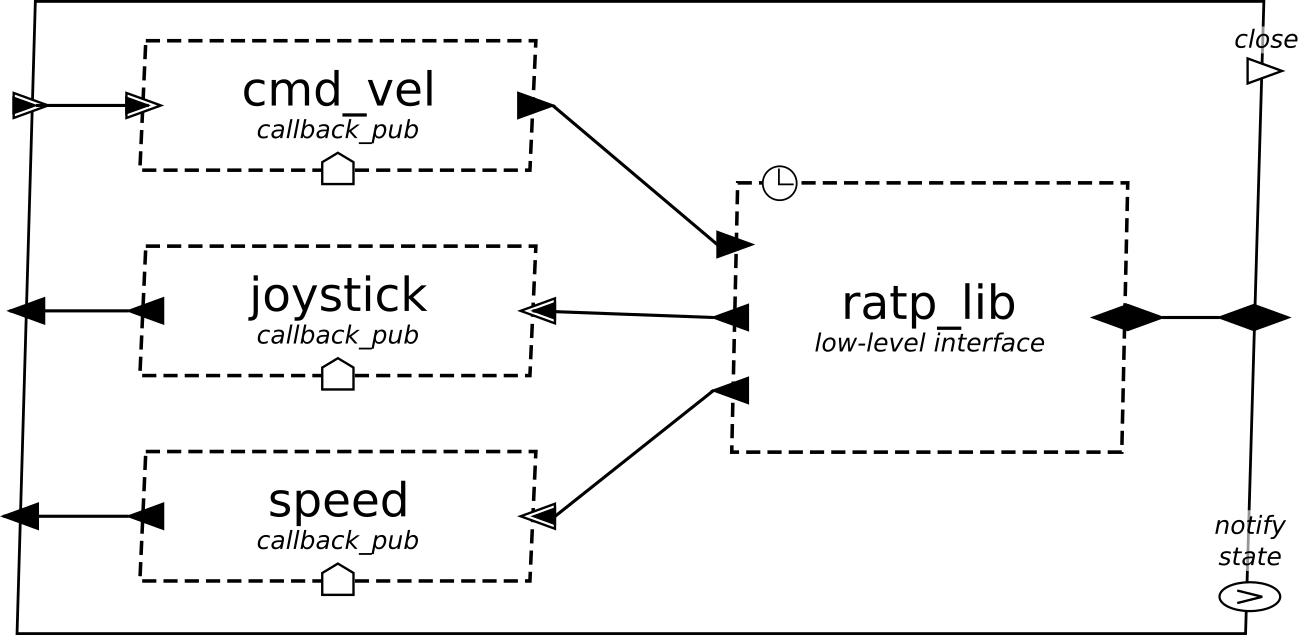
\includegraphics[width=0.95\textwidth]{gfx/pmk/ratp}
\caption{TODO}
\label{fig:pmk-ratp}
\end{figure}

\subsection{Special nodes}
\label{sec:special-node}
Since all the problem-specific logic was already implemented in the original architecture, every element of the new system is generated using the automatic programming approach. There is only one exception: the \textit{ratp\_node}; this node is the device driver connecting the low-level electronics of the wheelchair to the ROS-based architecture. It implements a unique interface between ROS messages and custom data streams defined by the PGDT bus, therefore it is very challenging to automatically generate the source code using an automatic programming approach. Since this node is an hybrid between a ROS-based (\ie, receiving set-points and publishing the current speed and status) and an hardware-specific (\ie, interfacing with the PMK) implementation, we can partially exploit the code generator to define a node skeleton to be refined by the developer. There are two key challenges when using this approach: first, to have a model expressive enough to capture the peculiar design of the component, and second, to generate a node in such a way that the hardware-specific functionalities can be integrated without major modifications.

To tackle the first challenge we can exploit the expressive power provided by AADL. When not extending our base templates (see Section~\ref{sec:template}) used to identify ROS elements,  AADL connections, ports and threads can be used to model any kind of communication protocol or execution flow. Figure~\ref{fig:pmk-ratp} shows a simplified (recurring elements of the base ROS node are omitted) graphical representation of the model of the \textit{ratp\_node}. It is possible to use a periodic AADL thread together with a bidirectional port on its frontier to model the communication between the component and the low-level hardware. Additional ports model the exchange from a problem-specific implementation to the ROS communication protocols.  The \textit{ratp\_lib} thread produces two outputs that are converted to ROS messages: one is the current set-point provided by the on-board joystick, and the other is the current speed of the wheelchair. Moreover, it receives one input from the rest of the system that is then converted to a format compatible with the low-level hardware: the set-point of the current active input. These port on the frontier of the low-level communication thread are connected using internal connections to the corresponding threads modelling the publishers and subscribers. However, there is a significant distinction between this model and how ROS thread are usually modelled. Threads behaving as subscribers are not triggered by a message coming from outside the component, but directly by the \textit{ratp\_lib} thread, moreover, the publisher thread output does not relay its message to the rest of the architecture, but the output port is connected directly to the low-level communication thread.

The second challenge is implicitly solved by the design of the engineered node and how unknown subcomponents are managed by the code generator.  As explained in Section~\ref{sec:xml-cpp}, the code generator parses a process model and implements it as a ROS node, only if it extends the base ROS node model, moreover, of all the threads defined as subcomponents those that do not extend one of the predefined functionalities (\ie, publisher, subscriber, subscriber with publisher or service) are ignored and not processed by the automatic programming system. In the case of the \textit{ratp\_node} it means that the code generator recognises the component as a ROS node and generates all the basic structure, additionally, the three thread modelled as ROS elements (\ie, \textit{cmd\_vel}, \textit{joystick} and \textit{speed}) but connected to the \textit{ratp\_lib} thread are correctly generated as ROS subscribers or publishers. In summary, given the model presented in Figure~\ref{fig:pmk-ratp}, the resulting generated node extends the engineered node and correctly implements the life cycle, the asynchronous spinner, the encapsulated internal state and the separation between the middleware and the problem-specific code; moreover it contains three publishers and three subscribers. Out of these six ROS functionalities, three are already correctly implemented: the publisher for the current speed and the current command of the on-board joystick, and the subscriber for the external set-point. The other three needs to be converted from a ROS-based design to an implementation compatible with the low-level interface. While this approach may appear as an over-complication, it actually streamlines the work of the developer. The code generator handle automatically all the ROS-related boilerplate, while defining a structure that can be easily exploited; the developer only needs to focus on implementing the thread interfacing with the low-level hardware. In our implementation, we use the already created structure as a reference and replaced the callback structure of ROS with standard bindings. Basically, from the point of view of the node, the interaction still happens through a system of callbacks, however, they are not triggered by ROS, but controlled by the \textit{ratp\_thread}. 

In conclusion, while this node requires a direct intervention of the developer to modify its structure, it is more efficient to model it, generate the code to obtain a partially implemented component and then manually insert some modifications, instead of implementing it from scratch. This is possible because of the modularity and flexibility of the engineered node, and because ROS is still the main element of the component design. While our code generator currently cannot completely and successfully process this type of nodes, this mixed approach (\ie, code generation combined with heavy human intervention) gives us an insight on how future nodes with the same characteristics could be automatically generated.


\begin{landscape}
	\begin{figure}[t]
	\centering
	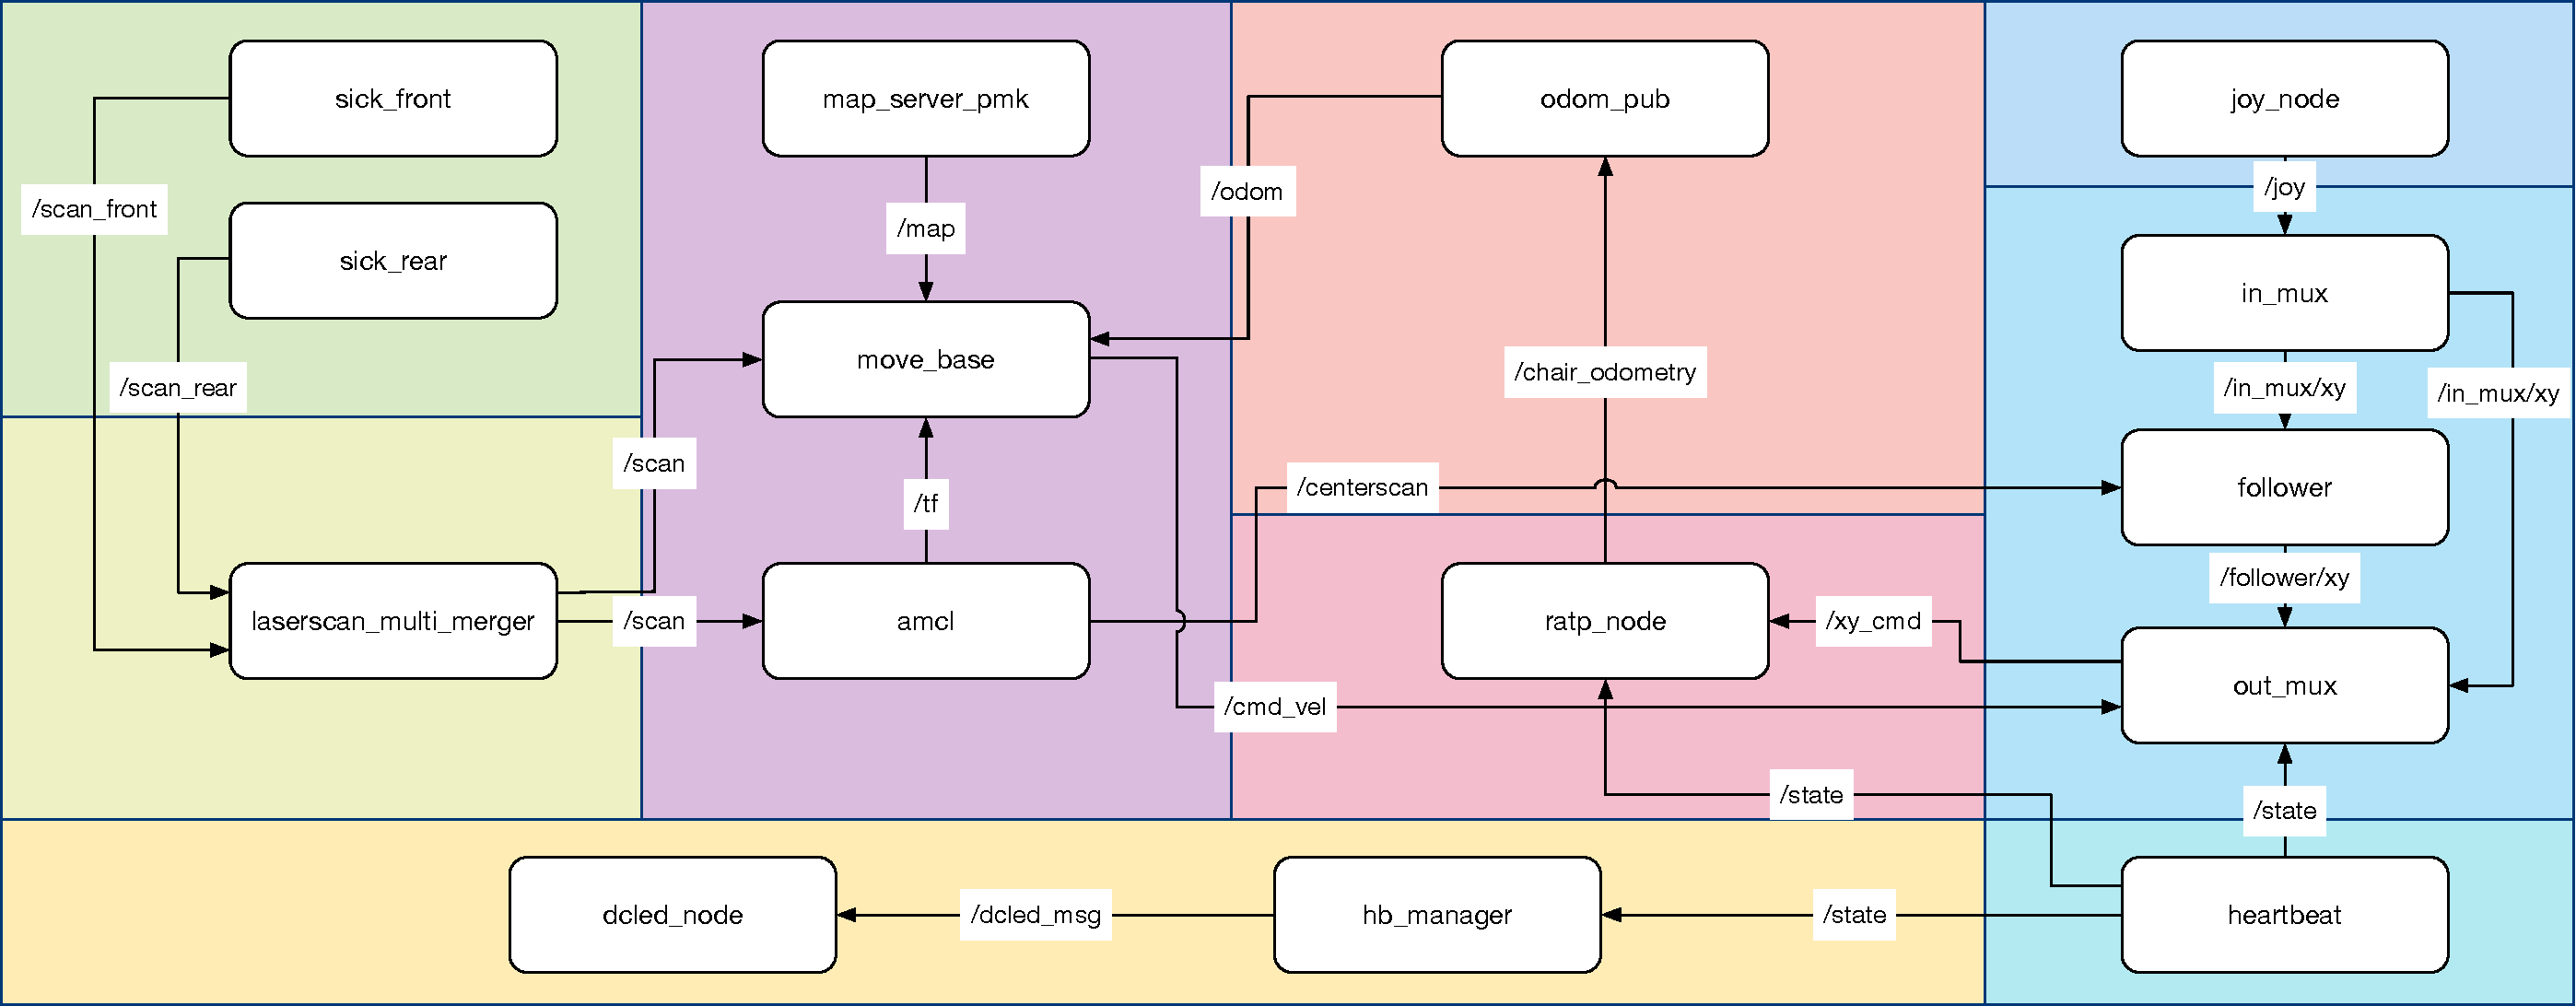
\includegraphics[width=0.95\textheight]{gfx/pmk/softwarearchitecture}
	\caption{TODO}
	\label{fig:pmk-doc}
	\end{figure}
\end{landscape}

\begin{landscape}
	\begin{figure}[t]
	\centering
	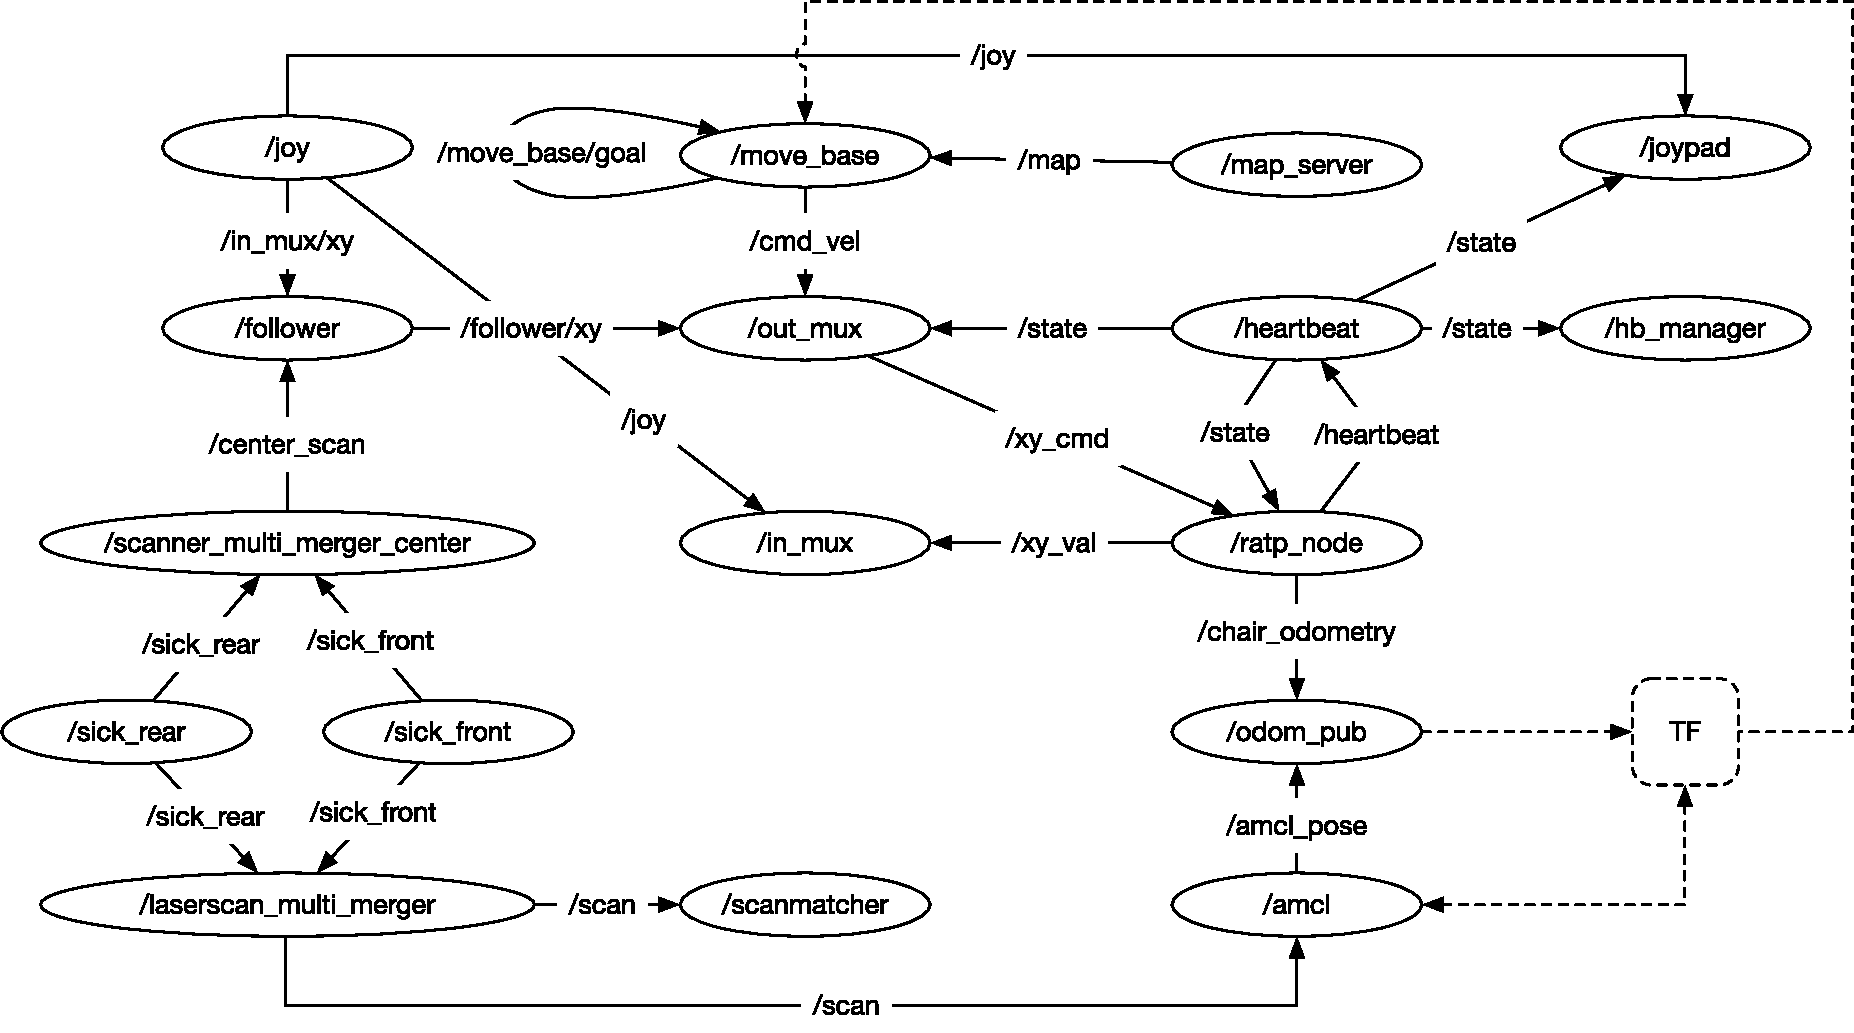
\includegraphics[width=0.95\textheight]{gfx/pmk/hand-graph}
	\caption{TODO}
	\label{fig:pmk-graph}
	\end{figure}
\end{landscape}

\begin{landscape}
	\begin{figure}[t]
	\centering
	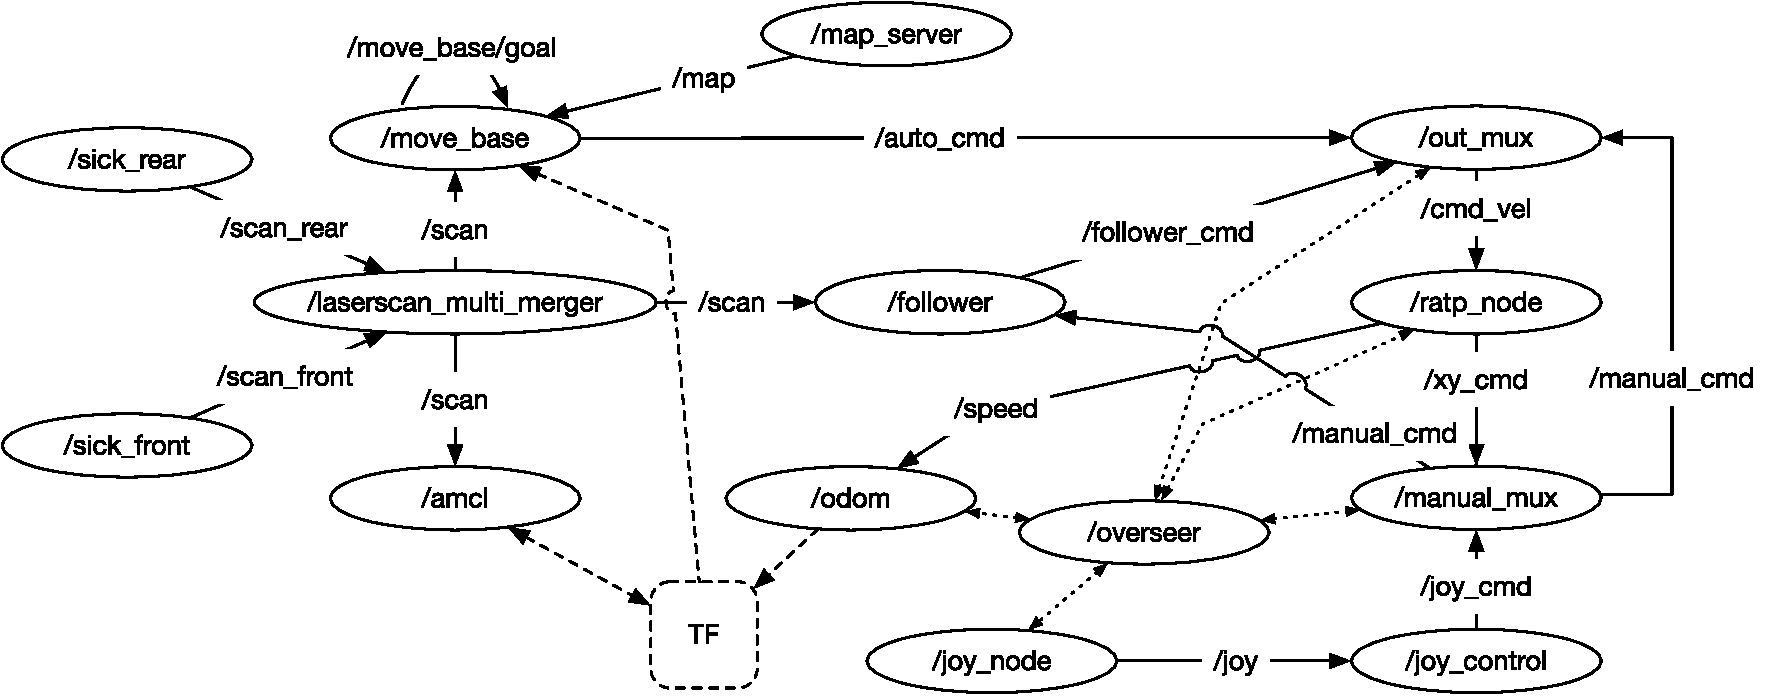
\includegraphics[width=0.95\textheight]{gfx/pmk/gen-graph}
	\caption{TODO}
	\label{fig:gen-graph}
	\end{figure}
\end{landscape}

\begin{figure}[t]
\centering
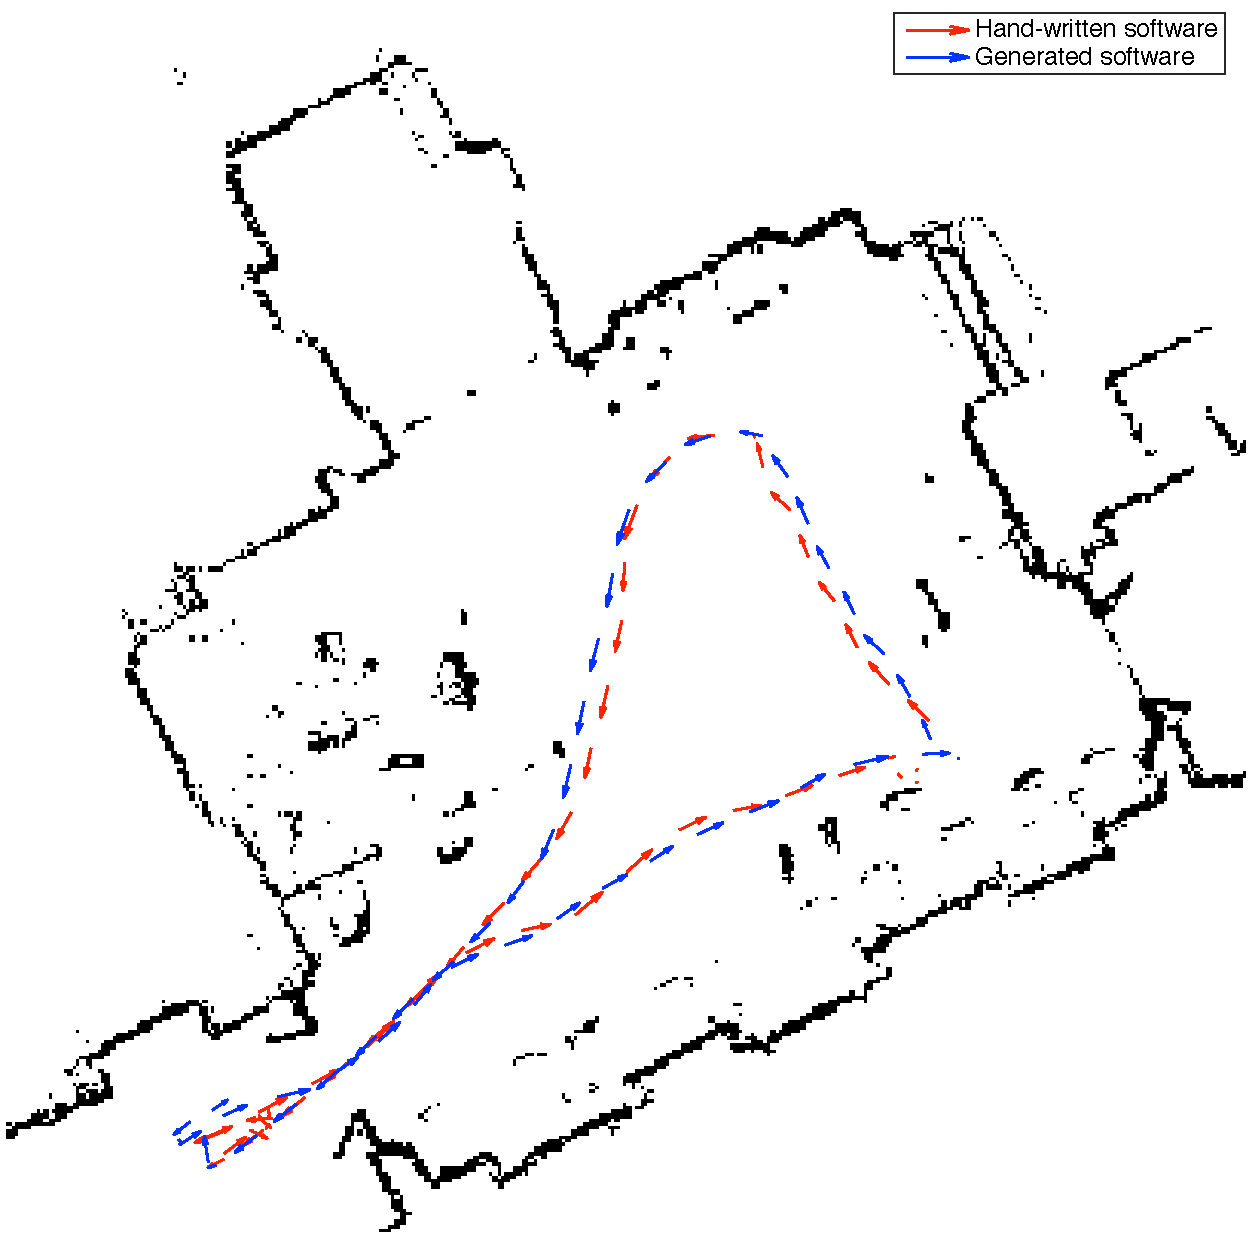
\includegraphics[width=0.95\textwidth]{gfx/pmk/path-followed}
\caption{TODO}
\label{fig:path}
\end{figure}

\subsection{Comparison}
The aim of this use case was to showcase how a complete and functional architecture can be designed and developed entirely using a model-based approach combined with automatic code generation. Starting from an existing architecture was useful for multiple reasons: clear use case and requirements for the robot, existing implementations for all the problem-specific features, precise target functionalities, reference benchmark for the behaviour of the autonomous wheelchair. It was important for us to be able to compare the result of our approach to an existing implementation. In this section, we will analyse the original architecture to show the parallels with the automatic generated one and to highlight existing problems that were solved using a model-based design approach.

First of all, we have to compare the design of the architecture of the wheelchair according to the documentation (Figure~\ref{fig:pmk-doc}) with the runtime computation graph generated by ROS (Figure~\ref{fig:pmk-graph}). With a quick analysis it is possible to see that they do not match, some nodes mentioned in the documentation are not present in the graph (\eg, \textit{dcled\_node}) or vice versa (\eg, \textit{scanner\_multi\_merger\_center}), while others have been replaced (\eg, the standard \textit{map\_server} in place of the custom \textit{map\_server\_pmk}). This is not surprising, the PMK is an ongoing research project where multiple people with varying experience contributed to it. As a result, features were added directly to the codebase without propagating them in the documentation or in the original design. As the project progressed, some of the features were removed, but they left some dangling dependencies behind, in the form of design choices and components. This problem is exacerbated by the fact that ROS does not provide any tool to visualise and analyse the complete architecture before runtime, the only way is to run the entire system and then view the computational graph using tools like \textit{rqt\_graph}. However, even this approach is limited, since it only shows topics, but no services or actions. Of course, a model-based approach does not automatically solve all these problems, since a developer can, and sometimes needs to, directly modify the codebase; however, by combining models and automatic code generation we can create an environment where good practices and designs are encouraged and more natural.

With a deeper analysis of the computational graph it is possible to identify some architectural problems, that were not present in the original design but were introduced in sequential iterations of the project. There are three fundamental issues that could cause unexpected behaviours of the robot.
\begin{itemize}
\item There is a circular dependency between \textit{odom\_pub} and \textit{amcl}. Both nodes are in charge of estimating the position of the robot, the former uses velocity measurement coming from the wheelchair, while the latter matches laser rangefinder data with a know map. The circular dependency happens because each of them expect from the other an initial position to start the estimate. Given how the two algorithms are implemented, an incorrect starting position would not compromise the correct functioning of the system, however it may cause unexpected behaviour, especially after the initial start up of the system.
\item The odometry is estimated twice in the system. This is not directly visible from the graph presented in Figure~\ref{fig:pmk-graph}, since it is not detailed enough, however, the \textit{rapt\_node} pre-compute the odometry of the platform and provide it, together with the velocity measurements, to \textit{odom\_pub}. The initial computation is then discarded and recalculated again directly from the velocity. While this causes no malfunction, it is not a consistent design choice to do a specific processing twice in the same architecture. 
\item The management of the laser scanner measurements is flawed in multiple ways. As explained in Section~\ref{sec:pmk-model}, the navigation subsystem requires an unified source of laser information. In the original documentation, there was a single node in charge of merging the two laser sources, however, in the actual architecture, there are two nodes with the same task: \textit{scanner\_multi\_merger\_center} and \textit{laserscan\_multi\_merger}. Moreover, it is not visible from the computation graph, but the lunch file of the original architecture included a third laser scan merger node,  which it is killed at start up since it has the exact same name of another one, and ROS forbid it. Finally, there is a \textit{scanmatcher} node that subscribe to a topic but has no role in the architecture, a leftover dependency from a removed functionality. Since the duplicated nodes are functionally identical, the overall functionality of the architecture are preserved. However, such a configuration is a waste of computational power and a potential source of significant and dangerous inconsistencies.
\end{itemize}

For comparison, Figure~\ref{fig:gen-graph} shows the computational graph of the architecture resulting from the model-based design and automatic code generation. The overall structure of the system is very similar to the original architecture, however, all the issues identified before have been solved.
\begin{itemize}
\item There is no circular dependency between \textit{amcl} and \textit{odom}. They receive the initial position independently as a parameter or through an external topic.
\item The odometry is estimated only once in the \textit{odom} node. The \textit{ratp\_node} provides directly and only the current speed of the wheelchair as a \textit{Twist} message.
\item Only one node is in charge of unifying the laser sources and the \textit{scanmatcher} node has been removed.
\end{itemize}

Analysing the ROS graph it is useful to provide an overview of the quality of the design of the architecture, however, it gives no insight on the actual functionalities of the system. As seen from the original architecture, design flaws not always translate in a compromised system or faulty behaviours. The robotic wheelchair equipped with the handcrafted architecture supported full autonomous driving with no serious issues, except for minor problems caused by an unstable communication with the low-level control module. This means that we can use the behaviour of the original architecture  to provide an empirical proof of the correctness of the generated architecture. We performed a comparison between the path followed by the wheelchair when running the original system in autonomous mode, and then we gave the same goal to the generated architecture; Figure~\ref{fig:path} shows the result. The resulting paths are extremely similar, this shows that not only the generated architecture replicates the same results of the original one, moreover, all the problem-specific implementations have maintained their original functionalities even after they are transposed in the automatically generated ROS environment.

%*****************************************

%\addtocontents{toc}{\protect\clearpage} % <--- just debug stuff, ignore
%%************************************************
\chapter{Math Test Chapter}\label{ch:mathtest} % $\mathbb{ZNR}$
%************************************************
Ei choro aeterno antiopam mea, labitur bonorum pri no. His no decore
nemore graecis. In eos meis nominavi, liber soluta vim cu. Sea commune
suavitate interpretaris eu, vix eu libris efficiantur.

\section{Some Formulas}
Due to the statistical nature of ionisation energy loss, large
fluctuations can occur in the amount of energy deposited by a particle
traversing an absorber element\footnote{Examples taken from Walter
Schmidt's great gallery: \\
\url{http://home.vrweb.de/~was/mathfonts.html}}.  Continuous processes
such as multiple
scattering and energy loss play a relevant role in the longitudinal
and lateral development of electromagnetic and hadronic
showers, and in the case of sampling calorimeters the
measured resolution can be significantly affected by such fluctuations
in their active layers.  The description of ionisation fluctuations is
characterised by the significance parameter $\kappa$, which is
proportional to the ratio of mean energy loss to the maximum allowed
energy transfer in a single collision with an atomic electron:
\graffito{You might get unexpected results using math in chapter or
section heads. Consider the \texttt{pdfspacing} option.}
\begin{equation}
\kappa =\frac{\xi}{E_{\textrm{max}}} %\mathbb{ZNR}
\end{equation}
$E_{\textrm{max}}$ is the maximum transferable energy in a single
collision with an atomic electron.
\[
E_{\textrm{max}} =\frac{2 m_{\textrm{e}} \beta^2\gamma^2 }{1 +
2\gamma m_{\textrm{e}}/m_{\textrm{x}} + \left ( m_{\textrm{e}}
/m_{\textrm{x}}\right)^2}\ ,
\]
where $\gamma = E/m_{\textrm{x}}$, $E$ is energy and
$m_{\textrm{x}}$ the mass of the incident particle,
$\beta^2 = 1 - 1/\gamma^2$ and $m_{\textrm{e}}$ is the electron mass.
$\xi$ comes from the Rutherford scattering cross section
and is defined as:
\begin{eqnarray*} \xi  = \frac{2\pi z^2 e^4 N_{\textrm{Av}} Z \rho
\delta x}{m_{\textrm{e}} \beta^2 c^2 A} =  153.4 \frac{z^2}{\beta^2}
\frac{Z}{A}
  \rho \delta x \quad\textrm{keV},
\end{eqnarray*}
where

\begin{tabular}{ll}
$z$          & charge of the incident particle \\
$N_{\textrm{Av}}$     & Avogadro's number \\
$Z$          & atomic number of the material \\
$A$          & atomic weight of the material \\
$\rho$       & density \\
$ \delta x$  & thickness of the material \\
\end{tabular}

$\kappa$ measures the contribution of the collisions with energy
transfer close to $E_{\textrm{max}}$.  For a given absorber, $\kappa$
tends
towards large values if $\delta x$ is large and/or if $\beta$ is
small.  Likewise, $\kappa$ tends towards zero if $\delta x $ is small
and/or if $\beta$ approaches $1$.

The value of $\kappa$ distinguishes two regimes which occur in the
description of ionisation fluctuations:

\begin{enumerate}
\item A large number of collisions involving the loss of all or most
    of the incident particle energy during the traversal of an absorber.

    As the total energy transfer is composed of a multitude of small
    energy losses, we can apply the central limit theorem and describe
    the fluctuations by a Gaussian distribution.  This case is
    applicable to non-relativistic particles and is described by the
    inequality $\kappa > 10 $ (\ie, when the mean energy loss in the
    absorber is greater than the maximum energy transfer in a single
    collision).

\item Particles traversing thin counters and incident electrons under
    any conditions.

    The relevant inequalities and distributions are $ 0.01 < \kappa < 10
    $,
    Vavilov distribution, and $\kappa < 0.01 $, Landau distribution.
\end{enumerate}


\section{Various Mathematical Examples}
If $n > 2$, the identity
\[
    t[u_1,\dots,u_n] = t\bigl[t[u_1,\dots,u_{n_1}], t[u_2,\dots,u_n]
    \bigr]
\]
defines $t[u_1,\dots,u_n]$ recursively, and it can be shown that the
alternative definition
\[
    t[u_1,\dots,u_n] = t\bigl[t[u_1,u_2],\dots,t[u_{n-1},u_n]\bigr]
\]
gives the same result.

%*****************************************
%*****************************************
%*****************************************
%*****************************************
%*****************************************

%\include{multiToC} % <--- just debug stuff, ignore for your documents
% ********************************************************************
% Backmatter
%*******************************************************
%\appendix
%\renewcommand{\thechapter}{\alph{chapter}}
%\cleardoublepage
%\part{Appendix}
%%********************************************************************
% Appendix
%*******************************************************
% If problems with the headers: get headings in appendix etc. right
%\markboth{\spacedlowsmallcaps{Appendix}}{\spacedlowsmallcaps{Appendix}}
\chapter{Appendix Test}
Lorem ipsum at nusquam appellantur his, ut eos erant homero
concludaturque. Albucius appellantur deterruisset id eam, vivendum
partiendo dissentiet ei ius. Vis melius facilisis ea, sea id convenire
referrentur, takimata adolescens ex duo. Ei harum argumentum per. Eam
vidit exerci appetere ad, ut vel zzril intellegam interpretaris.
\graffito{More dummy text.}

%Errem omnium ea per, pro congue populo ornatus cu, ex qui dicant
%nemore melius. No pri diam iriure euismod. Graecis eleifend
%appellantur quo id. Id corpora inimicus nam, facer nonummy ne pro,
%kasd repudiandae ei mei. Mea menandri mediocrem dissentiet cu, ex
%nominati imperdiet nec, sea odio duis vocent ei. Tempor everti
%appareat cu ius, ridens audiam an qui, aliquid admodum conceptam ne
%qui. Vis ea melius nostrum, mel alienum euripidis eu.

\section{Appendix Section Test}
Test: \autoref{tab:moreexample} (This reference should have a
lowercase, small caps \spacedlowsmallcaps{A} if the option
\texttt{floatperchapter} is activated, just as in the table itself
 $\rightarrow$ however, this does not work at the moment.)

\begin{table}[h]
    \myfloatalign
    \begin{tabularx}{\textwidth}{Xll} \toprule
        \tableheadline{labitur bonorum pri no} & \tableheadline{que vista}
        & \tableheadline{human} \\ \midrule
        fastidii ea ius & germano &  demonstratea \\
        suscipit instructior & titulo & personas \\
        %postulant quo & westeuropee & sanctificatec \\
        \midrule
        quaestio philosophia & facto & demonstrated \\
        %autem vulputate ex & parola & romanic \\
        %usu mucius iisque & studio & sanctificatef \\
        \bottomrule
    \end{tabularx}
    \caption[Autem usu id]{Autem usu id.}
    \label{tab:moreexample}
\end{table}

%Nulla fastidii ea ius, exerci suscipit instructior te nam, in ullum
%postulant quo. Congue quaestio philosophia his at, sea odio autem
%vulputate ex. Cu usu mucius iisque voluptua. Sit maiorum propriae at,
%ea cum primis intellegat. Hinc cotidieque reprehendunt eu nec. Autem
%timeam deleniti usu id, in nec nibh altera.




\section{Another Appendix Section Test}
Equidem detraxit cu nam, vix eu delenit periculis. Eos ut vero
constituto, no vidit propriae complectitur sea. Diceret nonummy in
has, no qui eligendi recteque consetetur. Mel eu dictas suscipiantur,
et sed placerat oporteat. At ipsum electram mei, ad aeque atomorum
mea. There is also a useless Pascal listing below: \autoref{lst:useless}.

\begin{lstlisting}[float=b,language=Pascal,frame=tb,caption={A floating example (\texttt{listings} manual)},label=lst:useless]
for i:=maxint downto 0 do
begin
{ do nothing }
end;
\end{lstlisting}

%Ei solet nemore consectetuer nam. Ad eam porro impetus, te choro omnes
%evertitur mel. Molestie conclusionemque vel at, no qui omittam
%expetenda efficiendi. Eu quo nobis offendit, verterem scriptorem ne
%vix.


%********************************************************************
% Other Stuff in the Back
%*******************************************************
\cleardoublepage%********************************************************************
% Bibliography
%*******************************************************
% work-around to have small caps also here in the headline
% https://tex.stackexchange.com/questions/188126/wrong-header-in-bibliography-classicthesis
% Thanks to Enrico Gregorio
\defbibheading{bibintoc}[\bibname]{%
  \phantomsection
  \manualmark
  \markboth{\spacedlowsmallcaps{#1}}{\spacedlowsmallcaps{#1}}%
  \addtocontents{toc}{\protect\vspace{\beforebibskip}}%
  \addcontentsline{toc}{chapter}{\tocEntry{#1}}%
  \chapter*{#1}%
}
\printbibliography[heading=bibintoc]

% Old version, will be removed later
% work-around to have small caps also here in the headline
%\manualmark
%\markboth{\spacedlowsmallcaps{\bibname}}{\spacedlowsmallcaps{\bibname}} % work-around to have small caps also
%\phantomsection
%\refstepcounter{dummy}
%\addtocontents{toc}{\protect\vspace{\beforebibskip}} % to have the bib a bit from the rest in the toc
%\addcontentsline{toc}{chapter}{\tocEntry{\bibname}}
%\label{app:bibliography}
%\printbibliography

%\cleardoublepage%*******************************************************
% Declaration
%*******************************************************
\pdfbookmark[0]{Declaration}{declaration}
\chapter*{Declaration}
\thispagestyle{empty}
Put your declaration here.
\bigskip

\noindent\textit{\myLocation, \myTime}

\smallskip

\begin{flushright}
    \begin{tabular}{m{5cm}}
        \\ \hline
        \centering\myName \\
    \end{tabular}
\end{flushright}

%\cleardoublepage\pagestyle{empty}

\hfill

\vfill


\pdfbookmark[0]{Colophon}{colophon}
\section*{Colophon}
This document was typeset using the typographical look-and-feel \texttt{classicthesis} developed by Andr\'e Miede and Ivo Pletikosić.
The style was inspired by Robert Bringhurst's seminal book on typography ``\emph{The Elements of Typographic Style}''.
\texttt{classicthesis} is available for both \LaTeX\ and \mLyX:
\begin{center}
\url{https://bitbucket.org/amiede/classicthesis/}
\end{center}
Happy users of \texttt{classicthesis} usually send a real postcard to the author, a collection of postcards received so far is featured here:
\begin{center}
\url{http://postcards.miede.de/}
\end{center}
Thank you very much for your feedback and contribution.

\bigskip

\noindent\finalVersionString

%Hermann Zapf's \emph{Palatino} and \emph{Euler} type faces (Type~1 PostScript fonts \emph{URW
%Palladio L} and \emph{FPL}) are used. The ``typewriter'' text is typeset in \emph{Bera Mono},
%originally developed by Bitstream, Inc. as ``Bitstream Vera''. (Type~1 PostScript fonts were made
%available by Malte Rosenau and
%Ulrich Dirr.)

%\paragraph{note:} The custom size of the textblock was calculated
%using the directions given by Mr. Bringhurst (pages 26--29 and
%175/176). 10~pt Palatino needs  133.21~pt for the string
%``abcdefghijklmnopqrstuvwxyz''. This yields a good line length between
%24--26~pc (288--312~pt). Using a ``\emph{double square textblock}''
%with a 1:2 ratio this results in a textblock of 312:624~pt (which
%includes the headline in this design). A good alternative would be the
%``\emph{golden section textblock}'' with a ratio of 1:1.62, here
%312:505.44~pt. For comparison, \texttt{DIV9} of the \texttt{typearea}
%package results in a line length of 389~pt (32.4~pc), which is by far
%too long. However, this information will only be of interest for
%hardcore pseudo-typographers like me.%
%
%To make your own calculations, use the following commands and look up
%the corresponding lengths in the book:
%\begin{verbatim}
%    \settowidth{\abcd}{abcdefghijklmnopqrstuvwxyz}
%    \the\abcd\ % prints the value of the length
%\end{verbatim}
%Please see the file \texttt{classicthesis.sty} for some precalculated
%values for Palatino and Minion.
%
%    \settowidth{\abcd}{abcdefghijklmnopqrstuvwxyz}
%    \the\abcd\ % prints the value of the length

% ********************************************************************
% Game Over: Restore, Restart, or Quit?
%*******************************************************
\end{document}
% ********************************************************************
